\documentclass[a4paper,12pt,letterpaper,headsepline,singlespacing,headsepline, french]{report}
\usepackage{geometry}
\usepackage{graphicx}
\usepackage{amsmath}
\usepackage{fixltx2e}
\graphicspath{ {images/} }
\usepackage[utf8]{inputenc}
\usepackage[french]{babel}
\usepackage{enumerate}
\usepackage{titlesec}
\geometry{hmargin=2.5cm,vmargin=2.5cm}
\usepackage[T1]{fontenc}
\usepackage[]{lmodern}
\usepackage[utf8]{inputenc}
\usepackage{tipa}
\newcommand{\lambdabar}{\mbox{\textipa{\textcrlambda}}}
\usepackage[]{siunitx}
\usepackage{textcomp}
\usepackage{arevmath}     % For math symbols
\usepackage{tabularx}
\usepackage{algorithm}
\usepackage[noend]{algpseudocode}
\usepackage{caption}
\usepackage{fncychap}

\usepackage{enumitem} 
\setlist[itemize]{noitemsep}
\usepackage[french]{babel}
\usepackage[T1]{fontenc}
\usepackage[utf8]{inputenc} %changer au jeu de caractères UTF-8
\usepackage{array}
\usepackage{lmodern}
\usepackage{graphicx}
\frenchbsetup{StandardLists=true}
\usepackage{shadow}
\usepackage{graphicx}
\usepackage{lipsum}
\setcounter{secnumdepth}{5}
\newcommand{\myparagraph}[1]{\paragraph*{#1}\mbox{}\\\indent}
\renewcommand{\baselinestretch}{1.4}

\newcommand*{\imgname}[1]{% nom de la balise d image 
	\raisebox{-.02\baselineskip}{% position de l image haut, bas plus haut plus bas .... (peut etre positif = haut ou negatif=bas )
		\includegraphics[
		height=5\baselineskip, %exemple  5= 500% et 0.1= 10% ça depend de ton image
		width=5\baselineskip,
		keepaspectratio,
		]{#1}
	}
}

\renewcommand{\arraystretch}{0.65}
\usepackage[toc,page]{appendix}
\usepackage[table,xcdraw]{xcolor}
\usepackage[hidelinks]{hyperref}
\addto\captionsfrench{%
	\renewcommand\appendixname{Annexe}
	\renewcommand\appendixpagename{Annexe}
}



\begin{document}

	\thispagestyle{empty}
\begin{center}
\normalsize{Ministère de l'Enseignement Supérieur et de la Recherche Scientifique}\\
\normalsize{Université des Sciences et de la Technologie Houari Boumediene}\\
\normalsize{Faculté d'électronique et d'informatique}\\
\normalsize{Département d'informatique}\\
\end{center}
\begin{center}

\includegraphics[width=4cm,height=3.7cm]{usthb.png}
\end{center}


\begin{center}
\Huge{\textbf{Mémoire de Master}}\\
\large{Domaine : Informatique}\\
\textbf{}\\
\large{\textbf{Spécialité: Systèmes Informatiques Intelligents}}\\
\textbf{}\\
\bigskip
\vspace*{0.5cm}
\normalsize{\textbf{Thème}}
\end{center}
\shabox{
\begin{minipage}{0.9\textwidth}
\begin{center}
\Large{Recommandation par Filtrage Collaboratif et Sémantique basée sur une classification optimisée} 
\end{center}
\end{minipage}
}
\vspace*{1cm}

\begin{table}[h]
\center
\begin{tabular}{p{8cm}p{6.5cm}}
\textbf{Présenté par :} & \textbf{Proposé et dirigé par :}\\
- BEZGALI Meriem  & -Mme. BERKANI\\
- CHABAANE Nouar  
\end{tabular}
\end{table}

\begin{table}[h]
	\center
	\begin{tabular}{p{8cm}p{6.5cm}}
		\textbf{ Devant le jury composé de :} &\\
		- M.Aissani  & Président\\
		- Mme.Bouchene  & Membre\\
	\end{tabular}
\end{table}

\vspace*{0.5cm}

\begin{center}
Projet N\textsuperscript{o} : 064/2019
\end{center}




	\tableofcontents
	\listoffigures
	\listoftables
	\newpage
	\begin{center}
	\textbf{\LARGE Introduction générale}
\end{center}
\subsubsection*{}
Avec le développement des technologies de l’information et de la communication et de l’internet, les moyens et les possibilités d’échanges et de partage de données ont largement évoluées. Cependant, le volume de données créé chaque jour est en croissance exponentiel. Devant cette masse importante de données, plusieurs problèmes sont engendrés dont la difficulté à retrouver la bonne information adéquate selon les besoins et préférences des utilisateurs. Par conséquent, l’utilisation des systèmes de recommandation devient une nécessité et un moyen incontournable pour avoir les ressources les plus appropriés à un utilisateur donné. Les systèmes de recommandation sont en expansion continue depuis les années 1990. Ils offrent aux utilisateurs la possibilité d’accéder aux contenus qui leur sont les plus adaptés et appropriés parmi les différents contenus disponibles, de manière personnalisée selon leurs profils leurs préférences et centres d’intérêts…. Depuis leur apparition, les systèmes de recommandation ont beaucoup évolué, de la définition d’approches de recommandation simples à la mise en place d’approches hybrides qui combinent plusieurs algorithmes de recommandation afin de gagner en performance et de pallier les limitations des algorithmes standards. Cependant, les systèmes de recommandation ont encore besoin d’être améliorés afin d’augmenter la satisfaction des utilisateurs. Nous pouvons trouver actuellement des systèmes combinant les systèmes classiques avec d’autres informations telles que l’information sémantique ou encore sociale dans les réseaux sociaux par exemple.\\

Dans ce même contexte, nous nous intéressons dans le cadre de ce projet de fin d’études de master, à la proposition d’une approche de recommandation de contenu en considérant la représentation sémantique. Dans un premier temps, nous nous sommes basées sur la combinaison du filtrage collaboratif (FC), l’un des algorithmes les plus utilisés, avec le filtrage sémantique (FSem), en proposant trois hybridations différentes. Nous avons considéré dans l’hybridation différentes variantes du FC (FC basé utilisateur, FC basé item, FC avec SVD…). Puis, dans un second temps, nous avons appliqué deux techniques de classification sur le FC et FSem : classification supervisée (K-NN - K plus proches voisins) et non supervisée (Kmedoids). L’hybridation dans ce cas a été appliquée sur les algorithmes avec classification. Finalement, afin d’améliorer les performances de l’algorithme Kmedoids, nous avons utilisé la méta-heuristique de colonies d’abeilles (BSO - Bees Swarm Optimization Algorithm).\\

En se basant sur l’approche proposée qui inclut plusieurs algorithmes FC standard, FC avec classification et optimisation, FSem standard, FSem avec classification et optimisation, filtrage hybride (FHyb) et FHhyb avec classification et optimisation, nous avons implémenté un prototype de système de recommandation implémentant tous ces algorithmes. Sachant que notre système a été implémenté de manière flexible, permettant ainsi une évaluation selon le choix de l’utilisateur. A titre d’exemple, l’utilisateur peut choisir la variante souhaitée du FC et du FSem et construire sur la base de ce choix son hybridation selon les trois hybridations offertes. Il aura aussi la possibilité d’appliquer une classification avec ou sans optimisation, de choisir une hybridation multi-vues ou non.\\

Après cette introduction, notre mémoire sera structuré comme suit :
\begin{itemize}
\item Chapitre1 : présente notre état de l’art en décrivant quelques notions liées au recommandation.
\item Chapitre2 : présente une étude sur les méthodes de classification et d’optimisation.
\item Chapitre 3 : décrit en détail notre approche de recommandation basée sur les algorithmes de filtrage collaboratif et sémantique et les techniques de classification et d’optimisation.
\item Chapitre 4 : présente les résultats  des évaluations  des différents algorithmes implémentés en utilisant deux bases de données : la base connue MovieLens-100K et la base Epinions enrichie par l’aspect sémantique (RED- Rich Epinions Dataset).

\end{itemize}
Finalement, nous terminerons par une conclusion générale et quelques perspectives.


	\chapter{Recommandation personnalisée}
\thispagestyle{empty}

\newpage


\section{Introduction}

Aujourd'hui internet est devenu omniprésent dans notre vie quotidienne, si nous avons besoin d’informations nous pensons instantanément à effectuer une recherche rapide sur le net pour qu’un grand nombre de résultats s’affiche et nous aide à effectuer notre travail, avoir des conseils et opinions d’autres personnes ou juste pour consulter les nouvelles dans le monde. Toutefois pour sélectionner et afficher un contenu censé être pertinent pour l’utilisateur est un défi en soi, il existe une multitude de ressources informationnelles et leur flot est incessant. L’une des solutions afin de pallier cette problématique consiste à utiliser un système de recommandation qui effectue un filtrage d’informations en se basant généralement sur les préférences de l’utilisateur ou d'essayer de les deviner. 
Dans ce chapitre nous allons aborder les points suivants :
 \begin{itemize}
 	\item	Les principales notions liées aux systèmes de recommandation,
 	\item 	Les différentes techniques de recommandations,
 	\item 	L’aspect sémantique dans la recommandation,
 	\item 	La notion de profil utilisateur dans les systèmes de recommandation,
 	\item 	Quelques travaux liés à la recommandation hybride,
 	\item 	Et nous terminerons par une conclusion.
 \end{itemize}

\section{Recommandation}
La recommandation est l’action de signaler favorablement, conseiller ou faire valoir les mérites d’un objet ou d’une personne auprès d’une autre personne, sachant que nul ne possède la science infuse, nous essayons de nous entraider en partageant nos informations et notre expérience avec autrui et nous recommandons les choses que nous avons testés et jugés utiles aux autres en attendant qu’ils fassent de même en retour. 
Par conséquent des liens se forgent entre nous et par la suite des communautés se forment afin d’améliorer la qualité des recommandations et la diversifier. Un des meilleurs outils pour la recommandation et le système de recommandation. 
Nous allons définir et étudier ses aspects afin de comprendre son fonctionnement et par la suite l'implémenté et amélioré.   
\subsection{Les systèmes de recommandations}
Les systèmes de recommandation (SR) sont des outils dont l’objectif est de proposer des items pertinents à l’utilisateur. En d’autres termes, ils tentent de prédire pour un utilisateur l’intérêt d’un item. L’item dans ce contexte peut être un produit à acheter, un morceau de musique à écouter, un film à regarder, un livre à lire, une page web à consulter, ou bien autre chose. 
Afin de pouvoir fournir des recommandations personnalisées, le SR doit connaître les préférences de chaque utilisateur\cite{ref1}. Les systèmes de recommandation deviennent indispensables dans de nombreux domaines. Ces domaines d’application sont différents mais partagent tous un même problème : ils offrent un choix de possibilités très important aux utilisateurs, chacun d’eux ayant par ailleurs leurs propres préférences.
Dès lors, un moteur de recommandation qui permet de proposer à un utilisateur donné, de manière personnalisée, le sous-ensemble d’éléments qui l’intéresse, devient très utile. Il réduit de manière considérable l’effort que doit fournir l’utilisateur pour accéder à ce qui l’intéresse et participe ainsi à sa satisfaction et à sa fidélisation\cite{ref2}.
\subsection{Le fonctionnement des systèmes de recommandation}
L'entité à laquelle la recommandation est fournie est appelée \textit{user}, et le produit recommandé est appelé \textit{item}. Par conséquent, l'analyse des recommandations est souvent basée sur l'interaction précédente entre les users et les items\cite{ref3}.
En général pour faire une recommandation, il est nécessaire de passer par les étapes suivantes:
\begin{itemize}
\item La connaissance de l’utilisateur et sa position par rapport aux autres :
on tente dans cette étape d’acquérir les informations nécessaires pour construire les profils des utilisateurs, en exploitant les traces laissées explicitement ou implicitement. 
Les traces explicites sont fournies volontairement par l’utilisateur lors de l’inscription ou par le remplissage d’un formulaire par exemple, et les traces implicites sont collectées en traçant les actions de l’utilisateur pendant la navigation et la recherche d’items. 
Par la suite ces connaissances sur les utilisateurs sont représentées et stockées dans un modèle ou une matrice nommée \textit{matrice usage}, qui relie l’appréciation de l’utilisateur sur un item, cette matrice est évidemment mise à jour car la préférence d’un item peut changer.
	
\item Générer les listes de recommandations des items :
après la construction des profils des utilisateurs, le SR tente de prédire les relations manquantes entre l’utilisateur et l’item afin de savoir si ce dernier va intéresser l’utilisateur et le lui recommander.
\end{itemize}

\subsection{Les caractéristiques d’un SR}

Les caractéristiques que doit contenir un bon SR sont\cite{ref3} :
\begin{itemize}
\item Pertinence : l'objectif opérationnel le plus évident d'un système de recommandation est de recommander des éléments qui sont pertinents pour l'utilisateur. Les utilisateurs sont plus susceptibles de consommer des objets qu’ils trouvent intéressants. 
\item Nouveauté : les systèmes de recommandation sont vraiment utiles lorsque l'élément recommandé est quelque chose que l'utilisateur n'a pas vu auparavant. Par exemple, les films populaires d'un genre préféré seraient rarement nouveaux pour l'utilisateur. La recommandation répétée d'articles populaires peut également entraîner une réduction de la diversité des ventes.
\item Sérendipité : les éléments recommandés doivent être quelque peu inattendus, et cela doit être un peu rare et pas souvent utilisé.
\item Augmentation de la diversité des recommandations : les systèmes de recommandation suggèrent généralement une liste des principaux items. Lorsque tous les items recommandés sont très similaires, cela augmente le risque que l’utilisateur n’apprécie aucun.
\end{itemize}

\section{Techniques de recommandation}
Étant donné le nombre de données que le SR doit traiter afin de fournir l’information adéquate aux personnes qui le désirent, il est nécessaire de lui implémenter certaines techniques de filtrage d’information. 
Le filtrage est souvent interprété comme l’élimination de données indésirables sur un flux entrant, plutôt que la recherche de données spécifiques sur ce flux \cite{ref4}. 
Il existe plusieurs classifications des systèmes de recommandations (voir la figure \ref{fig:clas}). Nous avons choisi de citer et détailler trois types de filtrage selon la classification classique \cite{ref5} qui est reconnue par trois types de filtrage:
\begin{itemize}
	\item Filtrage cognitif : calcule la similarité entre les items pour prédire si un item sera jugé pertinent par un utilisateur sachant qu’il a déjà noté un item qui lui est similaire.
	\item Filtrage collaboratif : basé sur les évaluations collectives des utilisateurs sur les items.
	\item Filtrage hybride : combine deux types ou plusieurs types de filtrages.
\end{itemize}

\begin{figure}[H]
	\centering
	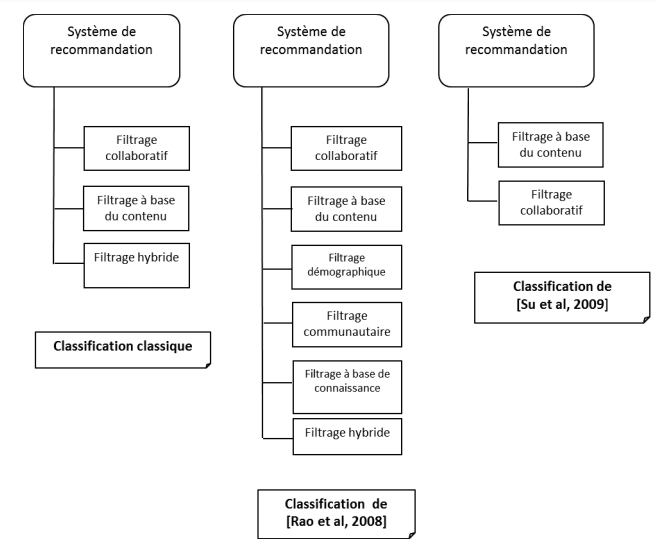
\includegraphics[width=\textwidth]{classification.PNG}
	\caption{classification principale des système de recommandation de \cite{ref5}}
	\label{fig:clas}
\end{figure}


\subsection{Filtrage cognitif }
Dans les systèmes de recommandation basées sur le filtrage cognitif (appelé aussi filtrage basé sur le contenu), le terme « contenu » fait référence aux descriptions des items. 
Les systèmes de recommandation basées sur le contenu font correspondre les utilisateurs à des items similaires à ceux déjà aimés dans le passé.
Selon \cite{ref3}, en général les SR dépendent de deux sources de données:
\begin{itemize}
\item  La première source de données est une description de divers items. Un exemple d'une telle représentation pourrait être la description textuelle d'un article par le fabricant.
\item La deuxième source de données est un profil d'utilisateur, généré à partir des \textit{feedbacks} des utilisateurs sur les divers items, qui peuvent être explicites ou implicites. 
Les feedback explicites peuvent correspondre à des évaluations, tandis que les feedbacks implicites peuvent correspondre à des actions de l'utilisateur tel qu’achat d’article ou historique de recherche.
\end{itemize}

Après l’acquisition de ces deux sources de données, le filtrage cognitif s’effectue selon trois étapes \cite{ref3}:
\begin{enumerate}
	\item  Prétraitement et Extraction de caractéristique des items : les systèmes basés sur le contenu utilisent des descriptifs de type textuel pour les items il faut donc prétraiter ce texte (stemming, suppression de mots vides, extraction de phrase …) et le convertir en une représentation d'espace vectoriel basée sur des mots-clés ou modèle sémantique à base d’ontologies, qui sont une représentation structurée et facilement exploitable par le système. Il s'agit de la première étape de tout système de recommandation basé sur le contenu et elle est hautement spécifique à un domaine (par exemple : un livre a une représentation différente d’une voiture en vue des propriétés que ces 2 objets possèdent).
	\item Apprentissage basé sur le contenu des profils d'utilisateurs : un modèle spécifique est construit pour chaque utilisateur en fonction de leurs antécédents d'achat ou d'évaluation des items, ces 2 derniers sont combinés pour réaliser un profil d'utilisateur qui établit une relation conceptuelle entre les intérêts de l'utilisateur et les attributs des items.
	\item Filtrage et recommandation : dans cette étape, le modèle appris de l'étape précédente (profil utilisateur) et les caractéristiques des items sous forme vectoriel sont utilisés pour formuler des recommandations en calculant une certaine similarité entre les deux, cette similarité permet de définir les items qui sont susceptible d’intéressé l’utilisateur. 
\end{enumerate}

\begin{figure}[H]
	\centering
		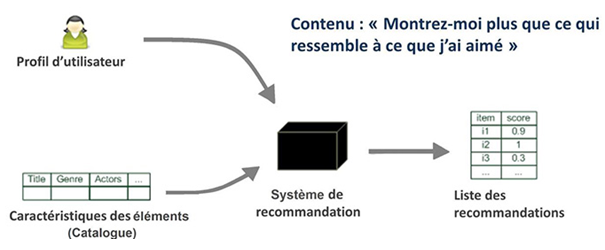
\includegraphics[width=\textwidth]{cognitif.png}
	\caption{SR basé sur le contenu \cite{ref6}}
\end{figure}



 \myparagraph{Avantages et inconvénients du filtrage cognitif}

\begin{itemize}
	\item Avantages 
	\begin{itemize}
		\item Pas besoin d’une communauté d’utilisateurs pour pouvoir effectuer des recommandations aux utilisateurs seul leurs profils suffisent afin de proposer des articles adéquats à leurs besoins. 
		\item Si de nouveaux items sont ajoutés dans la base de données ou s’ils ne sont pas populaires ils peuvent être recommandés 
		\item Transparence : la méthode basée sur le contenu peut nous dire sur quoi elle se base pour suggérer des items.
		\item Pas de démarrage à froid pour les items : contrairement au filtrage collaboratif, de nouveaux éléments peuvent être suggérés avant d'être notés par un nombre important d'utilisateurs.
	\end{itemize}
	\item Inconvénients
		\begin{itemize}
		\item Les systèmes basés sur le contenu ont tendance à rechercher des éléments similaires à ceux que l'utilisateur a vus jusqu'à présent. Ce problème est appelé sur-spécialisation. Il est toujours souhaitable d’avoir une certaine quantité de nouveauté dans les recommandations. \cite{ref3}
		\item Même si les systèmes basés sur le contenu aident à résoudre le problème de démarrage à froid des nouveaux items, ils ne permettent pas de résoudre ce problème pour les nouveaux utilisateurs, lorsqu'il n'y a pas assez d'informations pour créer un profil solide, la recommandation ne peut pas être fournie correctement (Démarrage à froid pour les utilisateurs). \cite{ref7}
		\item Si la description textuelle des items est insuffisante ou inexistante (cas item de type multimédia) la recommandation ne sera pas précise ou ne s’effectuera pas, ce qui peut souvent se produire .\cite{ref7}
		\item Filtrage basé sur la similarité item profil utilisateur donc absence d’autres facteurs comme la qualité de l’item fourni par d’autre utilisateur, le public visé, etc.
		
	\end{itemize}
\end{itemize}

\subsection{Filtrage collaboratif}

Les modèles de filtrage collaboratif utilisent la puissance collaborative des évaluations fournies par plusieurs utilisateurs pour formuler des recommandations, ce type de SR est le plus répondu car il se base sur ce que d’autres utilisateurs ont déjà évalué et apprécié, et cela fait resurgir dans les tendances des articles qui sont bien évalués par la majorité des utilisateurs.

Par exemple, considérons deux utilisateurs A et B, qui ont des goûts très similaires, si les évaluations, que les deux ont spécifiées, sont très similaires, leur similarité peut être identifiée et il est très probable que les évaluations dans lesquelles l’un des deux utilisateurs a spécifié une seule valeur sont également susceptibles d'être similaires. 
Cette similarité peut être utilisée pour déduire des évaluations non spécifiées de A et B pour des items.  

Cette approche peut être appliquée à tout type de documents textuels et multimédias car contrairement au filtrage cognitif, elle ne se base pas sur le contenu des items, mais principalement sur l’exploitation des évaluations que les utilisateurs ont effectué afin de recommander ces mêmes items à d’autres utilisateurs \cite{ref8}.

Il existe deux types de méthodes couramment utilisées dans le filtrage collaboratif, appelées méthodes basées sur la mémoire et méthodes basées sur un modèle \cite{ref3}, le choix de l’approche à utiliser dépendant des informations prises en compte lors du calcul de la prédiction. 

Les deux méthodes partagent les points communs suivants :
\begin{itemize}
\item  Les deux utilisent un calcul de similarité entre les lignes et colonnes d’une matrice appelée « matrice d’usage».
\item Les deux s’effectuent en deux étapes qui sont le calcul de similarité et la prédiction, que nous allons détailler par la suite.
\end{itemize}

\begin{enumerate}[nosep,label=\textbf{\arabic*)}]
	%%\setcounter{enumi}{1}
	\item \textbf{Filtrage collaboratif basé mémoire}
\end{enumerate}\mbox{}\indent Les méthodes basées mémoire sont également appelées algorithmes de filtrage collaboratif basés sur le voisinage. C'étaient parmi les premiers algorithmes de filtrage collaboratif, dans lesquels les évaluations des utilisateur sont prédites sur la base de leurs voisinages\cite{ref3}.

Le voisinage peu être défini de deux manières :
\begin{itemize}
\item Filtrage collaboratif basé sur l’utilisateur : l'idée de base est de déterminer les utilisateurs qui sont similaires à l'utilisateur ciblé A (les voisins de A) en comparant les lignes de la matrice d’usage pour prédire l’évaluation que va donner A, en se basant sur le vote de ses voisins sur le même item. 
Des fonctions de similarité sont calculées entre les lignes de la matrice d’usages pour détecter des utilisateurs similaires.	
\begin{figure}[H]
	\centering
	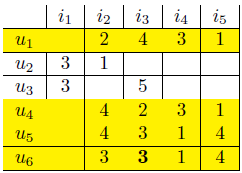
\includegraphics[width=0.25\textwidth]{mat_user_user.png}
	\caption{Matrice d’usage}
\end{figure}
		
	

\item Filtrage collaboratif basé sur les items : le même processus que le FC basé utilisateur est appliqué ici, sauf que dans ce cas la similarité est calculée entre les items et donc entre les colonnes de la matrice d’usage pour détecter les items similaires et les proposer aux utilisateurs qui ont déjà apprécié un item semblable.
\begin{figure}[H]
	\centering
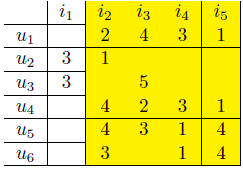
\includegraphics[width=0.25\textwidth]{mat_item_item.png}
	\caption{Matrice d’usage}
\end{figure}


\end{itemize}

\begin{itemize}
	\item Le calcul de similarité:\\
Comme vu précédemment nous avons beaucoup cité les termes « similarité » et « calcul de similarité » afin de déterminer le voisinage des utilisateurs et des items, en effet cette étape est jugés très importante dans les SR basé sur le filtrage collaboratif. Dans cette partie nous allons citer les mesures les plus utilisées dans le FC.

\begin{enumerate}
	\item Calcul similarité utilisateur :\\
	\begin{itemize}
	\item Corrélation de Pearson (COR):\\Pour le calcul de similarité entre deux utilisateurs u et v, la corrélation de Pearson est donnée par la formule suivante :

\begin{equation}\label{key1}
pearson(u,v)=\frac{\sum_{i \in I} (r_{u,i}-\bar{r}_{u}).(r_{v,i}-\bar{r}_{v})}{\sqrt{\sum_{i \in I} (r_{u,i}-\bar{r}_{u})^{2}.(r_{v,i}-\bar{r}_{v})^{2}}}
\end{equation}

où :
\begin{itemize}
	\item r $_{u,i}$ : est l'estimation de l'utilisateur u sur l’item i.
	\item r $_{v,i}$ : est l'estimation de l'utilisateur v sur l’item i.
	\item $\bar{r}_{u}$ : est la moyenne de toutes les notes de l'utilisateur u. 
	\item $\bar{r}_{v}$ : est la moyenne de toutes les notes de l'utilisateur v.
\end{itemize}
\mbox{} 

\item Cosine (COS): \\Le cosinus entre les vecteurs, est une méthode pour calculer le poids de l’utilisateur u$_{i}$  par rapport à l’utilisateur actif u$_{j}$, il est calculé comme un cosinus entre les vecteurs formés par les évaluations des utilisateurs, comme suit :
\begin{equation}\label{key2}
cosine(u_{i},u_{j})=\frac{\sum_{k=1}^{n} r_{u_{i,j}}.r_{u_{i,k}}}{\sqrt{\sum_{k=1}^{n} r_{u_{i,k}}^{2}.\sum_{k=1}^{n}r_{u_{j,k}}^{2}}}
\end{equation}


où :

\begin{itemize}
	\item r$_{u_{i,k}}$  : est l’évaluation de l’utilisateur  u$_{i}$ sur l’item i$_{k}$
	\item r$_{u_{j,k}}$ : est l’évaluation de l’utilisateur  u$_{j}$ sur l’item i$_{k}$
	\item 	n : est le nombre d’item dans le système.
\end{itemize}
\mbox{}\\

\item Calcul similarité items:\\
Le calcul de similarité entre deux items i et j : la corrélation de Pearson est donnée par la formule suivante :

\begin{equation}\label{key3}
pearson(i,j)=\frac{\sum_{u \in U} (r_{u,i}-\bar{r}_{i}).(r_{u,j}-\bar{r}_{j})}{\sqrt{\sum_{u \in U} (r_{u,i}-\bar{r}_{i})^{2}.\sum_{u \in U}(r_{u,i}-\bar{r}_{j})^{2}}}
\end{equation}

où :

\begin{itemize}
	\item r$_{u,i}$  : est l’évaluation de l’utilisateur u sur l’item i 
	\item r$_{u,j}$ : est l’évaluation de l’utilisateur u sur l’item j
	\item $\bar{r}_{i}$ : est la moyenne des évaluations de l’item i par les utilisateurs.
	\item $\bar{r}_{j}$ : : est la moyenne des évaluations de l’item j par les utilisateurs.
\end{itemize}
\end{itemize}

\item Calcul des prédictions:\\
Le calcul de prédiction est une phase importante qui consiste à calculer des prédictions pour générer des recommandations intéressantes à un utilisateur. La plus utilisée pour le calcul de prédictions et la somme pondérée qui considère les plus proches voisins de $u_{i}$ (phase 1) ayant déjà noté l’item i$_{k}$, pour calculer la prédiction de la note de l’utilisateur u$_{i}$ sur i$_{k}$ \cite{ref9}.



\begin{equation}\label{key4}
pred(u_{i},i_{k})=\bar{r(u_{i})} + \frac{\sum_{u_{j} \in U_{i}} sim(u_{i},u_{j}).(r_{u_{j,ik}}-\bar{r(u_{j})})}{\sum_{u_{j} \in U_{i}} sim(u_{i},u_{j})}
\end{equation}

Où: 
\begin{itemize}
	\item sim(u$_{i}$,u$_{j}$) : est la mesure de similarité entre un utilisateur u$_{i}$ et son voisin u$_{j}$, tel que u$_{j}$ $\in$ U$_{i}$.

\end{itemize}


\end{enumerate}
\end{itemize}

\begin{enumerate}[nosep,label=\textbf{\arabic*)}]
	\setcounter{enumi}{1}
	\item \textbf{Filtrage collaboratif basé modèle}
\end{enumerate}\mbox{}\indent Le filtrage collaboratif basé modèle consiste à élaborer des modèles sur lesquels la prédiction va se baser à partir d’une base de données contenant les évaluations faites par les utilisateurs sur les items et une méthode pour la construction du modèle. Il existe plusieurs méthodes pour la construction du modèle, les plus souvent utilisé dans le FC sont le clustering et les réseaux bayésien. 
Le modèle à base de cluster repose sur le principe que certains groupes ou type d’utilisateur capturent un ensemble commun de préférences et de gouts. Étant donné un tel groupe, les préférences concernant les différents items (sous la forme d’évaluations) sont indépendantes. 

Le modèle a base de réseaux bayésien associe un nœud à chaque item. Les états pour chaque nœud correspondent aux valeurs d'évaluations possible pour chaque item. On inclut également un état correspondant à l’absence d’évaluations pour les domaines où il n’y a pas d’interprétation. On peut alors appliquer un algorithme d’apprentissage de réseau bayésien sur la base d’exemple, où les évaluations manquantes sont associées à une valeur « parent » qui sont les meilleures prédictions de ses évaluations\cite{ref10}.

Il existe aussi plusieurs modèle appliqué au filtrage collaboratif pour faire de la recommandation qui sont issues des domaines de recherche sur l’intelligence artificiel comme les réseau de neurone ou les processus décisionnels de Markov, cependant ces techniques font face à certaines problématique car elle sont sensible à l’arrivée de nouveaux utilisateurs ou insertion d’un nouveau item, la phrase d’apprentissage sera ainsi  ré-effectuée au fur et a mesure des mise à jour et connaissant la forte complexité de ces algorithmes elle peut s’avérer très conteuse en temps et en ressource\cite{ref35}. 

\subsubsection*{Avantages et inconvénients du filtrage collaboratif \cite{ref11}:}
\begin{itemize}
	\item Avantages 
	\begin{itemize}
		\item Le filtrage collaboratif se base principalement sur les évaluations des utilisateurs et pas la thématique du contenu à recommander. Ce type de filtrage résout les problèmes liés au filtrage cognitif et donc il permet de filtrer tout type d’information (textuel, multimédia, ressources physiques, image, etc.). L’efficacité du système augmente donc en fonction du nombre d’utilisateurs.
		\item Absence de l’effet entonnoir, car si un item est évalué, il peut alors être recommandé ce qui permet à l’utilisateur de découvrir divers domaines intéressants auxquels il n’avait pas pensé. 
		\item Possibilité de prendre en considération d’autres facteurs et critères des items tels que la qualité de l’information, le public visé, etc. 
	\end{itemize}
	\item Inconvénients
	\begin{itemize}
		\item Démarrage à froid : toute nouvelle ressource ne peut être recommandée car elle n’a pas encore été évaluée. De même, pour un nouvel utilisateur, le système ne peut pas lui recommander une ressource car tant qu’il n’a pas effectué d’évaluations il ne pourra pas faire partie d’une communauté d’utilisateurs.
		\item Pour former de meilleures communautés, le système exige un nombre suffisant d’évaluations en commun entre les utilisateurs pour pouvoir les rapprocher (i.e. décider s’ils appartiennent au même voisinage).		
	\end{itemize}
\end{itemize}

\subsection{Filtrage hybride}
Le filtrage hybride combine les deux algorithmes précédent (et/ou d'autres algorithmes), selon les méthodes suivantes:\cite{ref12}:
\begin{itemize}
	\item Pondérée : Les résultats pondérés de plusieurs techniques de recommandation sont combinés pour produire une nouvelle recommandation.
	\item Permutation : Le système permute entre les différentes techniques de recommandation selon le résultat de la recommandation.
	\item Mixte : Les recommandations de plusieurs techniques sont présentées en même temps
	\item  Combinaison : Différentes techniques de recommandation sont combinées en un unique algorithme de recommandation
	\item  En cascade : Un système de recommandation raffine les résultats fournis par un autre système.
	\item Augmentation : Le résultat "output" d'une technique de recommandation est utilisé comme données en entrée "input" pour l'autre technique.
	\item Méta-niveau : Le modèle appris par une technique de recommandation est utilisé comme données en entrée pour l'autre technique.
\end{itemize}
\section{Autre Système de recommandation}
Étant donné que les filtrages présentés précédemment ne prennent pas en compte l’aspect sémantique existant dans la description des items ou dans les besoins récoltés des évaluations des utilisateurs, nous expliquons dans ce qui suit le fonctionnement du filtrage sémantique et les mesures similarité qu'il utilise.
\subsection{Filtrage sémantique}
Afin de surpasser les limitations du filtrage collaboratif et obtenir de meilleurs résultats, nous proposons une amélioration en combinant ce dernier avec le filtrage sémantique. La notion de sémantique qui est représentée par les ontologie va nous permettre d’établir une relation entre les utilisateurs et les items, et relier ces derniers entre eux. Ces relations permettent d'avoir un filtrage plus précis.

\myparagraph{Définitions d’ontologie}	
D’après \cite{ref13}, une ontologie est une spécification explicite d'une conceptualisation. 
Plus concrètement, une ontologie est une description explicite des concepts et les relations entre ces derniers.Dans une ontologie, les concepts sont représentés par une classe décrite par un titre et un ensemble d'attributs. Une classe peut être une sous-classe d'une autre. L'ensemble des classes et les relations entre eux constitue une ontologie.
\begin{figure}[H]
	\centering
	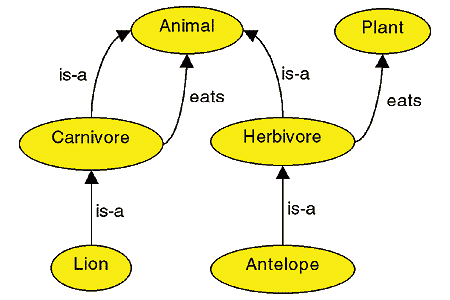
\includegraphics[width=0.7\textwidth]{ontologie_Exemple.png}
	\caption{Une ontologie du concept animal \cite{ref29} }
\end{figure}
	
	
\myparagraph{Systèmes de recommandation avec modèles sémantiques à base d’ontologie}
Dans le domaine du web sémantique, les recherches qui tentent d'améliorer les systèmes de recommandations ont connu une croissance, cette approche construit une hiérarchie des catégories (arborescence des concepts) dont les items sont les feuilles. Elle construit des informations sémantiques sur ces derniers et les profils des utilisateurs afin de représenter les relations entre eux, et entre les items et les utilisateurs.

\myparagraph{Méthodes de mesures de similarités sémantiques}
Il y a plusieurs méthodes du calcul de similarité sémantique,  peuvent être diviser en quatre catégories majeurs d’après \cite{ref14}:
	\begin{enumerate}
		\item Comptage des arcs entre deux concepts \textit{(Edge Counting}).
		\item Approche basée sur le contenu informationnel \textit{(Information Content}).
		\item Méthodes basées sur les fonctionnalités. (\textit{Feature-Based})
		\item Méthodes hybrides.
	\end{enumerate}
Dans notre travail nous nous intéressons à la méthode de comptage d'arc, de ce fait nous allons la décrire dans ce qui suit.
\myparagraph {Le comptage des arcs entre deux concepts}
C’est une méthode qui utilise les ontologies sous forme d’arborescence. Elle consiste à calculer la distance entre deux concepts (le nombre des arcs qui séparent ces derniers). Ce calcul dépend très fortement de la profondeur dans laquelle se trouvent les deux concepts en question, car la similarité entre les concepts spécifiques est bien plus grande que celle des concepts généraux (plus deux concepts sémantiquement proches sont profonds dans l'arborescence plus leur similarité augmente). Il existe plusieurs techniques de comptage d'arcs, parmi ces techniques: 
	\begin{itemize} 
	\item Rada : Les mesures de similarité sémantique basées sur les arcs ont été introduites par \cite{ref15}. Elles ont été définies en fonction de la distance qui sépare deux concepts. La mesure est donnée par la formule suivante:
	\begin{equation}
	Sim_{con}= \frac{1}{1 + dist(c1, c2)}  = \frac{1}{1 + N1 + N2} 
	\end{equation}
		\begin{figure}[H]
		\centering
		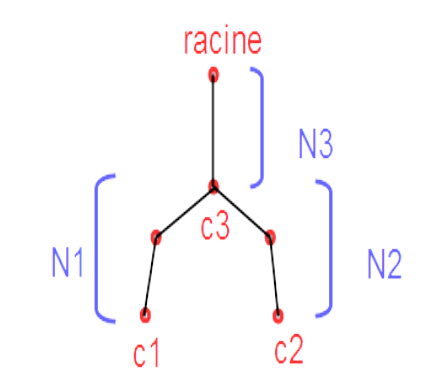
\includegraphics[width=0.5\textwidth]{rada.PNG}
		\caption{Exemple de taxonomie pour les mesures de similarité basées sur les arcs}
		\label{fig:rada}
	\end{figure}

	\item Wu et Palmer : Soit C1 et C2 deux concepts dont nous allons calculer la similarité. Le principe de calcul de similarité est basé sur la distance (N1 et N2) séparant C1 et C2 du nœud racine et la distance (N) séparant l'ancêtre commun le plus proche (CS) de C1 et C2 du nœud R (voir figure ~\ref{fig:wupalm}). La mesure de similarité de \cite{ref37} est définie par la formule suivante:
	\begin{equation}\label{key6}
	Dist_{WP}= \frac{ (2*N)}{(N_{1}+N_{2}+2*N)}  
	\end{equation}
		\begin{figure}[H]
			\centering
			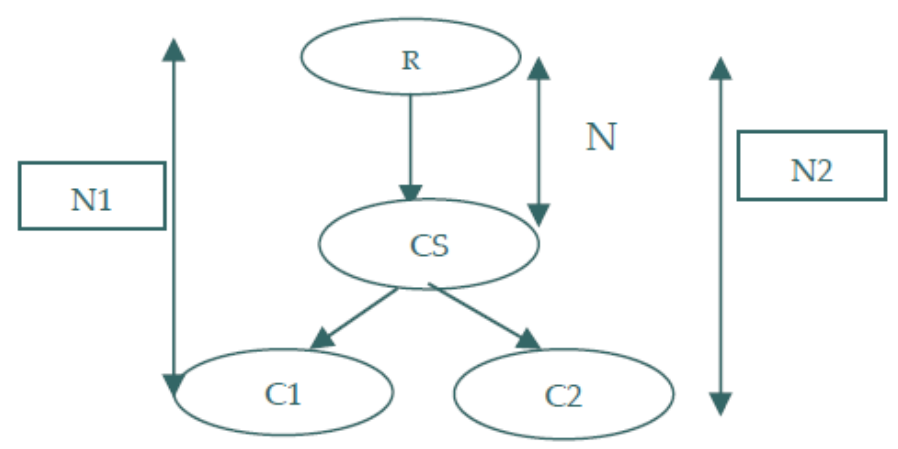
\includegraphics[width=0.8\textwidth]{wupal.PNG}
			\caption{Exemple de hiérarchie de concepts \cite{ref38}}
			\label{fig:wupalm}
		\end{figure}
	
		
	\end{itemize}

\section{Construction du profil utilisateur}
L’utilisateur est au centre des systèmes de recommandation, il est à la fois consommateur et contributeur. Ainsi, la bonne qualité des informations sur les utilisateurs est une condition nécessaire pour l’efficacité des systèmes de recommandation. Ces informations sont stockées dans le profil utilisateur, qui se définit généralement comme une structure permettant de stocker et modéliser les préférences des utilisateurs et leurs centres d’intérêts\cite{ref20}.

\subsection {Caractéristiques du profil utilisateur }
Le profil utilisateur peut être décomposé en deux catégories \cite{ref21}:
\begin{enumerate}
	\item Caractéristiques explicites
	Les caractéristiques explicites sont généralement objectives, elles se basent sur les informations fournies par l’utilisateur directement, indiquant ses centres d’intérêts, ses connaissances, ses préférences, ses objectifs, etc. Exemple: demander à un utilisateur de commenter, taguer, aimer (\textit{liker}), ajouter comme favoris des contenus qui l’intéressent. 
	On utilise souvent une échelle d’évaluations allant d'une étoile (je n’aime pas du tout) à cinq étoiles (j’aime beaucoup), qui sont ensuite transformées en valeurs numériques afin de pouvoir être utilisées par les algorithmes de recommandation \cite{ref22}.
	\item 	Caractéristiques implicites :
	Les caractéristiques implicites sont généralement subjectives et difficiles à capter. Mais, contrairement aux caractéristiques explicites, elles contiennent plus d’information sur les besoins de l’utilisateur. Ces caractéristiques sont détectées à travers des comportements observables recueillis par le système lorsque l’utilisateur interagit avec son environnement \cite{ref23}.
	\item Elles sont inférées à partir de:
	\begin{itemize}
		\item Activités de navigation.
		\item Évaluations, annotations (étiquetages, tags).
		\item Analyse du réseau social de l’utilisateur.
		\item Liste des éléments que l’utilisateur à écoutés, regardés ou achetés en ligne.
		\item Documents et pages web consultés et le temps passé sur chaque page, etc.
		\item Clique de la souris sur une page (document).
		\item Enregistrement/impression d’un document.
		\end{itemize}
\end{enumerate}
L’avantage d’utiliser des techniques implicites pour la construction du profil de l’utilisateur est que ce dernier est allégé de certaines actions (définition de ses préférences, se son caractère, etc.) \cite{ref11}.
\subsection{Modèle de représentation du profil de l’utilisateur}
Modéliser l’utilisateur, ses centres d’intérêts, ses préférences et son besoin d’information est une tâche très importante dans les systèmes de recommandation. Pour cela, il faut tout d’abord définir la structure du profil qui nous permettra de stocker toutes les informations qui le concernent. Dans cette section, nous allons décrire les modèles les plus répandus dans la littérature pour représenter et structurer les profils des utilisateurs.

\begin{enumerate}
	\item Modèle vectoriel :\\
	C’est le modèle basique d’espace vectoriel de \cite{ref24}. Dans cette représentation, le contenu du profil utilisateur est caractérisé par un ou plusieurs vecteurs de termes pondérés. Ces termes sont obtenus à partir de plusieurs sources d’information recueillies sur l’utilisateur.\\
	Selon \cite{ref25} la plupart des systèmes de recommandation utilisent le modèle d’espace vectoriel (MEV), qui est une représentation spatiale des documents textuels où chaque document est caractérisé par un vecteur de poids sur des termes appartenant à l’ensemble des termes d’une collection de documents. La pondération des termes est généralement basée sur le format TF-IDF (\textit{term frequency-inverse document frequency}). Le poids associé à chaque terme représente son degré d’importance dans le profil utilisateur. 
	
	\begin{itemize}
		\item 	D= (d$_{1}$, d$_{2}$, …, d$_{N}$) : collection de documents.
		\item 	T= (t$_{1}$, t$_{2}$, …, t$_{N}$) : l’ensemble de tous les termes appartenant à la collection de document D. 
	\end{itemize}
	Chaque document $d_{j}$ figurant dans les préférences de l’utilisateur sera donc représenté dans son profil par un vecteur de dimension n tel que, dj= \{ w$_{1j}$, w$_{2j}$, …, w$_{nj}$ \}, ou w$_{kj}$ est le poids associé au terme t$_{k}$ dans le document.
			
	
	
 \subsubsection{ Avantages et inconvénients de ce modèle  \cite{ref27}}
\begin{itemize}
	\item  Avantages : Le modèle vectoriel à l’originalité d’être simple à mettre en œuvre, et la prise en compte de plusieurs centres d’intérêts de l’utilisateur en utilisant plusieurs vecteurs.  
	\item  Inconvenients : pas d’ordonnancement entres les préférences et les centres d’intérêts des utilisateurs, et pas de considération de l’aspect sémantique (i.e. pas de liens entres les termes).
\end{itemize}


 \item Modèle sémantique à base d’ontologies : Les ontologies sont utilisées pour représenter les relations sémantiques entre les unités d’informations constituant le profil utilisateur. Dans ce modèle, le profil utilisateur est vu comme une hiérarchie de concepts pondérés \cite{ref26}, où chaque nœud dans la hiérarchie est un concept associé à un poids représentant l’intérêt porté par l’utilisateur sur ce concept.  Le contenu de chaque concept peut être souvent représenté par un vecteur défini dans un espace de termes pondérés. La représentation du profil utilisateur avec le modèle sémantique à base d’ontologie aide à mieux connaître les intérêts des utilisateurs par rapport au modèle vectoriel. De plus la valeur d’intérêt d’un concept peut être propagée vers les autres concepts sémantiquement liés, dans le but de trouver de nouveaux centres d’intérêts.

 
 \begin{figure}[H]
 	\centering
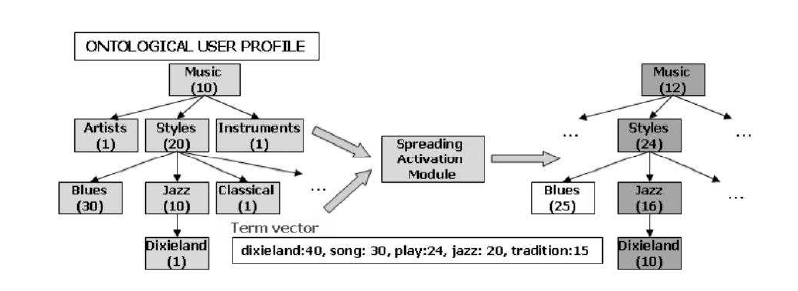
\includegraphics[width=\textwidth]{profile_user.PNG}
 	\caption{ Exemple de profil utilisateur représenté par le modèle d’ontologies avec le processus de mise à jour des poids des concepts \cite{ref28}}
 \end{figure}
 

\end{enumerate}

\section {Travaux liés}
Dans cette partie nous nous intéressant aux travaux existants (Sémantique, hybridation entre sémantique et collaboratif), afin de proposer par la suite une contribution et la comparé à ces travaux. Nous allons citer deux travaux liés et qui sont:

\subsection{Recommandation hybride par Filtrage sémantique et FC multicritères}

\begin{itemize}	
\item Le travail présenté par Shambour et Lu \cite {ref36} propose une hybridation du filtrage sémantique avec le FC multicritères.


\item 	Problématique :  Le Filtrage collaboratif (CF) est probablement la technique la plus populaire dans les systèmes de recommandation. Malgré son succès dans diverses applications, les techniques basées sur les FC rencontre une limitation majeure, qui est le démarrage à froid. Par conséquent les chercheurs ont proposé une approche hybride multi-critères sémantiquement renforcée du filtrage FC (MC-SeCF) afin de palier à cette problématique.\cite {ref36}. 

\item 	Résultat obtenu : Les résultats expérimentaux vérifient l’efficacité de l’approche hybride pour atténuer le problème de faible densité de données et de démarrage à froid en obtenant une meilleure précision et une plus grande couverture dans les cas du démarrage à froid et l’arrivé de nouvelles données, que les algorithmes de recommandation FC basés sur les items \cite {ref36}. 
\end{itemize}

\subsection{Un système de recommandation basé sur une clustering multivues de similarité et de confiance}
\begin{itemize}	
\item Le travail présenté par Gu et al. \cite{ref30} propose un clustering Multivues, une vue similarité et une vue basée sur la confiance.

\item 	Problématique : Bien que le clustering a démontré qu’il est efficace et évolutif pour des ensembles de données à grande échelle, les système de recommandation qui se base sur le clustering souffrent d'une précision et d'une couverture relativement faibles. Pour résoudre ces problèmes, les chercheurs ont développé une méthode de clustering multivues  par laquelle les utilisateurs sont mis dans les clusters de manière itérative à partir des deux vues de similarité et de confiance ente les utilisateurs\cite{ref30}.

\item	Résultat obtenu : Les résultats expérimentaux ont été effectuer sur trois ensembles de données du monde réel, et démontrent que leurs approche peut effectivement améliorer à la fois l'exactitude et la couverture des recommandations\cite{ref30}.
\end{itemize}
	
\section {Conclusion}
Dans ce chapitre nous avons présenté la recommandation, son utilité et les notions liées à cette dernière, suivie des techniques de recommandation les plus utilisés : le filtrage cognitif, collaboratif et hybride, nous avons vu leurs fonctionnements, avantages et inconvénients. 
La représentation des profils d’utilisateur est une étape importante dans les SR, et elle est souvent effectuée à l’aide de deux modèles:  modèle vectoriel et le modèle basé sur les ontologies.
Les techniques de filtrage vu précédemment sont très répondu et utilisé, et peuvent t’être améliorées et optimisées en utilisant d’autres technique issue de l’intelligence artificielle comme le clustering et métaheurstique, que nous allons présenter dans le prochain chapitre. 


\newpage
\chapter{Classification et optimisation}
\thispagestyle{empty}
\newpage
\section{Introduction}
Depuis la naissance de l’internet et les réseaux sociaux, le volume des données digitales a connu une croissance rapide et exponentielle. Ces données sont principalement sous forme brute, et sans aucune structure définie avec des volumes de Teras Octets, d'où la nécessité des nouvelles méthodes optimisées pour la classification de ces données et extraire les informations pertinentes. Avec l’IA (Intelligence Artificielle), le monde de la recherche travaille pour introduire et développer de plus en plus ces méthodes pour atteindre de meilleurs résultats.

Dans ce chapitre, nous allons introduire quelques méthodes de classifications et optimisations dont on s'est intéressé pour effectuer notre travail.       

La structuration du chapitre est la suivante:
\begin{itemize}
	\item Classification supervisé et non supervisée,
	\item Optimisation avec métaheurstiques,
	\item Optimisation dans les système de recommandation,
	\item Conclusion.
\end{itemize}

\section {classification}
La classification est une répartition des êtres vivants, des objets, ou des notions sur plusieurs classes. C’est un processus utilisé dans la science en particulier afin d'effectuer des études et des analyses.
En biologie par exemple, la classification est utilisée pour catégoriser les animaux, les végétaux, et plusieurs micro-organismes.

La classification en informatique est un processus qui prend un ensemble de données brutes, et essaye de créer un modèle de classification, qui les répartis d’une façon correcte. Il existe plusieurs types de modèles de classification et qui sont divisés en deux catégories :

\subsection{ Modèles supervisés}
Un modèle de classification supervisé est construit en deux étapes:
	\begin{enumerate}

		\item L’apprentissage: dans cette étape on introduit en entrée au modèle un ensemble de données dont les classes sont connues au préalable, et à chaque  fois qu'on lui envoie une nouvelle instance pour qu'il effectue une prédiction de sa classe, on mesure la performance du modèle afin de l'ajuster, on répète ce processus jusqu'à ce qu'il commence à reconnaître les classes des données correctement.
		
		\item Le test: après la fin de l’étape d’apprentissage, on introduit au modèle un ensemble de données qu’il n’a jamais traité auparavant, une prédiction des classes des données est effectuée ensuite une mesure des performances. Quand le modèle reconnaît parfaitement les données qu’on lui donne ou s'il possède un taux d’erreur qui est considéré comme négligeable, on peut dire que le modèle est près pour l’utilisation commerciale.	
	\end{enumerate}


Dans un tel modèle, les classes et leurs nombres sont connus préalablement, donc le modèle ne va jamais reconnaître une instance ayant une nouvelle classe.

Nous nous intéressons dans notre travail au modèle \textit{K-NN}, de ce fait nous allons le définir et expliquer son fonctionnement.

\myparagraph{K-NN:}La méthode des K plus proches voisins est une méthode d’apprentissage supervisé. En abrégé K-NN, de l'anglais \textit{k-nearest neighbors}, inventé par Marcello Pelillo en 1967. Elle peut être utilisée aussi bien pour la régression que pour la classification. Son fonctionnement peut être assimilé à l’analogie suivante “dis moi qui sont tes voisins, je te dirais qui tu es”.
Pour effectuer une prédiction, l’algorithme K-NN va se baser sur le jeu de données en entier, ceci peut être considéré comme l'ensemble d'entraînement pour l'algorithme, bien qu'un entraînement explicite ne soit pas particulièrement requis. En effet, pour une observation, qui ne fait pas parti du jeu de données, qu’on souhaite prédire, l’algorithme va chercher les K instances du jeu de données les plus proches de notre observation. Ensuite pour ces K voisins, l’algorithme se basera sur leurs variables de sortie (\textit{output variable}) pour calculer la valeur de la variable de l’observation qu’on souhaite prédire. 

Par ailleurs  :
\begin{itemize}
	\item Si K-NN est utilisé pour la régression, c’est la moyenne (ou la médiane) des variables des K plus proches observations qui servira pour la prédiction
	 \item Si K-NN est utilisé pour la classification, c’est le mode des variables des K plus proches observations qui servira pour la prédiction\cite{ref32}.
\end{itemize}

 \begin{algorithm}[H]
	\caption{K-NN}
	\hspace*{\algorithmicindent} \textbf{Entrée:} D: Dataset, K: nombre de voisins à considérer ;\\
	\hspace*{\algorithmicindent} \textbf{Sortie:} K clusters ; \\
	\hspace*{\algorithmicindent}\textbf{ Début:}
	\begin{itemize}
		\item [] \textbf{Pour} une nouvelle observation X dont on veut prédire sa variable de sortie y \textbf{faire:}
		\begin{itemize}
			\item [] Calculer toutes les distances de cette observation X avec les autres observations du jeu de données D ;
			\item [] Retenir les K observations du jeu de données D les proches de X en utilisation le fonction de calcul de distance d ;
			\item [] Prendre les valeurs de y des K observations retenues: \begin{itemize}
				\item [] Si on effectue une régression, calculer la moyenne (ou la médiane) de y retenues ;
				\item [] Si on effectue une classification , calculer le mode de y retenues ; 	
			\end{itemize}
			\item [] Retourner la valeur calculée dans l’étape 3 comme étant la valeur qui a été prédite par K-NN pour l’observation X ;
		\end{itemize}

	\end{itemize}
	\hspace*{\algorithmicindent}\textbf{ Fin.}
\end{algorithm} 

\subsection{ Modèles non supervisés \textit{(Clustering)}}
Contrairement aux modèles supervisés, ils n'effectuent pas d’apprentissage, car ils sont censés deviner les classes des objets en trouvant les similarités et les différences entre les instances des données. On appelle la similarité/différence entre deux instances, la distance entre eux. Un ensemble d'éléments groupés sont appelés un cluster. La notion de cluster varie d’une application à une autre selon les besoins et les nécessités. Elle est généralement reliée au type de dataset, et les mesures de la distance entre les instances. Dans un tel modèle on n'est pas limité par le nombre de classes car on ne connaît pas les classes au préalable.

Il y a plusieurs algorithmes qui font partie du domaine de la fouille de données (\textit{Data Mining}) qui s’adresse au problème de la classification non supervisée (\textit{clustering}). Les techniques et algorithmes de clustering sont très utilisés dans plusieurs domaines pour l’analyse des données.

\subsubsection*{Les différents types de méthodes de cluestring}
D’après Han et al.\cite{ref33}, les algorithmes de clustering sont divisés comme suit :\\

\begin{enumerate}[nosep,label=\textbf{\arabic*)}]
	%%\setcounter{enumi}{1}
	\item \textbf{Méthodes de partitionnements}
\end{enumerate}\mbox{}\indent C’est l’approche la plus simple, étant donnée un nombre \textit{N}, elle consiste à partitionner le dataset en \textit{N} groupes ou clusters initialement. Après, une technique de re-locations est utilisée de façon itérative pour améliorer le partitionnement en déplaçant les instances d’un groupe à un autre. Le critère général pour un bon partitionnement est que les instances d’un même cluster soient proches, et les instances des différents clusters soient loin. Parmi les les algorithmes les plus connus: KNN, K-means, K-medoïds, CLARANS, ...etc.  \\



\begin{enumerate}[nosep,label=\textbf{\arabic*)}]
	\setcounter{enumi}{1}
	\item \textbf{Méthodes hiérarchiques}
\end{enumerate}\mbox{}\indent Elles consistent à créer une décomposition hiérarchique de l'ensemble de données et est classée comme étant soit agglomération ou division, en fonction de la formation de la décomposition hiérarchique. L’approche agglomérative, également appelée approche ascendante, commence par mettre chaque instance dans un groupe séparé puis des fusions successive sont effectuées sur les instances ou les groupes d'instances proches les uns aux autres jusqu'à ce que tous les groupes soient fusionnés en un seul (le niveau le plus élevé de la hiérarchie) ou une condition de terminaison est remplie. L’approche de division, également appelée la approche descendante, commence par mettre les instances dans un même cluster, puis à chaque itération, un cluster est divisé en clusters plus petits, jusqu'à ce que chaque instance soit finalement dans un cluster, ou une condition de terminaison est valide. 
Les méthodes de classification hiérarchique peuvent être basées sur la distance ou sur la densité et la continuité. Les méthodes hiérarchiques souffrent du fait qu’une fois l’étape est terminée (fusion ou division), elle ne peut jamais être défaite. Cette rigidité est utile car elle conduit à des calculs plus petits. Parmi les algorithmes les plus connus: AGNES, et DIANA.\\

\begin{enumerate}[nosep,label=\textbf{\arabic*)}]
	\setcounter{enumi}{2}
	\item \textbf{Méthodes basés sur la densité}
\end{enumerate}\mbox{}\indent C’est une amélioration de la méthode de partitionnement. Dans les méthodes basées sur la  densité, un cluster continue à grandir à condition que le nombre d’instances dans un rayon de voisinage est supérieur à un seuil donné. Une telle méthode peut filtrer le bruit et les valeurs aberrantes. Parmi les algorithmes on mentionne \textit{DBSCAN}, et \textit{DENCLUE}.\\


\subsubsection*{Quelque Algorithmes de clustering }

\begin{enumerate}[nosep,label=\textbf{\arabic*)}]
	%%\setcounter{enumi}{1}
	\item \textbf{K-means}
\end{enumerate}\mbox{}\indent Étant donné un dataset et un nombre K de clusters, l’algorithme commence par choisir K instances aléatoires qui représentent les centroids initiaux et affecte le reste des instances aux clusters ayant le plus proche centroid. Après, il calcule les nouveaux centroids pour chaque cluster, et refait le processus jusqu'à ce qu'il n'y est plus de changement.
Cet algorithme est très sensible aux données aberrantes, par conséquent il ne garantit pas l’optimum global, mais il a l'avantage de converger vers un optimum local quelles que soient les données initiales.
Le calcul des centroids se fait en général par la moyenne. Étant donné un cluster, le centroid est une instance dont la valeur de chaque attribut est la moyenne des valeurs du même attribut des instances appartenant à ce cluster \cite{ref33}.
 \begin{algorithm}[H]
	\caption{k-means}
	\hspace*{\algorithmicindent} \textbf{Entrée:} D: Dataset, K: nombre de cluster ;\\
	\hspace*{\algorithmicindent} \textbf{Sortie:} K clusters ; \\
	\hspace*{\algorithmicindent}\textbf{ Début:}
	\begin{itemize}
		\item [] Choisir les centreoids initials à partir de D aléatoirement ;
		
		\item []\textbf{Répéter:}
		\begin{itemize}
			\item []\textbf{Pour} Chaque p de D \textbf{faire:} 
			\begin{itemize}
				\item [] Calculer la similarité entre p et les centroids  ;
				\item [] Affecter p au cluster qui possède le plus proche centroids ;
			\end{itemize}
			\item []\textbf{Fait;}
			\item [] Calculer les nouveaux centroids (la moyenne);
		\end{itemize}
	\end{itemize}
	\hspace*{\algorithmicindent}\textbf{ Fin.}
\end{algorithm} 
\mbox{}\\

\begin{enumerate}[nosep,label=\textbf{\arabic*)}]
	\setcounter{enumi}{1}
	\item \textbf{K-medoids}
\end{enumerate}\mbox{}\indent C’est une amélioration  de K-means qui le rend plus efficace pour traiter les données aberrantes. K-medoid utilise comme centroids, des instances du dataset  appelé medoids. La base de cette approche est de trouver les K instances du dataset qui peuvent représenter les centres des clusters à former. 

Une variation populaire de cette approche est \textit{PAM}(\textit{Partitioning Around Medoids}), cet algorithme commence par un choix aléatoire des medoïds à partir du dataset initial, et affecte les instances du dataset au cluster possédant le plus proche medoid, par la suite chaque medoid est remplacé soit d'une façon aléatoire ou avec heuristique, s'en suit un calcul du coût de remplacement, si le clustering est amélioré alors la permutation des medoids est gardée, et le processus est répété jusqu'à ce que aucun changement est effectué \cite{ref33}.


 \begin{algorithm}[H]
	\caption{k-medoids}
	\hspace*{\algorithmicindent} \textbf{Entrée:} D: Dataset, K: nombre de cluster ;\\
	\hspace*{\algorithmicindent} \textbf{Sortie:} K clusters ; \\
	\hspace*{\algorithmicindent}\textbf{ Début:}
	\begin{itemize}
			\item [] initialiser les K medoids aléatoirement ;
		
		\item []\textbf{Répéter:}
		\begin{itemize}
			\item [] Affecter les instances de D au cluster qui convient ;
			\item []\textbf{Pour} Chaque p de D \textbf{faire:} 
			\begin{itemize}
			\item [] Calcul du coût S de swap d’un medoïd mj avec p ;
			 \item []\textbf{Si:} S < 0 \textbf{Alors} swap mj avec p \textbf{Fsi} ;
			\end{itemize}
			\item []\textbf{Fait;}
		\end{itemize}
		\item []\textbf{Jusqu'à: }aucune changement ;
		
	\end{itemize}
	\hspace*{\algorithmicindent}\textbf{ Fin.}
\end{algorithm} 


\section{Optimisation avec \textit{métaheuristiques}}

Dans le but d’améliorer les performances du système  à implémenter et la qualité des résultats, on a choisi d'appliquer une technique d’optimisation appelée métaheuristiques.     

Les métaheuristiques sont utilisées pour trouver des réponses à des problèmes dont on n'a que très peu d'éléments pour le résoudre, c'est a dire que nous ne savons pas à quoi ressemble la solution optimale, ni comment la trouver de manière raisonnée, il y a très peu de renseignements heuristiques et la recherche par force brute est impensable, car l'espace de recherche est trop grand. 
Néanmoins, si une solution candidate au problème nous est fournie, nous sommes capables de la tester et d'évaluer sa qualité et de répéter le processus jusqu'à avoir la solution adéquate (taux d'erreur moindre).

Un des algorithmes de métaheuristiques les plus simples, est la méthode de descente \textit{Hill-Climbing}: à partir d’un ensemble de valeurs prises aléatoirement, une petite modification aléatoire est effectuée. Si la modification améliore l’ensemble, on la garde, sinon elle est rejetée. Ce processus est effectué autant qu’il est possible. De nombreuses métaheuristiques sont essentiellement élaborées par des combinaisons de cette méthode et de la recherche aléatoire.

\subsection{Bee Swarm Optimisation (BSO)}

L'algorithme BSO (Bee Swarm Optimisation) est l'algorithme d'optimisation par essaim d'abeilles. BSO se base sur la simulation d’un ensemble d'abeilles qui cherche la nourriture. On suppose que l’espace de recherche est représenté par l’ensemble de solutions possibles, et la richesse de la nourriture par la qualité de la solution. Le processus naturel se déroule comme suit :
\begin{itemize}
\item L'abeille éclaireuse qui découvre une quantité de nectar et retourne à la ruche.
\item Elle effectue ensuite une danse circulaire, pour signaler qu’elle a trouvé une source de nourriture.
\item La danse qu’elle effectue dépend de la qualité de la source, et la distance entre la ruche et la source, ainsi que la direction \cite{ref34}.
\end{itemize}

Selon \cite{ref34}, voici le déroulement de l’algorithme BSO :
\begin{enumerate}

\item	On génère une solution aléatoire appelée \textit{Sref}(solution de référence).
\item	On met \textit{Sref} dans une liste taboue.
\item	À partir de \textit{Sref}, un ensemble de points est déterminé.
\item	Chaque point généré est attribué à une abeille (recrutement).
\item	Chacune des abeilles effectue une recherche locale commençant par le point qu’est lui y est attribué.
\item	Les abeilles placent leurs meilleurs résultats dans un tableau pour les comparer.
\item	La meilleure solution dans le tableau est choisie comme le nouveau point \textit{Sref}, et on réitère le processus depuis (2). 
\end{enumerate}
\begin{figure}[H]
	\centering
	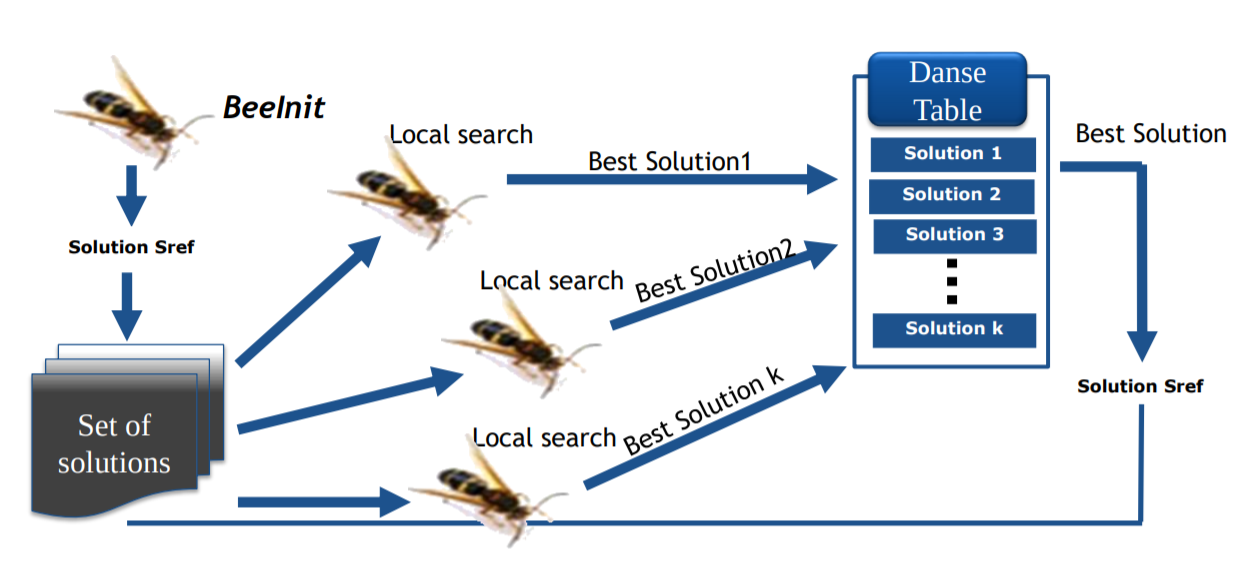
\includegraphics[width=\textwidth]{bso.PNG}
	\caption{ Schéma expliquant le fonctionnement de BSO \cite{ref34} }
\end{figure}
\subsection{Optimisation dans les systèmes de recommandations}
Il existe plusieurs approches pour l'incorporation des méthodes d’optimisation dans un système de recommandation, afin d’améliorer les résultats.
L’une des approches est d’utiliser les caractéristiques des utilisateurs pour un filtrage collaboratif, et donner des priorités à ses caractéristiques en ajoutant des poids. Dans ce cas une métaheuristique peut être utilisée pour trouver les poids qui donnent un résultat optimal. Cette approche a été réaliser par \cite{ref31} qui ont utilisé l’algorithme PSO pour l’optimisation. Dans notre travail, on utilise les algorithmes de clustering pour la recommandation et afin d'obtenir les résultats les plus optimaux, on utilise aussi une métaheuristique pour affiner leurs paramètres et ainsi améliorer la qualité des prédictions.
\section {Conclusion}
Dans ce chapitre nous avons présenté quelques méthodes de classification et optimisation, et expliqué leurs fonctionnement, dans le prochain chapitre nous allons implémenter ces méthodes avec quelques types de filtrages choisi afin d'améliorer la qualité de prédiction effectuer par ces derniers.
\chapter{Conception}
\thispagestyle{empty}
\newpage
\section{Introduction}
Ayant pour objectif d’augmenter les performances du filtrage collaboratif, sémantique et leurs hybridation nous proposons une approche qui utilise le clustering optimisé afin d'améliorer le partitionnement des utilisateurs (ou des items) en vue d’effectuer des recommandations plus précises. Ce chapitre sera structuré de la façon suivante:
\begin{itemize}
	\item Description de l'approche de recommandation par classification,
	\item Les différents types de filtrage conçu et leurs fonctionnement,
	\item L'aspect de classification ajoutée aux filtrages réalisés;
	\item L'optimisation de la classification avec une métaheurstique (BSO),
	\item Conclusion.
\end{itemize}

\section{Description de l'approche de recommandation par classification}
Les étapes de notre approche peuvent être résumées comme suit:
\begin{itemize}
\item Conception du filtrage collaboratif (FC),
\item Conception du filtrage sémantique (FSem),
\item Réalisation de trois différentes hybridations basées sur les deux filtrage FC et FSem,
\item Améliorer les algorithmes de filtrage conçu en leurs appliquant des techniques de classification,
\item Réalisation d'une hybridation multiview (hybridation selon deux ou plusieurs aspects, dans notre cas l'aspect collaboratif et sémantique),
\item  Optimisation des différents filtrage conçu avec une méta-heuristique.
\end{itemize}
La figure  ~\ref{fig:shema} illustre les différents algorithmes de notre approche de recommandation, par la suite nous allons présenter en détail chacun de ces algorithmes dans les sections qui suivent.
\begin{figure}[H]
	\centering
	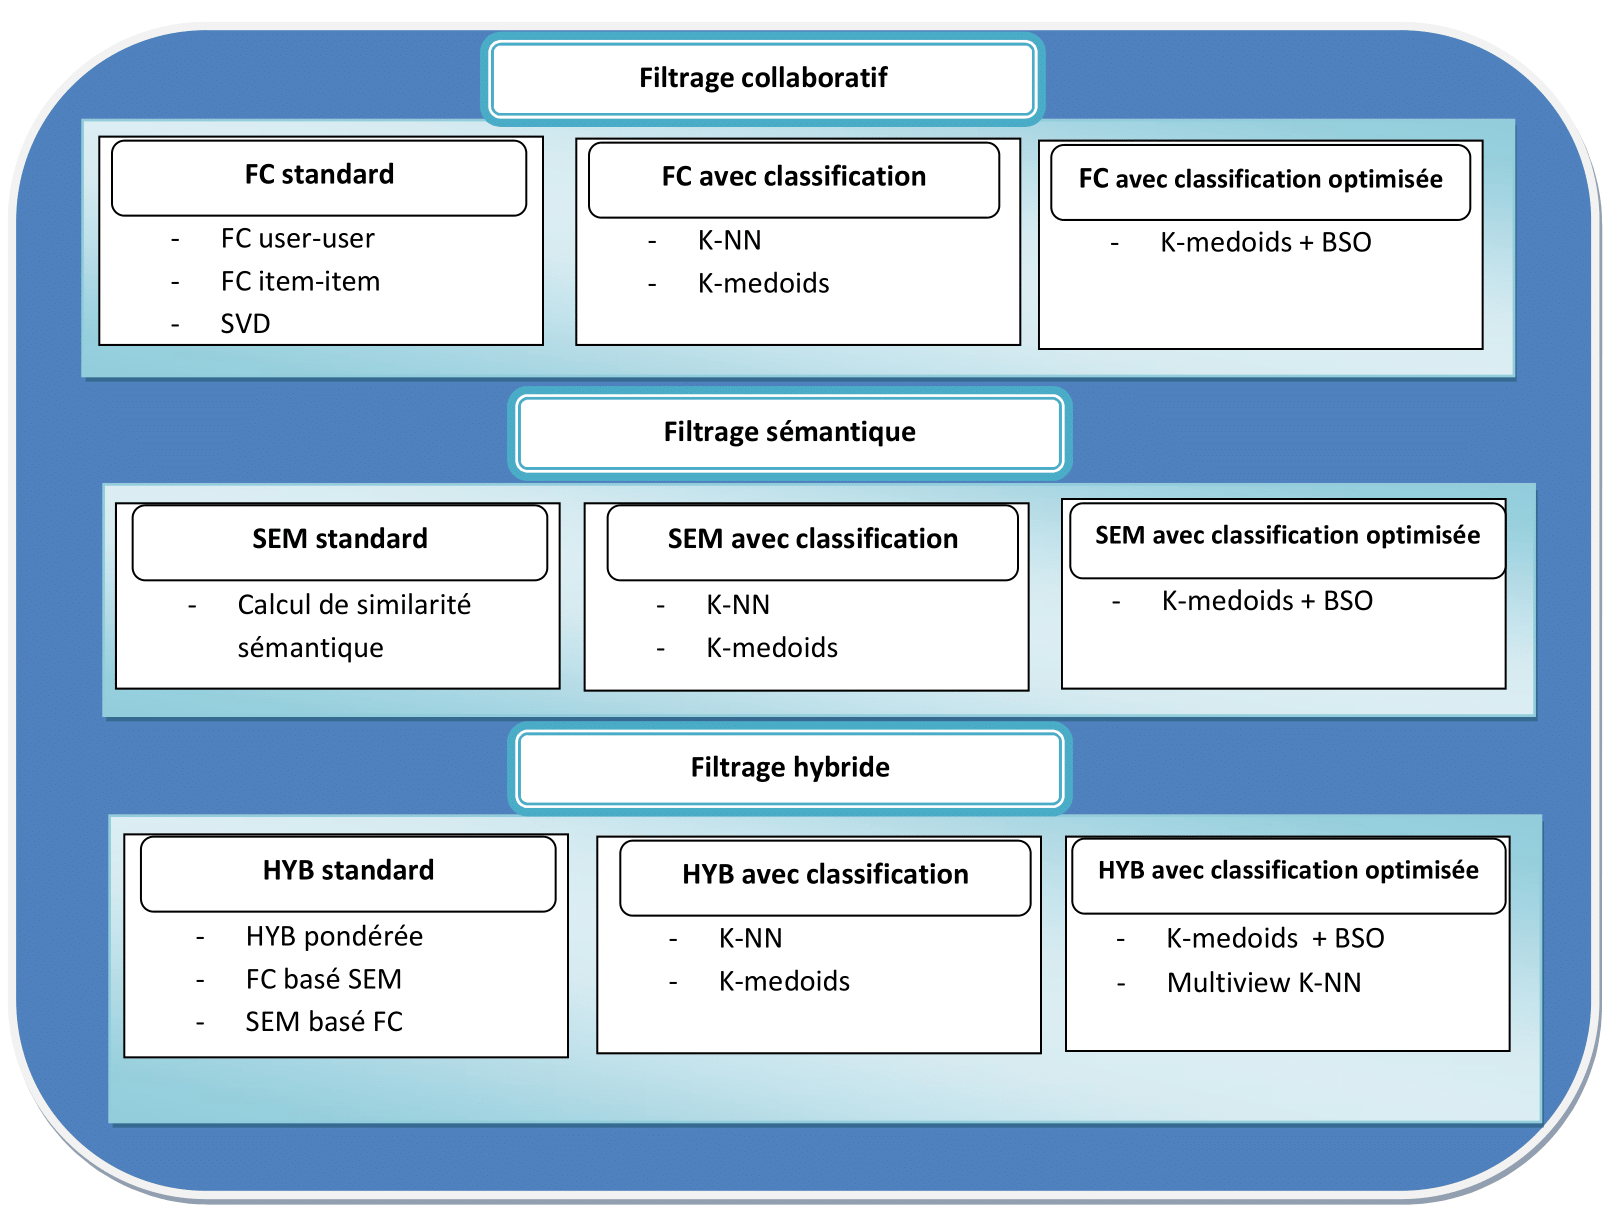
\includegraphics[width=\textwidth]{shema.png}
	\caption{Description générale de notre système de recommandation}
	\label{fig:shema}
\end{figure}

\section{Filtrage sans classification}
\subsection{Filtrage collaboratif}
Nous avons implémenté le filtrage collaboratif user-user,item-item, et une baseline qui est SVD.
\begin{enumerate}[nosep,label=\textbf{\arabic*)}]
	%%  \setcounter{enumi}{4}
	\item \textbf{Filtrage collaboratif standard}
\end{enumerate}\myparagraph{FC user-user}L'idée principale du FC user-user est d'utiliser la matrice d'usage pour déterminer les meilleurs voisins d'un utilisateur (parcours selon les lignes de la matrice), comme expliqué précédemment dans le chapitre 1. Le filtrage collaboratif passe par deux étapes, la première est le calcule de similarité et la détermination des voisins des utilisateurs, la deuxième consiste à effectuer la prédiction.

L'algorithme 1 ci-dessous décrit le FC basé user-user.

 \begin{algorithm}[H]
	\caption{FC}\label{FCUSERUSER}
	\hspace*{\algorithmicindent} \\
	\hspace*{\algorithmicindent} \textbf{Entrée:} Matrice{\_}usage, Seuil ;\\
	\hspace*{\algorithmicindent} \textbf{Sortie:} Ensemble de voisins de chaque utilisateur ;\\\\
	\hspace*{\algorithmicindent}\textbf{ Début:}
	\begin{itemize}
		
		\item []\textbf{Pour} Chaque \textit{utilisateur} de \textit{Matrice{\_}usage} \textbf{faire:} 
		   \begin{itemize}
		   	\item [] Calculer la distance entre cet utilisateur et tout les autres utilisateurs ;
		   	\item [] \textbf{Si:} distance  <= seuil \textbf{Alors} insérer cet utilisateur dans la table voisins du l'utilisateur en cours  \textbf{Fsi ;}
		   \end{itemize}
	   \item []\textbf{Fait ;} 
	
	\end{itemize}
	\hspace*{\algorithmicindent}\textbf{ Fin.}
\end{algorithm} 

\begin{itemize}
	\item \textbf{Seuil:} Nous déterminons le meilleur seuil pour le FC en évaluant les seuils générés à partir de la formule suivante:
	\begin{equation}
	Seuil=\frac{Min(matrice) + Max(matrice)}{10}
	\end{equation}
	Où Min() (respectivement Max()) est une fonction qui retourne la valeur minimum (respectivement maximum) de la matrice.
	À l'issue de l'application de cette formule nous obtenons dix seuils à tester, et nous choisirons celui qui nous donnera les meilleures prédictions. 
\end{itemize}

\begin{itemize}
	\item [-] \textbf{Complexité de l'algorithme}:
	\begin{itemize}
		\item [-] $n$: nombre d'utilisateurs.
		\item [-] Nous effectuons $n$ itérations pour calculer les voisins de chaque utilisateur.
	\end{itemize}
	\item [-] Donc la complexité de FC = $O(n)$
\end{itemize}


\myparagraph{FC item-item}
Comme pour le FC user-user, on détermine les voisins les plus proches des items avec la matrice d'usage mais cette fois-ci selon un parcours colonne par colonne.
\myparagraph {SVD (Singular Value decomposition)}
Dans le contexte des systèmes de recommandation, SVD est utilisée comme algorithme de filtrage collaboratif pour capturer la similarité entre les utilisateurs et les items en extrayant les caractéristiques cachées qu' utilisateur ou un item  possède et ainsi les faire correspondre selon leurs caractéristiques. 
Par exemple, pour les films, l'une des caractéristiques peut  être le genre auquel le film appartient comme comédie, horreur ou les deux en même temps et pour un utilisateur s'il a un caractère sérieux ou drôle ...ect, (voir figure ~\ref{fig:exemplefeatures}). 
Donc nous effectuons une décomposition en valeurs singulières pour extraire ces caractéristiques et avoir la meilleure décomposition de la matrice d'usage qui permet de prédire les ratings des items non encore évalués par les utilisateurs, souvent la métrique erreur racine moyenne (RMSE) est utilisée pour savoir si la décomposition et bonne ou pas(plus RMSE et bas mieux les performances et la prédiction est meilleure), on précise que nous prenons en compte que les ratings qu'on possède lors de la prédiction dans le calcul d'erreur.

SVD est effectué comme indiqué dans la figure \ref{fig:svd} ci-dessous.

\begin{figure}[H]
	\centering
	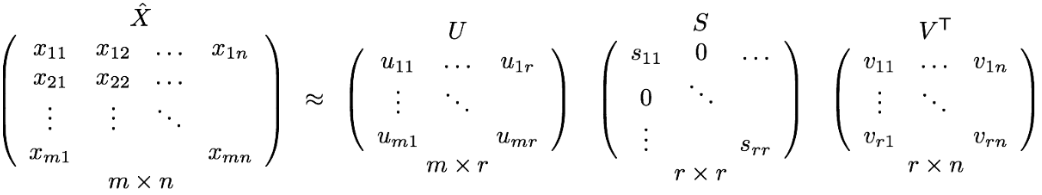
\includegraphics[width=\textwidth]{svd.png}
	\caption{Formule SVD}
	\label{fig:svd}
\end{figure}
Où:
\begin{itemize}
	\item  X: désigne la matrice d'utilité.
	\item  U: matrice singulière gauche, représentant la relation entre les utilisateurs et leurs caractéristiques.
	\item  S: matrice diagonale décrivant la force de chaque caractéristique.
	\item  V: matrice transposée singulière droite indiquant la similitude entre les items et leurs caractéristiques.
\end{itemize}



\begin{figure}[H]
	\centering
	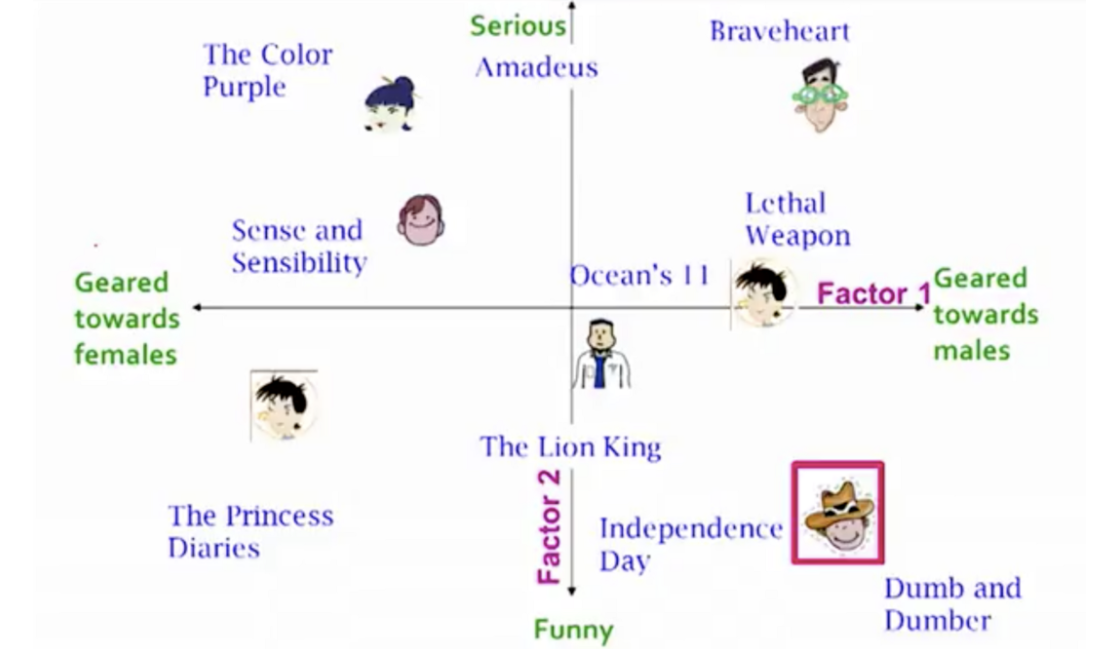
\includegraphics[width=\textwidth]{exemplefeatures.png}
	\caption{Exemple des caractéristiques d'un user \cite{ref31}}
	\label{fig:exemplefeatures}
\end{figure}

La figure \ref{fig:exemplesvd} ci-dessous montre un exemple de SVD

\begin{figure}[H]
	\centering
	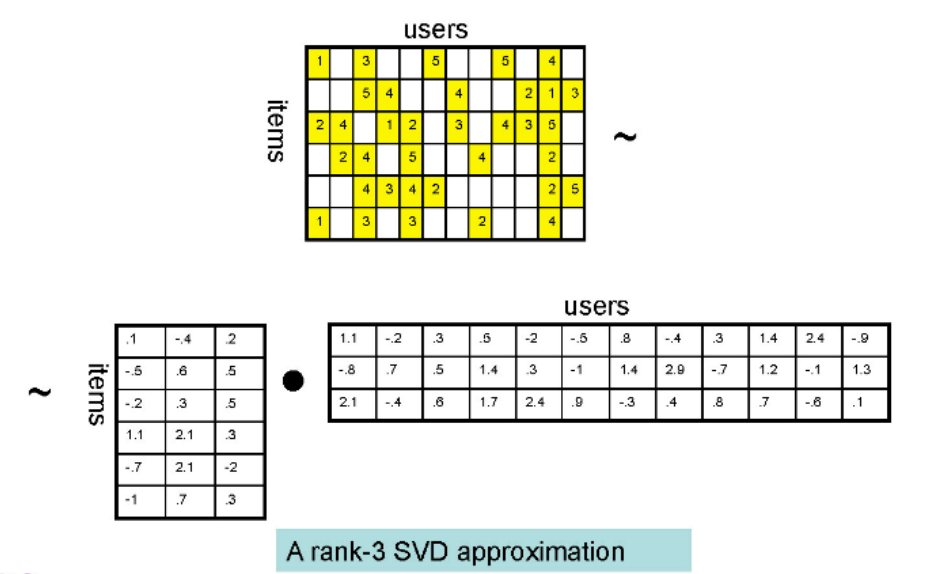
\includegraphics[width=\textwidth]{exempleofSVD.png}
	\caption{Exemple de Singular Value decomposition \cite{ref31}}
	\label{fig:exemplesvd}
\end{figure}
\myparagraph{Calcul de prédiction et distance pour le filtrage collaboratif}
Pour chaque algorithme FC cité précédemment, nous avons utilisé la formule de Pearson afin de calculer la distance entre les utilisateurs et les items, comme suit: 
\begin{itemize}
\item Calcul distance entre utilisateur:\\
Pour le calcul de distance entre deux utilisateurs u et v, la corrélation de Pearson est donnée par la formule suivante :
\begin{equation}\label{key21}
pearson(u,v)= 1 - \frac{\sum_{i \in I} (r_{u,i}-\bar{r}_{u}).(r_{v,i}-\bar{r}_{v})}{\sqrt{\sum_{i \in I} (r_{u,i}-\bar{r}_{u})^{2}.(r_{v,i}-\bar{r}_{v})^{2}}}
\end{equation}

où :
\begin{itemize}
	\item r $_{u,i}$ : est l'estimation de l'utilisateur u sur l’item i.
	\item r $_{v,i}$ : est l'estimation de l'utilisateur v sur l’item i.
	\item $\bar{r}_{u}$ : est la moyenne de toutes les notes de l'utilisateur u. 
	\item $\bar{r}_{v}$ : est la moyenne de toutes les notes de l'utilisateur v.
\end{itemize}

La distance est interprétée comme suit:

\begin{itemize}
	\item Si Pearson(u,v) = 0 alors les utilisateurs u et v sont parfaitement identiques.
	\item Si Pearson(u,v) = 1 alors les utilisateurs u et v ne sont pas corrélés. 
	\item Si 0 < Pearson(u,v) < 1  alors les utilisateurs u et v sont corrélés positivement (proches) et la distance représente le degrés de corrélation. 
	\item Si 1 < Pearson(u,v) < 2  alors les utilisateurs u et v sont corrélés négativement (loin) et la distance représente le degrés de corrélation. 
	\item Si Pearson(u,v) = 2 alors les utilisateurs u et v sont parfaitement opposés.
\end{itemize}

\item Calcul distance entre items:\\
Le calcul de distance entre deux items i et j : la corrélation de Pearson est donnée par la formule suivante :

\begin{equation}
pearson(i,j)= 1 - \frac{\sum_{u \in U} (r_{u,i}-\bar{r}_{i}).(r_{u,j}-\bar{r}_{j})}{\sqrt{\sum_{u \in U} (r_{u,i}-\bar{r}_{i})^{2}.\sum_{u \in U}(r_{u,i}-\bar{r}_{j})^{2}}}
\end{equation}

où :

\begin{itemize}
	\item r$_{u,i}$  : est l’évaluation de l’utilisateur u sur l’item i 
	\item r$_{u,j}$ : est l’évaluation de l’utilisateur u sur l’item j
	\item $\bar{r}_{i}$ : est la moyenne des évaluations de l’item i par les utilisateurs.
	\item $\bar{r}_{j}$ : : est la moyenne des évaluations de l’item j par les utilisateurs.
\end{itemize}
 
 
La distance est interprétée comme suit:
 
 \begin{itemize}
 	\item Si Pearson(i,j) = 0 alors les item i et j sont parfaitement identiques.
 	\item Si Pearson(i,j) = 1 alors les item i et j ne sont pas corrélés. 
 	\item Si 0 < Pearson(i,j) < 1  alors les item i et j  sont corrélés positivement (proches) et la distance représente le degrés de corrélation. 
 	\item Si 1 < Pearson(i,j) < 2  alors les item i et j sont corrélés négativement (loin) et la distance représente le degrés de corrélation. 
 	\item Si Pearson(i,j) = 2 alors les item i et j  sont parfaitement opposés.
 \end{itemize}


Pour la prédiction des valeurs des évaluations (ratings) des items non encore évalués, nous avons utilisé la formule de la somme pondérée:


\begin{equation}
pred(u_{i},i_{k})=\bar{r(u_{i})} + \frac{\sum_{u_{j} \in U_{i}} sim(u_{i},u_{j}).(r_{u_{j,ik}}-\bar{r(u_{j})})}{\sum_{u_{j} \in U_{i}} sim(u_{i},u_{j})}
\end{equation}

Où: 
\begin{itemize}
	\item sim(u$_{i}$,u$_{j}$) : est la mesure de similarité entre un utilisateur u$_{i}$ et son voisin u$_{j}$, tel que u$_{j}$ $\in$ U$_{i}$.
	\item $\bar{r}_{i}$ : est la moyenne des évaluations de l’item i par les utilisateurs.
	\item $\bar{r}_{j}$ : est la moyenne des évaluations de l’item j par les utilisateurs.
	
\end{itemize}
\end{itemize}
\subsection{Filtrage sémantique standard}
Ce type de filtrage utilise la notion sémantique pour déterminer les profils des utilisateurs qui sont similaires. Comme pour le filtrage collaboratif, le filtrage sémantique passe par deux étapes le calcule de similarité entre utilisateurs ensuite la prédication des ratings sur les items non évalués.

Pour déterminer si deux profils d'utilisateurs sont similaires du point de vue sémantique, nous nous intéressons aux items que les deux utilisateurs ont bien notés afin d'identifier les catégories qui sont susceptibles de les intéresser et donc par la suite leur recommander des items de catégories identiques ou similaires. 

C'est à partir de la catégorie d'un item que nous allons extraire l'information sémantique, pour cela nous disposons d'une matrice \textit{item-catégorie} qui contient pour chaque item donné la catégorie à laquelle il appartient.
Un item peut appartenir à plusieurs catégories en même temps, comme le montre la figure \ref{fig:cat} ci-dessous:

\begin{figure}[H]
	\centering
	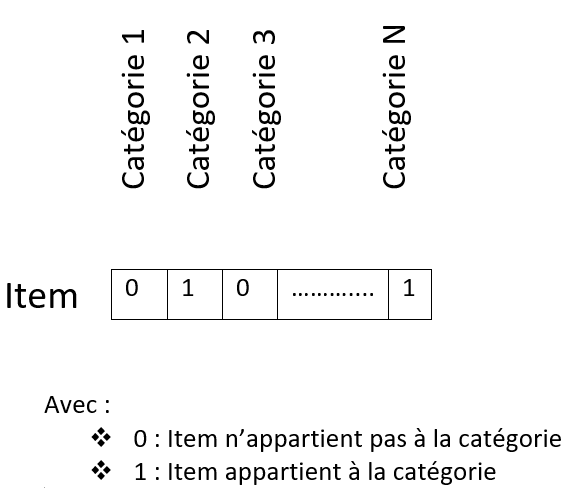
\includegraphics[width=0.60\textwidth]{movie-genre.PNG}
	\caption{Exemple d'une ligne de la matrice \textit{item-catégorie}}
	\label{fig:cat}
\end{figure}

Pour déterminer la similarité sémantique entres les items, nous devons calculer la distance entre ces derniers en se basant sur leurs représentation. Deux cas de figures se présentent à nous:
\begin{itemize}
	\item Les items ne sont pas représentés avec des ontologies: Pour chaque item de la matrice \textit{item-catégorie}, nous appliquons la distance de Jaccard  afin de déterminer les degrés de similarité entre les items et ainsi obtenir une matrice de distance \textit{item-item}. La distance de Jaccard est comprise entre $[0;1]$ et a la propriété d'être égale à 0 quand les items sont différents et 1 quand ils sont identiques et est calculée comme suit:
	
	\begin{equation}
	\displaystyle\text{J}(A,B) = 1 - \frac{|A\cap B|}{|A| + |B| -|A \cup B|} = 1 - \frac{\sum a_{i} * b_{i}}{\sum a_{i}^{2} + \sum b_{i}^{2} - \sum a_{i} * b_{i}}
	\end{equation}
	
	Où:
	\begin{itemize}
		\item $A$ et $B$: sont deux items,
		\item $a_{i}$, $b_{i}$: peuvent être soit 0 ou 1, ils indiquent l'appartenance ou non de l'item $A$ (respectivement $B$) à un une catégorie ${i}$ .
	\end{itemize}

\item Les items sont représentés avec des ontologies: Pour chaque item de la matrice \textit{item-catégorie}, nous appliquons la distance de Wu et Palmer  afin de déterminer les degrés de similarité entre les items et ainsi obtenir une matrice de distance \textit{item-item}. La distance de Wu et Palmer est comprise entre $[0;1]$. Si deux concepts sont identique la distance est égale à zéro et s'ils sont opposés elle est égale à un, et est calculée comme suit:

\begin{equation}
Dist_{WP}= 1 - \frac{ (2*N)}{(N_{1}+N_{2}+2*N)}
\end{equation}
Où:
\begin{itemize}
	\item $C1$ et $C2$: sont deux concepts.
	\item $N1$ et $N2$: la distance  séparant C1 et C2 du nœud racine.
	\item $N$: distance séparant l'ancêtre commun le plus proche de C1 et C2 du nœud racine.
\end{itemize}
\end{itemize}



\begin{figure}[H]
	\centering
	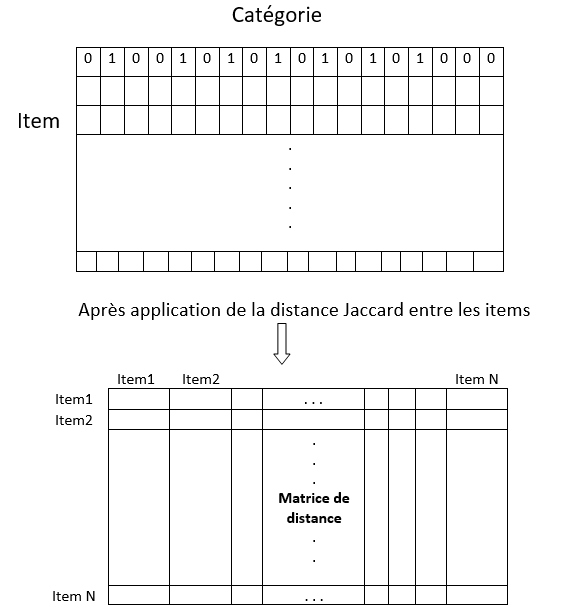
\includegraphics[width=\textwidth]{movie-movie-distance.PNG}
	\caption{Génération de la matrice de distance\textit{ item-item}}
\end{figure}

Après avoir obtenu la matrice distance\textit{ item-item} nous appliquons la formule de distance d'intérêt pour calculer la distance entre les utilisateurs de la matrice d'usage et ainsi obtenir la matrice de distance \textit{user-user} comme suit: 



\begin{equation}
d_{interest}(u,v) = \frac{\sum _{x \in X}n_{x} min_{y \in Y} d_{x,p} (x,y) + \sum_{y \in Y} n_{y} min_{x \in X} d_{w,p} (x,y)} {\sum _{x \in X} n_{x} + \sum _{y \in Y} n_{y}}
\end{equation}

Où: X (respectivement Y) sont les deux catégorie que u (respectivement v) a revu.



\begin{figure}[H]
	\centering
	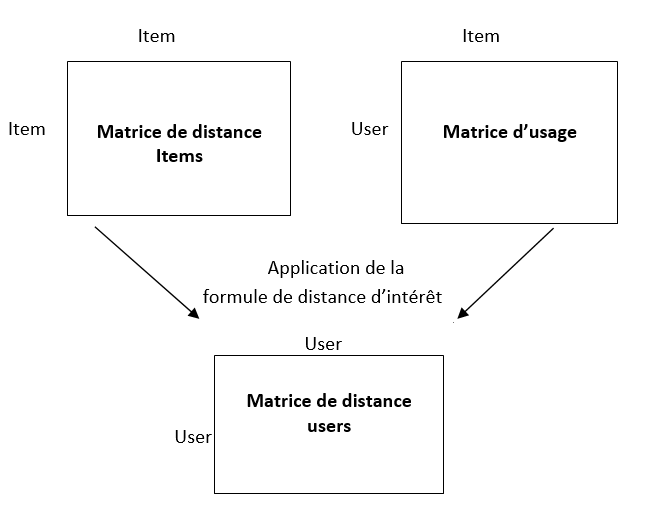
\includegraphics[width=0.8\textwidth]{user-user-interet.PNG}
	\caption{Génération de la matrice de distance \textit{user-user}}
\end{figure}

À partir de la matrice distancée \textit{user-user} nous pouvons déterminer à présent les voisins d'un utilisateur donné en appliquant l'algorithme suivant:

 \begin{algorithm}[H]
	\caption{Filtrage sémantique}
	\hspace*{\algorithmicindent} \\
	\hspace*{\algorithmicindent} \textbf{Entrée:} Matrice de distance user-user, Seuil;\\
	\hspace*{\algorithmicindent} \textbf{Sortie:} Ensemble de voisins de chaque utilisateur \\\\
	\hspace*{\algorithmicindent}\textbf{ Début:}
	\begin{itemize}
		
		\item []\textbf{Pour} Chaque \textit{utilisateur{\_}i} de \textit{matrice{\_}distance} \textbf{faire:} 
		\begin{itemize}
		\item []\textbf{Pour} Chaque \textit{distance{\_}j} de \textit{utilisateur{\_}i} \textbf{faire:} 
		\begin{itemize}
				\item [] /*récupérer l'indice de la colonne, qui représente l'indice du voisin en cours de traitement*/
			\item [] utilisateur{\_}j  $\leftarrow$ indice(distance{\_}j) 
			
			\item [] \textbf{Si:} \textit{distance{\_}j}  <= Seuil \textbf{Alors} insérer \textit{utilisateur{\_}j}  dans la table voisins du l'\textit{utilisateur{\_}i }\textbf{Fsi;}
		\end{itemize}
	
\item []  \textbf{Fait;}
\end{itemize}
\item []  \textbf{Fait;}
	\end{itemize}
	\hspace*{\algorithmicindent}\textbf{ Fin.}
\end{algorithm} 

\begin{itemize}
	\item \textbf{Seuil:} Le seuil est calculé de la même façon que pour le FC (voir seuil dans la partie FC).
\end{itemize}

\begin{itemize}
	\item [-] \textbf{Complexité de l'algorithme}:
	\begin{itemize}
		\item [-] $n$: nombre d'utilisateurs.
		\item [-] $n^2$: taille de la matrice de distance carré.
		\item [-] À chaque itération on fait un parcours de $n^2$ (taille de la matrice de distance).
	\end{itemize}
\item [-]  Donc la complexité du filtrage sémantique = $O(n^2)$
\end{itemize}

\myparagraph{Calcul de prédiction pour le filtrage sémantique}
Pour la prédiction des valeurs des ratings sur les items non encore évalués, nous avons utilisé la formule de la somme pondérée citée précédemment.

\subsection{Filtrage hybride}
Dans cette partie, nous allons détailler trois méthodes d'hybridation que nous avons implémentées entre les 2 types de filtrage déjà réalisés précédemment (sémantique, collaboratif), et qui sont:

\begin{itemize}
	\item Filtrage collaboratif hybride pondéré.
	\item Filtrage collaboratif basé sémantique.
	\item Filtrage sémantique basé collaboratif.
	
\end{itemize}

Pour chaque type d'hybridation conçu, les deux matrices de distance collaboratif (user-user, item-item) et sémantique jouent un rôle très important et sont calculées de la sorte:

\begin{itemize}
\item Matrice distance du filtrage collaboratif: 

Nous appliquons la formule Pearson pour calculer la distance d'un utilisateur avec le reste des utilisateurs de la  matrice d'usage et nous stockons les valeurs des distances dans une matrice comme le montre la figure \ref{fig:distuser} suivante: 

	\begin{figure}[H]
		\centering
		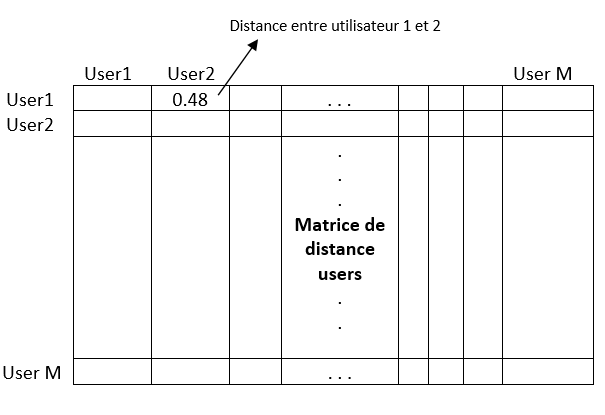
\includegraphics[width=0.80\textwidth]{matUserUSer.PNG}
		\caption{Matrice de distance user-user}
		\label{fig:distuser}
	\end{figure}

	\item  Matrice distance du filtrage sémantique: (voir explication dans la partie filtrage sémantique standard.)
\end{itemize}

\begin{enumerate}[nosep,label=\textbf{\arabic*)}]
	%%  \setcounter{enumi}{4}
	\item \textbf{Filtrage hybride pondéré}
\end{enumerate}\mbox{}\indent 
L'algorithme de filtrage hybride pondéré associe à chaque matrice de distance collaborative et sémantique respectivement un poids $\alpha$ et $\beta$ qui représentent les degrés d'importance de chaque type de recommandation (voir figure \ref{fig:alpha}) avec:
\begin{itemize}
	\item  $0.1 =< \alpha =< 0.9$
	\item  $\beta = 1 - Alpha$ 
	\item 	$\alpha + \beta = 1$
\end{itemize}

\begin{figure}[H]
	\centering
	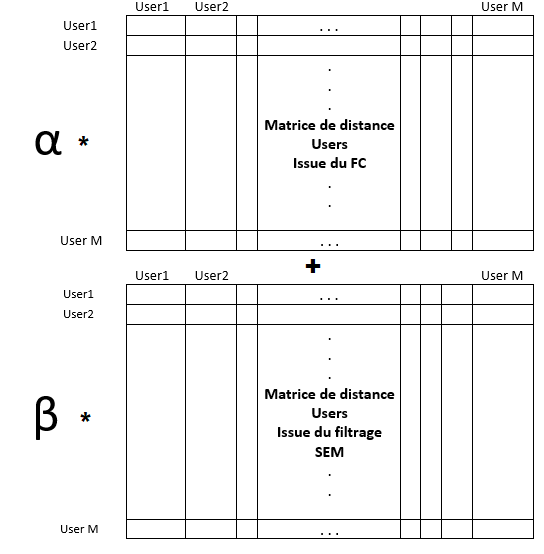
\includegraphics[width=0.9\textwidth]{hybpondere.PNG}
	\caption{Pondération des matrices de distances}
	\label{fig:alpha}
	
\end{figure}

Nous utilisons une boucle, dans laquelle nous augmentons la valeur de $\alpha$ de 0.1, et nous affectons à $\beta$ la valeur $1 - \alpha$, puis nous multiplions la matrice de distance du filtrage collaboratif par $\alpha$ et la matrice de distance du filtrage sémantique par $\beta$, nous évaluons par la suite les prédictions générées à partir de ces deux matrices, nous répétons ce processus jusqu'à ce que nous obtenons les meilleures valeurs possibles pour $\alpha$ et $\beta$ qui permettes d'accorder l'importance adéquate aux filtrages collaboratif et sémantique.

 \begin{algorithm}[H]
	\caption{Filtrage hybride pondéré}\label{HP}
	\hspace*{\algorithmicindent} \textbf{Entrée:}
	 \begin{itemize}
	\item [] Matrice{\_}distance{\_}FC: Matrice de distance du FC user-user , 
	\item [] Matrice{\_}distance{\_}SEM: Matrice de distance du filtrage sémantique user-user,
	\item [] Seuil{\_}Voisin: le seuil d'acceptation d'un voisin ;
	\end{itemize}
	\hspace*{\algorithmicindent} \textbf{Sortie:} 
	\begin{itemize}
	\item [] Ensemble de voisins pour chaque utilisateur selon meilleur poids Alpha ; 
	
	
	\end{itemize}
	
	\hspace*{\algorithmicindent}\textbf{ Début:}
	\begin{itemize}
		
		\item [] Alpha $\leftarrow$ 0.1 ;
		\item [] Beta $\leftarrow$ 1 - Alpha ;
		\item [] Best{\_}evaluation $\leftarrow$ Float(Inf) ;
		\item [] BestAlhpa $\leftarrow$ Float(Inf) ;
		\item []\textbf{Tant que } \textit{Beta >= 0.1}  \textbf{faire :} 
		\begin{itemize}
			
			\item [] AlphaMatrice $\leftarrow$  matrice{\_}distance{\_}FC * Alpha ;
			\item []Beta $\leftarrow$ 1 - Alpha ;
			\item [] BetaMatrice $\leftarrow$  matrice{\_}distance{\_}SEM * Beta ;
			\item  [] SommeMatrices $\leftarrow$  AphaMatrice +  BetaMatrice ;
			\item  [] Voisins{\_}users  $\leftarrow$ Voisin (SommeMatrices , Seuil{\_}Voisin) ;
			\item [] tableau{\_}prediciton $\leftarrow$  Prediction (usage{\_}matrice , Voisins{\_}users ) ;
			\item [] evaluation $\leftarrow$ Evaluation (tableau{\_}prediciton , reelles{\_}valeurs) ;
			\item [] \textbf{Si:} Best{\_}evaluation  >=  evaluation \textbf{Alors} 
			\begin{itemize}
				\item [] 	Swap (Best{\_}evaluation, evaluation) ;
				\item [] 	BestAlpha $\leftarrow$ valeurAlpha ;
			\end{itemize}	
				\item [] \textbf{Fsi ;}
				\item [] Alpha $\leftarrow$ Alpha - 0.1 ;
					
		\item [] \textbf{Fait ;} 
		\end{itemize}
		\item [] \textbf{Fait ;} 
	\end{itemize}
	\hspace*{\algorithmicindent}\textbf{ Fin.}
\end{algorithm} 

Où:
\begin{itemize}
	\item Voisins: Fonction qui calcule les voisins pour chaque utilisateur à partir d'un seuil et de la matrice de distance entre utilisateurs.
	\item Prediction: Fonction qui effectue les prédictions des items non évalués pour chaque utilisateur.
	\item Evaluation: Fonction qui calcule la qualité d'une prédiction effectuée. 
\end{itemize}

\begin{itemize}
	\item [-] \textbf{Complexité de l'algorithme}:
	\begin{itemize}
		\item [-] $n$: nombre d'utilisateurs.
		\item [-] $n^2$: taille de la matrice de distance carré.
		\item [-] Nous avons neuf itérations (de 0.1 jusqu'à 0.9).
		\item [-] À chaque itération on fait un parcours de $n^2$ (taille de la matrice de distance).
	\end{itemize}
	\item [-]  Donc la complexité du filtrage hybride pondéré = $O(9*n^2)$
\end{itemize}


\begin{enumerate}[nosep,label=\textbf{\arabic*)}]
	 \setcounter{enumi}{1}
	\item \textbf{Filtrage hybride sémantique basé collaboratif}
\end{enumerate}\mbox{}\indent Le filtrage sémantique standard décrit précédemment, utilise une matrice de distance entre les items qui est calculée avec la formule Jaccard, ici nous allons la remplacer avec la matrice de distance items issue du filtrage collaboratif (voir figure \ref{fig:semfc}) en utilisant la formule Pearson comme suit:
\begin{itemize}
	\item [-]Soit deux items i et j : la corrélation de Pearson est donnée par la formule suivante :
\end{itemize}
\begin{equation}
pearson(i,j)=\frac{\sum_{u \in U} (r_{u,i}-\bar{r}_{i}).(r_{u,j}-\bar{r}_{j})}{\sqrt{\sum_{u \in U} (r_{u,i}-\bar{r}_{i})^{2}.\sum_{u \in U}(r_{u,i}-\bar{r}_{j})^{2}}}
\end{equation}

Où:

\begin{itemize}
	\item r$_{u,i}$  : est l’évaluation de l’utilisateur u sur l’item i 
	\item r$_{u,j}$ : est l’évaluation de l’utilisateur u sur l’item j
	\item $\bar{r}_{i}$ : est la moyenne des évaluations de l’item i par les utilisateurs.
	\item $\bar{r}_{j}$ : est la moyenne des évaluations de l’item j par les utilisateurs.
\end{itemize}

\begin{figure}[H]
	\centering
	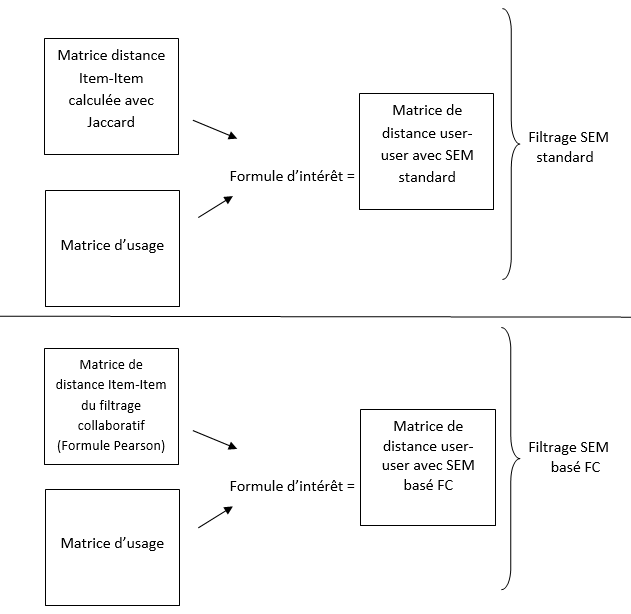
\includegraphics[width=\textwidth]{differance-entre-stand-sembasefc.PNG}
	\caption{Différence entre sémantique standard et sémantique basé collaboratif}
	\label{fig:semfc}
\end{figure}
\textbf{Remarque:} Après avoir passer en entrée la matrice de distance entre les items issue du FC, le même algorithme du filtrage sémantique est utilisé pour effectuer le filtrage sémantique basé collaboratif.
\myparagraph{Calcul de prédiction et distance pour le filtrage hybride sémantique basé collaboratif }
Pour la prédiction des valeurs des ratings sur les items non encore évalués, nous avons utilisé la formule de la somme pondérée citée précédemment.
Quant au calcule de distance entre utilisateurs elle s'effectue comme montré dans le filtrage sémantique en utilisant la même formule de calcul de distance d'intérêt (Formule 3.5). \\


\begin{enumerate}[nosep,label=\textbf{\arabic*)}]
	\setcounter{enumi}{2}
	\item \textbf{Filtrage hybride collaboratif basé sémantique}
\end{enumerate}\mbox{}\indent \iffalse  Dans le filtrage collaboratif, la matrice de distance est calculée avec la formule Pearson, qui donne une distance comprise entre [-1,1], si la distance est égale à 0 cela signifie qu'on ne sait pas si les deux utilisateurs sont corrélés ou pas et ça nous mène à un cas d'indétermination, donc pour y remédier on utilise la matrice de distance du filtrage sémantique dans le cas ou on trouve dans la matrice de distance du filtrage collaboratif \textit{user-user} des distances égalent à 0.
\fi Dans ce filtrage nous effectuons une séléction des voisins d'un utilisateur en utilisant les deux matrices de distance du FC et du filtrage sémantique.
Pour deux utilisateur A et B, B est considéré comme voisin de A ssi :\\
$\min( DFC(A,B) , DFSEM(A,B) ) <= seuil$
\\
Où:
\begin{itemize}
	\item DFC: distance ente utilisateur A et B selon le filtrage collaboratif.
	\item DFSEM: distance ente utilisateur A et B selon le filtrage sémantique.
	\item seuil: seuil d'acceptation d'un voisin pour un utilisateur donnée.
\end{itemize}

\begin{figure}[H]
	\centering
	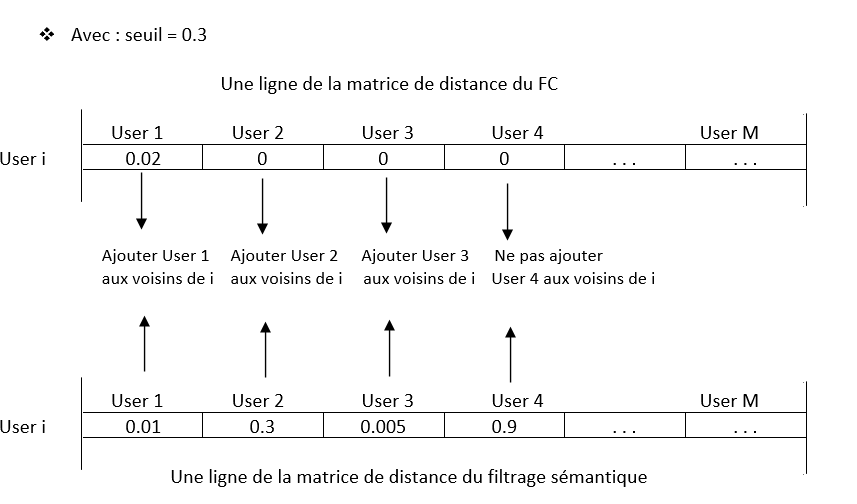
\includegraphics[width=\textwidth]{fcbasesem.PNG}
	\caption{Exemple de filtrage collaboratif-sémantique}
\end{figure}
\iffalse 
 \begin{algorithm}[H]
	\caption{Filtrage sémantique basé collaboratif}\label{sembasécol}
	\hspace*{\algorithmicindent} \\
	\hspace*{\algorithmicindent} \textbf{Entrée:} \begin{itemize}
		\item [] Matrice{\_}distance{\_}FC: Matrice de distance du FC user-user , 
		\item [] Matrice{\_}distance{\_}SEM: Matrice de distance du filtrage sémantique user-user;
		\item []  Seuil{\_}Voisin: le seuil d'acceptation d'un voisin ;
	\end{itemize}
	\hspace*{\algorithmicindent} \textbf{Sortie:} 
	\begin{itemize}
		\item [] Ensemble de voisins de chaque utilisateur
	\end{itemize}

	\hspace*{\algorithmicindent}\textbf{ Début:}
	
	\begin{itemize}
		\item [] \textbf{Pour} Chaque \textit{utilisateur{\_}i} de \textit{ Matrice{\_}distance{\_}FC} \textbf{faire:} 
	
		\begin{itemize}
		\item [] \textbf{Pour} Chaque \textit{distance{\_}j} de \textit{utilisateur{\_}i} \textbf{faire:} 
		\begin{itemize}
		\item [] /*récupérer l'indice de la colonne, qui représente l'indice du voisin en cours de traitement*/
		\item [] utilisateur{\_}j  $\leftarrow$ indice(distance{\_}j) 
		\item [] \textbf{Si:} distance{\_}j ==  0 \textbf{Alors} 
		\begin{itemize}
		\item [] distance{\_}j $\leftarrow$ Matrice{\_}distance{\_}SEM [ \textit{utilisateur{\_}i,utilisateur{\_}j }] \textbf{Fsi;}
		
		\end{itemize}
		\item [] \textbf{Si:} distance  <= Seuil \textbf{Alors} insérer utilisateur{\_}j  dans la table voisins du l'utilisateur{\_}i \textbf{Fsi;}
		\end{itemize}
	

		\end{itemize}
	\end{itemize}
		
	\hspace*{\algorithmicindent}\textbf{ Fin.}
\end{algorithm} 
\fi


\begin{algorithm}[H]
	\caption{Filtrage hybride collaboratif basé sémantique}
	\hspace*{\algorithmicindent} \\
	\hspace*{\algorithmicindent} \textbf{Entrée:} \begin{itemize}
		\item [] Matrice{\_}distance{\_}FC: Matrice de distance du FC user-user , 
		\item [] Matrice{\_}distance{\_}SEM: Matrice de distance du filtrage sémantique user-user;
		\item []  Seuil{\_}Voisin: le seuil d'acceptation d'un voisin ;
	\end{itemize}
	\hspace*{\algorithmicindent} \textbf{Sortie:} 
	\begin{itemize}
		\item [] Ensemble de voisins de chaque utilisateur ;
	\end{itemize}
	
	\hspace*{\algorithmicindent}\textbf{ Début:}


	
	\begin{itemize}
	\item []	Matrice{\_}distance $\leftarrow$ Min ( Matrice{\_}distance{\_}FC , Matrice{\_}distance{\_}SEM ) ;
		
		\item [] \textbf{Pour} Chaque \textit{utilisateur{\_}i} de \textit{ Matrice{\_}distance} \textbf{faire:}
				
		\begin{itemize}
			\item [] \textbf{Pour} Chaque \textit{distance{\_}j} de \textit{utilisateur{\_}i} \textbf{faire:} 
			\begin{itemize}
				\item [] /*récupérer l'indice de la colonne, qui représente l'indice du voisin en cours de traitement*/
				\item [] utilisateur{\_}j  $\leftarrow$ indice(distance{\_}j) 

				\item [] \textbf{Si:} distance{\_}j  <= Seuil \textbf{Alors} insérer utilisateur{\_}j  dans la table voisins du l'utilisateur{\_}i \textbf{Fsi;}
			\end{itemize}
			
			\item []  \textbf{Fait;}
		\end{itemize}
	\item []  \textbf{Fait;}
	\item [] \textbf{ Fin.}
	\end{itemize}
	

\end{algorithm} 

Où:
\begin{itemize}
	\item Min(): Fonction qui prend minimum des distances entre deux matrices et les stocke dans une nouvelle matrice.
\end{itemize}

\begin{itemize}
	\item [-] \textbf{Complexité de l'algorithme}:
	\begin{itemize}
		\item [-] $n$: nombre d'utilisateurs.
		\item [-] $n^2$: taille de la matrice de distance carré.
		\item [-] À chaque itération on fait un parcours de $n^2$ (taille de la matrice de distance).
	\end{itemize}
	\item [-]  Donc la complexité du filtrage collaboratif basé sémantique = $O(n^2)$
\end{itemize}


\section{Filtrage avec classification}
Dans cette partie, nous allons expliquer l'amélioration apportée aux différents filtrages conçus jusqu'à présent en leurs ajoutant une technique de classification, on précise que la matrice de distance que nous allons utiliser pour classifier les utilisateurs est le résultat d'une des variantes du FC, notre choix sera basé sur les tests effectués afin de prendre la meilleure variante, donc nous aurons à choisir entre FC item-item, FC user-user ou SVD. Concernant le FSem nous avons conçu une seule variante par conséquent il n'y aura pas de choix à faire. Enfin, pour le filtrage hybride nous incorporons la classification dans les trois méthodes réalisées (filtrage hybride pondéré, collaboratif basé sémantique et sémantique basé collaboratif.(voir figure \ref{fig:selec})

\begin{figure}[H]
	\centering
	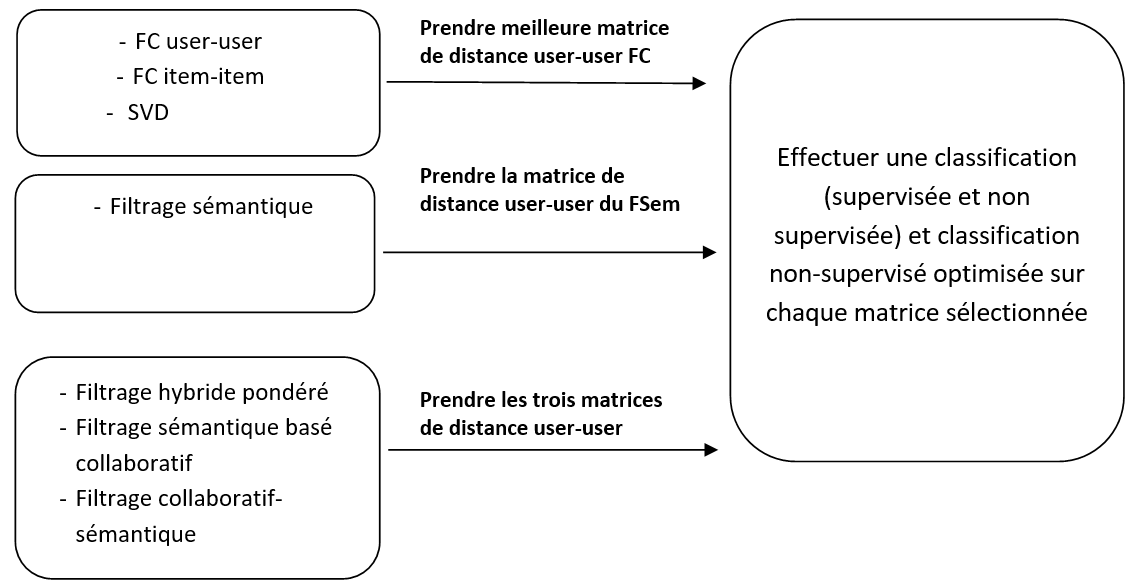
\includegraphics[width=1.1\textwidth]{selectionbestmat.PNG}
	\caption{Sélection des matrices de distance \textit{user-user} pour l'application de la classification}
	\label{fig:selec}
\end{figure}

\subsection{Filtrage avec classification supervisée}
\begin{enumerate}[nosep,label=\textbf{\arabic*)}]
	%%  \setcounter{enumi}{4}
	\item \textbf{K-NN}
\end{enumerate}\mbox{}\indent Comme motionné dans le chapitre 2, K-NN est un algorithme d'apprentissage automatique. Dans notre cas nous l'avons utilisé pour effectuer les prédictions d'un utilisateur donné, en se basant sur ses voisins les plus proches. Nous avons besoin donc des distances entre utilisateurs sous forme de matrice de distance \textit{user-user} issue d'un des type de filtrage et \textit{K} qui est le nombre de voisins à considérer.

Par exemple pour effectuer un filtrage sémantique basé K-NN, il suffit d'envoyer à l'algorithme ci-dessous la matrice de distance \textit{user-user} issue du filtrage sémantique.
Il en est de même pour effectuer:
\begin{itemize}
	\item Filtrage collaboratif basé K-NN.
	\item Filtrage hybride pondéré basé K-NN.
	\item Filtrage collaboratif basé sémantique avec classification K-NN.
	\item Filtrage sémantique basé collaboratif avec  classification K-NN.
\end{itemize}

\begin{algorithm}[H]
	\caption{Filtrage avec classification supervisée (K-NN)}
	\hspace*{\algorithmicindent} \\
	\hspace*{\algorithmicindent} \textbf{Entrée:} \begin{itemize}
		\item [] Matrice{\_}distance{\_}user-user: Matrice de distance issue d'un des types de filtrage , 
		\item []  K: le nombre de voisins à considérer dans les prédictions;
	\end{itemize}
	\hspace*{\algorithmicindent} \textbf{Sortie:} 
	\begin{itemize}
		\item [] Ensemble de K voisins de chaque utilisateur ;
	\end{itemize}
	
	\hspace*{\algorithmicindent}\textbf{ Début:}
	
	\begin{itemize}
		\item [] Voisins[ ] ;/*Liste de listes qui contient les voisins des utilisateurs*/
		\item [] \textbf{Pour} Chaque \textit{utilisateur{\_}i} de \textit{ Matrice{\_}distance{\_}user-user} \textbf{faire:} 
			
			\begin{itemize}
				\item [] /*trier selon l'ordre croissant les distances entre l'utilisateur i et le reste des utilisateur du dataset contenu dans la ligne utilisateur{\_}i */
				\item []	sortedListe $\leftarrow$ Sort(utilisateur{\_}i) ;
			\item []	/*Récupérer les indices des K plus proches voisins de l'utilisateur{\_}i/
				\item [] Voisins[utilisateur{\_}i] $\leftarrow$ Min{\_}K{\_}distance(K,indice(soretedListe)) ;
				
			\end{itemize}
		\end{itemize}
		
		\hspace*{\algorithmicindent}\textbf{ Fin.}
	\end{algorithm} 

\begin{itemize}
	\item [-] \textbf{Complexité de l'algorithme}:
	\begin{itemize}
		\item [-] $n$: nombre d'utilisateurs.
		\item [-] CAAT: complexité approximative de l'algorithme de trie.
		\item [-] À chaque itération on fait un parcours de $n$ (taille de la matrice de distance).
	\end{itemize}
	\item [-]  Donc la complexité du filtrage avec classification supervisée = $O(n*CAAT)$
\end{itemize}
	
\mbox{}
\begin{enumerate}[nosep,label=\textbf{\arabic*)}]
	  \setcounter{enumi}{1}
	\item \textbf{Hybridation mutivues, collaborative et sémantique, basé sur K-NN}
\end{enumerate}\mbox{}\indent Cette approche est inspirée du travail des chercheurs Guibing Guo et al. \cite{ref30}, dans lequel ils effectuent un clustering des utilisateurs en appliquant deux fois consécutives k-medoids (une fois selon la vue similarité et la deuxième fois selon la vue de confiance entre utilisateurs) et par la suite combiner le résultat des deux vues.
Nous avons étudié leur travail et put aboutir à l'idée d'utiliser l'algorithme K-NN selon nos deux vues sémantique et collaboratif.
Le choix de l'algorithme K-NN semble adéquat aux données et informations dont on dispose, de plus c'est un algorithme simple et très utilisé dans la recommandation.

L'idée générale de notre approche est d'effectuer une classification K-NN sur la matrice de distance \textit{user-user} du FC et de prendre K utilisateurs ce qui nous donne une classification selon une première vue, par la suite refaire la même chose sur la matrice de distance \textit{user-user} du filtrage sémantique  pour avoir la deuxième vue, enfin combiner les deux classifications en exécutant K-NN une autre fois sur les K utilisateurs issues de la première classification et de la deuxième (voir figure \ref{fig:knn}).


\begin{figure}[H]
	\centering
	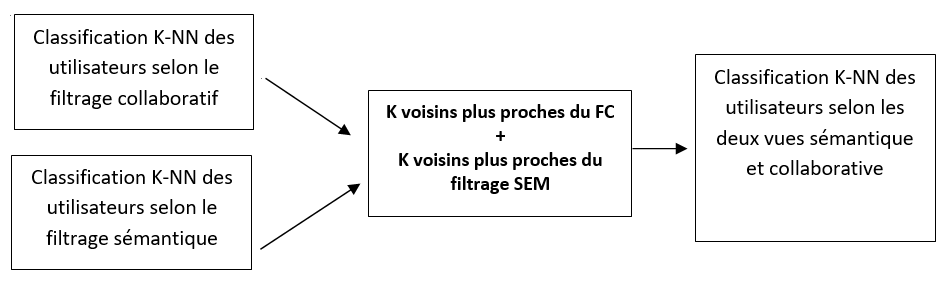
\includegraphics[width=\textwidth]{multiviewknn.PNG}
	\caption{Schéma du filtrage multiview K-NN}
	\label{fig:knn}
\end{figure} 

\begin{algorithm}[H]
	\caption{Filtrage avec multiview (K-NN) Partie 1}
	\hspace*{\algorithmicindent} \\
	\hspace*{\algorithmicindent} \textbf{Entrée:} \begin{itemize}
		\item [] Matrice{\_}distance{\_}user-user{\_}FC: Matrice de distance issue d'un du filtrage collaboratif,
		\item [] Matrice{\_}distance{\_}user-user{\_}SEM: Matrice de distance issue d'un du filtrage sémantique,
		\item []  K: le nombre de voisins à considérer dans les prédictions;
	\end{itemize}
	\hspace*{\algorithmicindent} \textbf{Sortie:} 
	\begin{itemize}
		\item [] Ensemble de K voisins de chaque utilisateur selon les deux vues ;
	\end{itemize}
	
	\hspace*{\algorithmicindent}\textbf{ Début:}
	\hspace*{\algorithmicindent}\\Voisins[ ]{\_}CF ;/*Liste de listes qui contient les voisins des utilisateurs selon filtrage collaboratif*/
	\hspace*{\algorithmicindent}\\ Voisins[ ]{\_}SEM ;/*Liste de listes qui contient les voisins des utilisateurs selon filtrage sémantique*/
\hspace*{\algorithmicindent}\\\textbf{Pour} Chaque \textit{utilisateur{\_}i} de \textit{ Matrice{\_}distance{\_}user-user{\_}CF} \textbf{faire:} 
		
		\begin{itemize}
			\item [] /*trier selon l'ordre croissant les distances entre l'utilisateur i et le reste des utilisateur du dataset contenu dans la ligne utilisateur{\_}i */
			\item []	sortedListe $\leftarrow$ Sort(utilisateur{\_}i) ;
			\item []	/*Récupérer les indices des K plus proches voisins de l'utilisateur{\_}i/
			\item [] Voisins[utilisateur{\_}i]{\_}CF$\leftarrow$ Min{\_}K{\_}distance(K,indice(soretedListe)) ;
			
		\end{itemize}
	
	
	 \textbf{Pour} Chaque \textit{utilisateur{\_}i} de \textit{ Matrice{\_}distance{\_}user-user{\_}SEM} \textbf{faire:} 
	
	\begin{itemize}
		\item [] /*trier selon l'ordre croissant les distances entre l'utilisateur i et le reste des utilisateur du dataset contenu dans la ligne utilisateur{\_}i */
		\item []	sortedListe $\leftarrow$ Sort(utilisateur{\_}i) ;
		\item []	/*Récupérer les indices des K plus proches voisins de l'utilisateur{\_}i/
		\item [] Voisins[utilisateur{\_}i]{\_}SEM$\leftarrow$ Min{\_}K{\_}distance(K,indice(soretedListe)) ;
		
	\end{itemize}

\end{algorithm} 

\setcounter{algorithm}{5}
\begin{algorithm}[H]
\caption{Filtrage avec multiview (K-NN) Partie 2}
/*Fusionner les deux vues*/
\hspace*{\algorithmicindent} \\Voisins[ ]$\leftarrow$ Voisins[utilisateur{\_}i]{\_}SEM + Voisins[utilisateur{\_}i]{\_}CF ;

\textbf{Pour} Chaque \textit{utilisateur{\_}i} de \textit{ Voisins[ ]} \textbf{faire:} 

\begin{itemize}
	\item [] /*trier selon l'ordre croissant les distances entre l'utilisateur i et le reste des utilisateur du dataset contenu dans la ligne utilisateur{\_}i */
	\item []	sortedListe $\leftarrow$ Sort(utilisateur{\_}i) ;
	\item []	/*Récupérer les indices des K plus proches voisins de l'utilisateur{\_}i/
	\item [] Voisins[utilisateur{\_}i]{\_}Multiview $\leftarrow$ Min{\_}K{\_}distance(K,indice(soretedListe)) ;
	
\end{itemize}

\textbf{ Fin.}
\end{algorithm} 
\begin{itemize}
	\item [-] \textbf{Complexité de l'algorithme}:
	\begin{itemize}
		\item [-] $n$: nombre d'utilisateurs.
		\item [-] CAAT: complexité approximative de l'algorithme de trie.
		\item [-] Nous effectuons trois fois l'algorithme K-NN.
		\item [-] À chaque itération on fait un parcours de $n$ (taille de la matrice de distance).
	\end{itemize}
	\item [-]  Donc la complexité du filtrage avec classification supervisée = $O(3*n*CAAT)$
\end{itemize}


\subsection{Filtrage avec classification non supervisée}
\begin{enumerate}[nosep,label=\textbf{\arabic*)}]
	%%\setcounter{enumi}{1}
	\item \textbf{Filtrage basé sur K-medoids}
\end{enumerate}\mbox{}\indent Le principe est d'appliquer l'algorithme K-medoids sur l'ensemble des utilisateurs de manière à construire des clusters qui contiennent des utilisateurs possédant des intérêts similaires, le choix des utilisateurs qui seront considérés comme medoids de départ s'effectue de façon aléatoire.
Les distances entre les utilisateurs sont stockées dans les matrice distance \textit{user-user} issue d'un des type de filtrage.

Par exemple pour effectuer un filtrage sémantique basé K-medoids, il suffit d'envoyer à l'algorithme ci-dessous la matrice de distance \textit{user-user} issue du filtrage sémantique.
Il en est de même pour effectuer:
\begin{itemize}
	\item Filtrage collaboratif basé K-medoids.
	\item Filtrage hybride pondéré basé K-medoids.
	\item Filtrage collaboratif basé sémantique avec clustering K-medoids.
	\item Filtrage sémantique basé collaboratif avec clustering K-medoids.
\end{itemize}


\begin{algorithm}[H]
	\caption{Filtrage avec classification non supervisé  (K-medoids)}
	\hspace*{\algorithmicindent} \\
	\hspace*{\algorithmicindent} \textbf{Entrée:}
		\begin{itemize}
		\item [] Matrice{\_}distance{\_}user-user: Matrice qui contient les distances entre utilisateur issue d'un des types de filtrage , 
		\item [] K: Le nombre de cluster à former ;
		\end{itemize}
		\hspace*{\algorithmicindent} \textbf{Sortie:} 
	\begin{itemize}
		\item [] Clustering des utilisateurs en K cluster ;
	\end{itemize}
	\hspace*{\algorithmicindent}\textbf{ Début:}	
		
		\begin{itemize}
		\item  [] Medoids $\leftarrow$ Choisir les K centres  des clusters : Désigné aléatoirement K indices de la matrice de distances représentant les indices de K utilisateurs ;
		\item [] calculer le cout initial;	

		\item [] \textbf{Pour} Chaque \textit{M-user } de \textit{Medoids} \textbf{faire:}
		\begin{itemize}
			\item [] \textbf{Pour} Chaque \textit{N-user}  de \textit{non-Medoids} \textbf{faire:}
			\begin{itemize}
				\item [] Swap(M,O) ;
				\item [] Distribution(Matrice{\_}distance{\_}user-user, Medoids) ;
				\item [] calculerCout( );
				\item []  \textbf{Si:} le cout de cette itération est supérieure au cout de l'itération précédente \textbf{alors} Undo(M-user,N-user) ; \textbf{Fsi;}	
				\item []  \textbf{Si:} Aucune changement alors arrêter l'algorithme \textbf{Fsi;}			
				
			\end{itemize}
			\item []\textbf{Fait;}
		\end{itemize}
		\item []\textbf{Fait;}
		\end{itemize}

	\hspace*{\algorithmicindent}\textbf{ Fin.}	
\end{algorithm}

Où: 
\begin{itemize}
	\item [-] Swap() : Remplace le medoid M-user par N-user
	\item [-] Undo() : Annule le swap de M-user par N-user
	\item [-] Distribution() : Assigne les utilisateurs au plus proche cluster en utilisant la matrice de distance et les medoids 
	\item [-] Cout() : Fonction objective qui est destinée à être minimisée
\end{itemize}

\begin{equation}
Cout=\min\sum_{c \in C}\sum_{u,v \in c}d(u,v)
\end{equation}

Avec : C l'ensemble des clusters résultant de l'lagorithme k-medoids, u et v deux utilisateurs, v appartient au cluster et u son medoids.

\begin{itemize}
	\item [-] \textbf{Complexité de l'algorithme}:
	\begin{itemize}
		\item [-] $n$: nombre d'utilisateurs.
		\item [-] $k$: nombre de clusters à former.
		\item [-] Nous devons trouver la distance entre chacun des $(n-k)$ points de données k fois pour placer les points de données dans le groupe le plus proche.
		\item [-] Après cela, nous devons remplacer chacun des medoids précédemment supposés par chaque non-medoid et recalculer la distance entre les objets $(n-k)$.
	\end{itemize}
	\item [-]  Donc la complexité du filtrage avec classification non supervisée = $O(k(n-k)^2)$
\end{itemize}


\subsection{Filtrage avec classification non supervisée optimisée}
Comme nous l'avons vu dans le chapitre précédent l'optimisation par colonie d'abeilles manipule un ensemble d'abeilles où chaque abeille correspond à une solution faisable d'un problème donné.
Nous avons décider d'exploiter le mieux possible BSO dans le but d'optimiser le clustering effectué par K-medoids, et ainsi améliorer la qualité des prédictions.

K-medoids commence initialement par des medoids qui sont sélectionnés aléatoirement, en utilisant BSO nous tentons de trouver les meilleurs medoids de départ qui permettent de faire le meilleur partitionnement possible des utilisateurs, et de ne pas effectuer une sélection aléatoire des medoids car nous avons peu de chance de tomber sur de bons medoids.

Cette classification non supervisée optimisée est appliquée pour les différents types de filtrage conçu (FC, FSem et Filtrage hybride) car 
nous faisons appelle à l'algorithme BSO qui lui fait appelle à l'algorithme K-medoids, ce dernier comme vu précédemment (voir Filtrage basé sur K-medoids) à en entrée une matrice de distance issue de l'un des types de filtrages implémentés.\\

\begin{enumerate}[nosep,label=\textbf{\arabic*)}]
	%%\setcounter{enumi}{1}
	\item \textbf{Codification et initialisation de la solution}
\end{enumerate}\mbox{}\indent Afin d'exploiter le mieux possible la métaheuristique et prouver son efficacité il est nécessaire de faire une codification adéquate qui permet de modéliser le problème.
Dans notre cas, chaque partitionnement des users effectué par k-medoids représente une solution, donc chaque abeille correspond à un partitionnement faisable.

La solution est représentée par un vecteur de taille égale au nombre d'utilisateurs à classifier dans un dataset, les indices du vecteur représentent les identificateurs des utilisateurs et chaque case du vecteur peut contenir un 0 ou 1 qui signifient respectivement:
\begin{itemize}
	\item le i ème utilisateur du vecteur solution n'est pas medoid.
	\item le i ème  utilisateur de vecteur solution est medoid.
\end{itemize}

On démarre l'algorithme avec une solution initiale qui est soit aléatoire en remplissant un vecteur de taille N (N = nombre d'utilisateurs) avec 0 et 1, ou une solution qui est le résultat d'un vecteur construit à partir des clusters sorties de l'algorithme K-medoids qui représente un partitionnement des utilisateurs en K clusters.\\

\begin{enumerate}[nosep,label=\textbf{\arabic*)}]
	\setcounter{enumi}{1}
	\item \textbf{Pseudo code de l'algorithme BSO adapté au probléme de recommandation}
\end{enumerate}\mbox{}\indent Le pseudo-code suivant explique le principe de l'algorithme BSO adapté à notre problème. À noter qu'à chaque ajout d'une solution référence on doit vérifier qu'elle n'est pas déjà dans la liste taboue.  


\begin{algorithm}[H]
	\caption{Recommandation avec K-medoids optimisée (BSO) partie 1}
	\hspace*{\algorithmicindent} \textbf{Entrée:}
	\begin{itemize}
		\item [] Matrice{\_}distance{\_}user-user: Matrice qui contient les distances entre utilisateur issue d'un des types de filtrage , 
		\item [] K: Le nombre de cluster à former,
		\item [] nbrIteration, flip, local{\_}max{\_}iter ;
	\end{itemize}
	\hspace*{\algorithmicindent} \textbf{Sortie:} 
	\begin{itemize}
		\item [] Vecteur de solution optimisé par BSO;
	\end{itemize}
	\hspace*{\algorithmicindent}\textbf{ Début:}	
	
\hspace*{\algorithmicindent}	\\/*Generation aléatoire de Sref (vecteur à valeurs entre 0 et 1)*/
 \hspace*{\algorithmicindent}	\\/*ou appeler K-medoids pour générer une solution avec K-1 medoids*/  
	\hspace*{\algorithmicindent} \\(Sref $\leftarrow$ Random-sol() || Sref $\leftarrow$ K-medoids(K-1, Matrice{\_}distance{\_}user-user)) ;
	\hspace*{\algorithmicindent}\\ /*Evaluer la solution Sref et la définir comme meilleure évaluation pour le moment*/  
		\hspace*{\algorithmicindent}\\  Best{\_}eval = Eval(sref);
	\hspace*{\algorithmicindent}\\  \textbf{Pour} \textit{cpt} de \textit{nbrIteration} \textbf{faire:}
			\begin{itemize}
				\item [] /*Ajouter la solution de référence à tabou liste*/
				\item [] taboo-list.append(Sref);	
				\item [] /*Generer les solutions a partir de Sref avec paramètre flip*/
				\item [] areas $\leftarrow$ search-area(Sref,flip);
				\item [] /* Début de la boucle de locale*/
				\item  [] \textbf{Pour} Chaque \textit{area} de \textit{areas} \textbf{faire:}
				\begin{itemize}
					\item [] /*Recherche local dans le voisinage de la solution courante*/
					\item []   current{\_}eval, solution = bee-local-search(area, local{\_}max{\_}iter);
					\item [] \textbf{Si:}  Best{\_}eval < min{\_}eval \textbf{alors:}
					\begin{itemize}
						\item []  Best{\_}eval $\leftarrow$ min{\_}eval;
						\item [] Sref $\leftarrow$  solution ;
					\end{itemize}
					
					\item []  \textbf{Fsi;}		
				\end{itemize}
				\item []  \textbf{fait;}	
			\end{itemize}
		
\end{algorithm}	
\setcounter{algorithm}{7}
\begin{algorithm}[H]
\caption{Recommandation avec K-medoids optimisée (BSO) partie 2}	
\hspace*{\algorithmicindent}\\ /*A la sortie de la boucle de la recherche locale, nous aurons une solution \textit{Sref} qui donne la meilleure évaluation, si \textit{nbriterations} n'est pas atteint alors nous générons des solutions à partir de \textit{Sref} et nous re-effectuant une recherche locale, sinon on sort avec la meilleure solution qui est \textit{Sref}*/
\hspace*{\algorithmicindent}\\  \textbf{fait;}

\hspace*{\algorithmicindent}\textbf{Fin.}
\end{algorithm}

Où:
\begin{itemize}
	\item search-area(): génère un espace de recherche à partir de Sref.
	\item bee-local-search(): permet d'effectuer une recherche local à partir d'une solution donnée,
	\item Eval(): évalue la qualité d'une solution donnée.
\end{itemize}
\begin{itemize}
	\item [-] \textbf{Complexité de l'algorithme}: Soient les variables suivantes :
	\begin{itemize}
	\item	GMI: nombre global de max itération.
	\item	LMI: nombre local de max itération.
	\item	EACK: estimation approximative de la complexité de kmedoids.
	\item	flip: paramètre empirique qui détermine le nombre de search areas.
	\end{itemize}
	\item [-] Donc complexité de BSO = $O(GMI*flip*LMI*EACK)$
\end{itemize}

\begin{enumerate}[nosep,label=\textbf{\arabic*)}]
	\setcounter{enumi}{2}
	\item \textbf{Flip}
\end{enumerate}\mbox{}\indent Détermine le nombre d'espace de recherche à générer à partir de \textit{Sref}, une valeur trop grande donnée au \textit{flip} implique dans notre cas la génération de plusieurs espaces de recherche et donc une bonne diversification et en même temps une intensification de la recherche, car il existerait des solutions qui seront proches dues au fait de la rotation à gauche qu'on effectue pour générer \textit{flip} solutions à partir de \textit{Sref}, tant dit qu'un petit \textit{flip} n'impliquerait qu'une intensification de la recherche dans un voisinage proche (voir figure \ref{fig:bsosearch}).\\


\begin{enumerate}[nosep,label=\textbf{\arabic*)}]
	\setcounter{enumi}{3}
	\item \textbf{L'espace de recherche}
\end{enumerate}\mbox{}\indent
\textbf{Exemple:}
Si on suppose que \textit{nbr{\_}medoid} = 4 et \textit{nbr-user} = 7, au départ nous générons un vecteur \textit{Sref} qui représente une solution de taille égale à 7 avec 3 medoids donc trois 1 seront présents dans le vecteur \textit{Sref}, par la suite nous générons un espace de recherche initiale à partir de \textit{Sref}  en prenant \textit{flip = nbr{\_}medoid / flip}, donc nous aurons \textit{flip} solutions générée à partir de \textit{Sref} en effectuant une rotation à gauche \textit{flip} fois, enfin nous envoyons à chaque abeille ( \textit{flip} abeille ) une solution pour qu'elle commence une recherche locale afin de trouver le 4ème medoids qui donne les meilleures évaluations possibles (voir figure \ref{fig:bsosearch}).

 \begin{figure}[H]
	\centering
	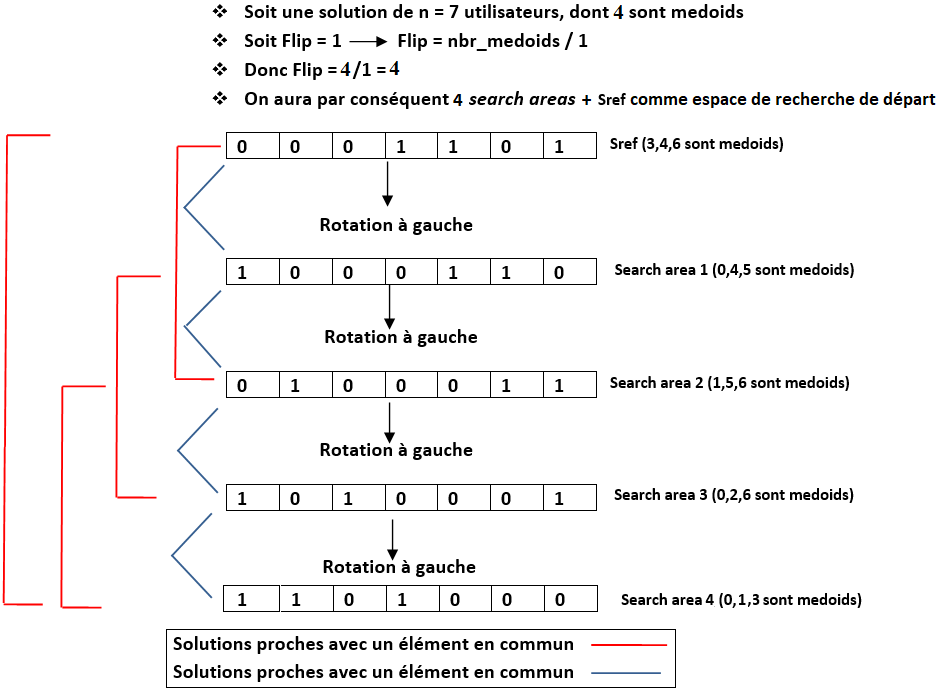
\includegraphics[width=1.1\textwidth]{bsosearch.png}
	\caption{Génération des \textit{search areas} à partir de \textit{Sref}}
	\label{fig:bsosearch}
\end{figure}

\begin{enumerate}[nosep,label=\textbf{\arabic*)}]
	\setcounter{enumi}{4}
	\item \textbf{Fonction fitness}
\end{enumerate}\mbox{}\indent Pour évaluer la qualité du vecteur de solution on a besoin d'évaluer la qualité de la prédiction effectuée à partir du clustering de K-medoids, pour cela nous avons utilisé les métriques RMSE/MAE (à minimiser).
\begin{equation}\label{eq:1}
RMSE = \sqrt{\frac{\sum_{i=1}^{N} (Predicted_{i} - Actual_{i})^{2}  } {N}}  
\end{equation}

\begin{equation}
MAE= \frac {1}{N} \sum_{i=1}^{N} | Predicted_{i} -  Actual_{i}|
\end{equation}

\mbox{}\\Où: 
\begin{itemize}
	\item $Predicted_{i}$: rating prédit pour l'item $i$.
	\item $Actual_{i}$: réel rating  pour l'item $i$.
	\item $N$: nombre d'item total.
\end{itemize}

\begin{enumerate}[nosep,label=\textbf{\arabic*)}]
	\setcounter{enumi}{5}
	\item \textbf{La recherche locale}
\end{enumerate}\mbox{}\indent La recherche locale est effectuée sur chaque vecteur de solution, pour essayer de trouver le nième medoid optimal. 
Une itération de la recherche locale est décrite comme suit:
\begin{enumerate}
	\item Ajouter le nième medoid en changeant la première valeur égale à zéro rencontrée dans le vecteur à un.
	\item Évaluer l'ajout du medoid avec la fonction fiteness, et enregistrer l'évaluation dans une liste nommée \textit{Liste{\_}Eval}.
	\item Défaire l'ajout du nième medoid de l'étape (1).
	\item Refaire les étapes  (1) (2) et (3) pour le reste des valeurs égale à zéro du vecteur solution.
\end{enumerate}
\indent Après avoir terminer le parcours du vecteur solution, on récupère l'indice du medoid qui a donné la meilleure valeur de fonction fitness à partir de \textit{Liste{\_}Eval}, nous affectons à \textit{Sref} la nouvelle solution trouvée dans la recherche locale, et si \textit{nbriterations} n'est pas atteint, alors nous générons des solutions à partir de \textit{Sref} et nous re-effectuant une recherche locale, sinon on sort avec la meilleure solution qui est \textit{Sref}.

\subsubsection*{Calcul de prédiction pour le filtrage avec classification et classification optimisée}Pour la prédiction en se basant sur le vote du cluster auquel appartient chaque utilisateur afin de calculer les ratings des items non encore évalués, et cela en utilisant la formule de la somme pondérée citée précédemment.

\section{Exemple de calcul de prédiction}
Soit la matrice d'usage suivante:
\begin{figure}[H]
	\centering
	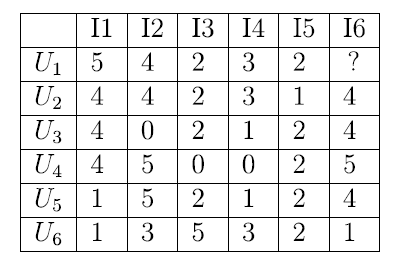
\includegraphics[width=0.40\textwidth]{exemple.PNG}
	\caption{Exemple de matrice d'usage}
	\label{fig:exemple}
\end{figure}
Pour calculer les distances entre les utilisateurs en applique la formule de distance de Pearson suivante:
\begin{equation}
pearson(u,v)= 1 - \frac{\sum_{i \in I} (r_{u,i}-\bar{r}_{u}).(r_{v,i}-\bar{r}_{v})}{\sqrt{\sum_{i \in I} (r_{u,i}-\bar{r}_{u})^{2}.(r_{v,i}-\bar{r}_{v})^{2}}}
\end{equation}
On aura la matrice de distance entre utilisateur comme suit:

\begin{figure}[H]
	\centering
	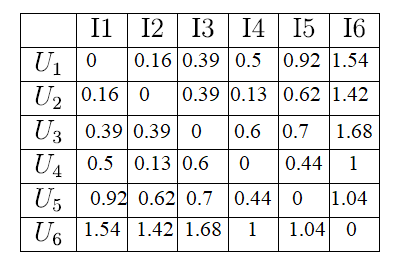
\includegraphics[width=0.45\textwidth]{exemplesim.PNG}
	\caption{Exemple de matrice de distance}
	\label{fig:sim}
\end{figure}

Pour calculer la prédiction de l'utilisateur $U_{1}$ sur l'item $I_{6}$, on effectue tout d'abord un des types de filtrage conçu pour trouver les voisins de chaque utilisateur, on suppose que les voisins de l'utilisateur $U_{1}$ sont comme suit:
 
\begin{figure}[H]
	\centering
	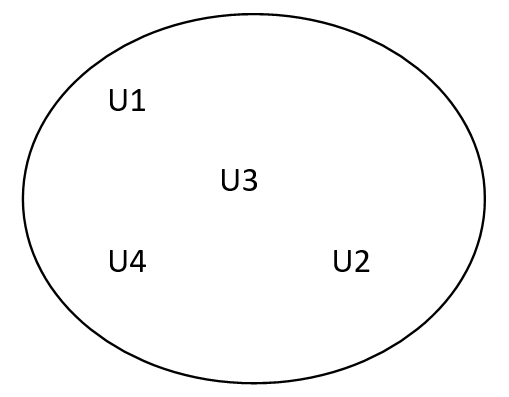
\includegraphics[width=0.35\textwidth]{voisin.PNG}
	\caption{Les voisins de l'utilisateur $U_{1}$}
	\label{fig:voisin}
\end{figure}
En utilisant la formule de prédiction de somme pondérée suivante:
\begin{equation}
pred(u_{i},i_{k})=\bar{r(u_{i})} + \frac{\sum_{u_{j} \in U_{i}} sim(u_{i},u_{j}).(r_{u_{j,ik}}-\bar{r(u_{j})})}{\sum_{u_{j} \in U_{i}} sim(u_{i},u_{j})}
\end{equation}
On aura:
\begin{equation}
pred(u_{1},i_{6})=	3.2 + \frac{0.16 * (4-3) + 0.39 * (4-2.6) + 0.5 * ( 5-4)}{ 0.16 + 0.39 + 0.5}= 4.38
\end{equation}
\section {Ingénierie du système}
Nous présentons le diagramme de cas d'utilisation qui modélise les différentes fonctionnalités de notre système de recommandation.
\begin{figure}[H]
	
	\centering
	\hspace*{-0.85in}
	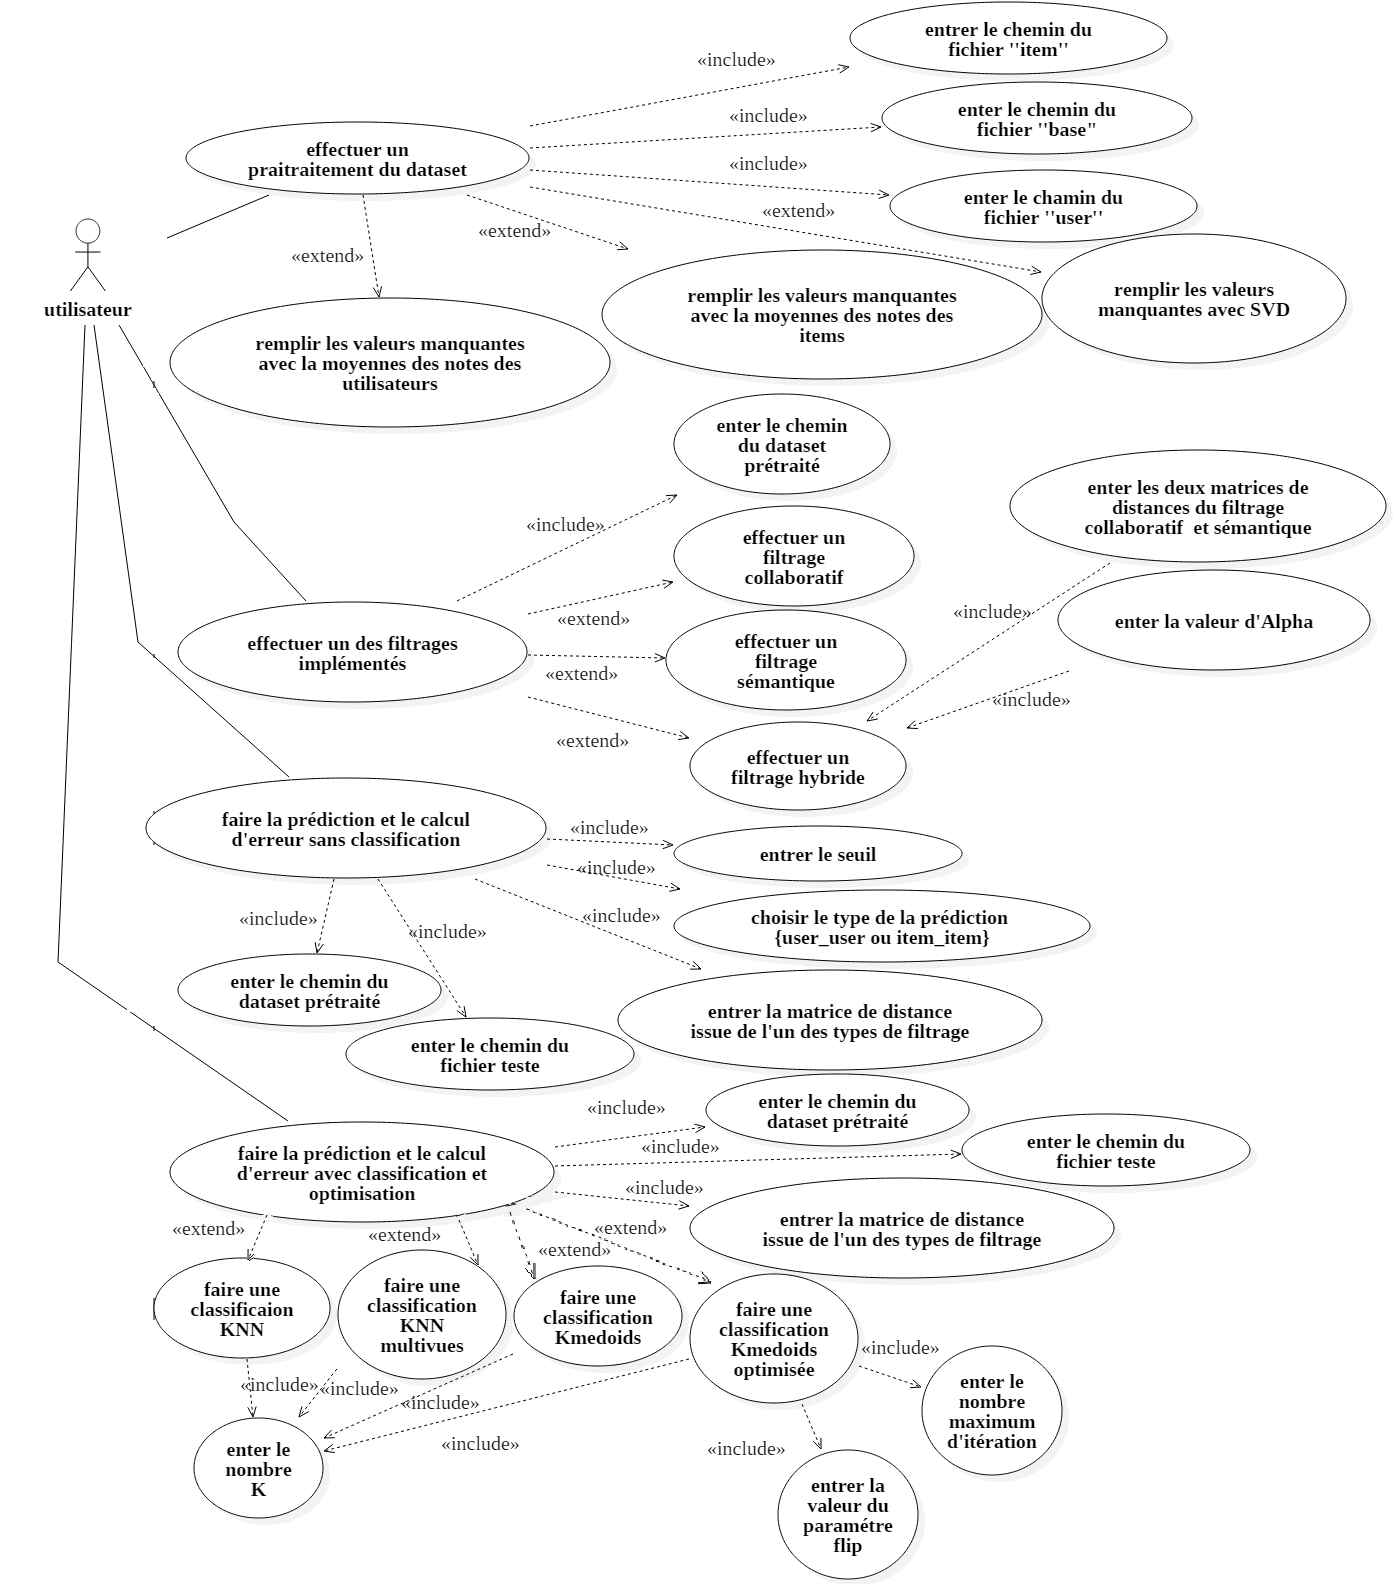
\includegraphics[width=1.2\textwidth]{shemaglobalesys.PNG}
	
	\caption{Diagramme de cas d'utilisation de notre système de recommandation}
	
	\label{fig:shemaglobalesys}
	
\end{figure}
\section {Conclusion}
Dans ce chapitre nous avons présenté en détail notre approche de recommandation qui utilise trois types de filtrage: Collaboratif, sémantique et hybride (combinant ces deux algorithmes selon différentes méthodes). Dans un second lieu, nous avons appliqué deux techniques de classification, supervisée (L'algorithme KNN a été utilisé) et non supervisée (l'algorithme K-medoids a été utilisé). Une hybridation basé sur ces algorithmes a été considéré, dont l'hybridation multivues avec KNN. Finalement, afin d'améliorer la qualité de la classification, nous avons appliqué une optimisation en utilisant la métaheuristique BSO (algorithme K-medoids-BSO). 
Dans le chapitre suivant nous allons évaluer notre système de recommandation et présenter l'interface réalisée qui permet aux utilisateurs de tester notre système et de visualiser les résultats obtenus.

\chapter{Implémentation et expérimentation }
\thispagestyle{empty}
\newpage
\section{Introduction}
Dans le chapitre précédent, nous avons proposé une approche de recommandation incluant plusieurs algorithmes basés sur des techniques différentes (hybridation, clustering, clustering optimisé et clustering multivues). 
Dans ce chapitre, nous présenterons en détail l'implémentation et l'expérimentation de notre système de recommandation.
Ce chapitre est structuré comme suit:
\begin{itemize}
	\item L'environnement de travail (langage, outils et bibliothèques utilisés),
	\item L’application réalisée, (son fonctionnement et mode d’emploi),
	\item L'analyse des performances de l’approche développée et la comparaison de nos résultat avec ceux d’autres techniques déjà existantes.
\end{itemize}

\section{Environnement de travail}
Nous allons présenter dans cette partie les outils que nous avons utilisé pour réaliser notre système de recommandation.
\subsection{Langage de programmation \textit{Python}}
Créé originellement par le programmeur Guido van Rossum autour de 1990, \textit{Python} est un langage de programmation objet interprété de haut niveau avec une sémantique dynamique. Ses structures de données intégrées de haut niveau, combinées à un typage et liaison dynamique, le rendent très attrayant pour le développement rapide d'applications, ainsi que pour son utilisation en tant que langage de script ou de collage pour connecter des composants existants\cite{ref39}.


\myparagraph{Caractéristiques du langage et avantages}
\begin{itemize}
	\item La syntaxe simple et facile à apprendre de Python met l'accent sur la lisibilité et réduit donc le coût de la maintenance du programme. 
	\item Python prend en charge les modules et les packages, ce qui encourage la modularité du programme et la réutilisation du code. 
	\item L'interpréteur Python et la vaste bibliothèque standard sont disponibles gratuitement sous forme binaire ou source pour toutes les principales plates-formes et peuvent être distribués librement.
\end{itemize}

\subsection{Outils et logiciels}
\myparagraph{Système d’exploitation (Linux)}Linux est un noyau monolithique à code source ouvert. Le noyau Linux a été développé à l'origine par Linus Torvalds, qui l'a annoncé dans le groupe de discussion comp.os.minix le 25 août 1991. Depuis lors, il a été porté sur des architectures informatiques comprenant x86-64, x86, ARM, RISC et DEC Alpha. Les développeurs ont accès à tout le code source de Linux et sont autorisés, dans les conditions de la licence, à le modifier et à le distribuer \cite{ref40}.

\myparagraph{L’environnement de développement (Visual Studio
Code)}
Visual Studio Code est un éditeur de code source gratuit et libre de droit, disponible pour Windows, macOS et Linux. Il est livré avec un support intégré pour JavaScript, TypeScript et Node.js et dispose d'un écosystème riche en extensions pour d'autres langages (tels que C ++, C\#, Java, Python, PHP, Go) \cite{ref41}.

\section{Présentation de notre système de recommandation}
\subsection{Description générale}
Le système que nous avons développé permettra de lancer les différents
algorithmes implémentés et de visualiser en détails les performances et les résultats de chaque technique stockés dans des fichiers \textit{.csv}.

Il sera également possible de choisir le dataset (jeux de données) à utiliser. Toutes les techniques implémentées sont généralisées pour traiter n’importe quel dataset possédant la structure montrée dans la figure \ref{fig:shemfi}.
La modularité du code source de l’application permettra facilement d’apporter des mises à jours aux algorithmes afin d'ajouter d'autre techniques.
\begin{figure}[H]
	\centering
	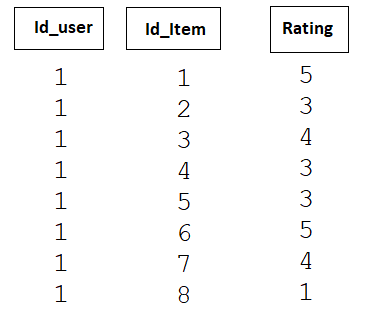
\includegraphics[width=0.5\textwidth]{shemfi.PNG}
	\caption{Exemple de structuration d'un fichier exploitable dans notre système de recommandation}
	\label{fig:shemfi}
\end{figure}



\subsection{Illustration des fonctionnalités développées}
L'interface de l'application est composée de 4 onglets, qui sont:
\begin{itemize}
	\item\textit{Data preprocessing}: le prétaitement des données d'un dataset est une étape essentielle avant son utilisation, dans notre cas il existe énormément de valeurs manquantes de rating  car les users ne notent pas tous les items existants et par conséquent la prédiction effectuée ne sera pas précise.
	Pour effectuer un prétraitement du dataset, il faut passer en entrée trois fichiers, qui sont: 
	\begin{itemize}
		\item Fichier \textit{u.item}: contient les identificateurs des items.
		\item Fichier \textit{u.user}: contient les identificateurs des utilisateurs.
		\item Fichier \textit{u.base}: contient les évaluations faites par les utilisateurs sur les items.
	\end{itemize}
	Le traitement des valeurs manquantes s'effectue avec l'une des options suivantes:
	\begin{itemize}
		\item Moyenne de rating des utilisateurs: on remplace les valeurs manquantes en effectuant la moyenne des évaluations des utilisateurs, pour voir en général la note que ces derniers attribuent aux items.
		
		\item Moyenne de rating des items: les valeurs manquantes d'un item sont remplacées par la moyenne des évaluations qu'il lui sont attribuées.
		
		\item SVD: nous utilisons la technique SVD expliqué dans le chapitre 3, afin d'effectuer une décomposition de la matrice d'usage du dataset pour extraire les caractéristiques cachées des items et des utilisateurs et ainsi les faire correspondre selon leurs caractéristiques, et remplacer les valeurs manquantes des ratings.
		
		On note qu'on peut laisser le fichier tel quel sans prétraitement.
	\end{itemize}

Quand le prétraitement des données est effectué, le résultat est sauvegardé dans un fichier pour une exploitation ultérieure.


\begin{figure}[H]
	\centering
	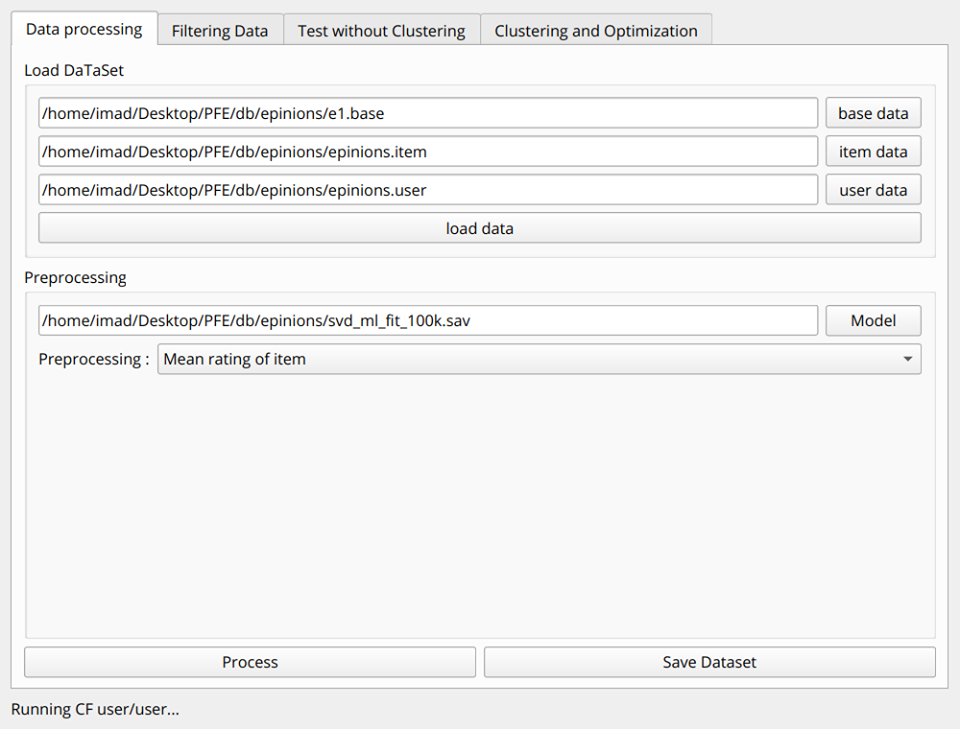
\includegraphics[width=\textwidth]{datapre.PNG}
	\caption{Capture d'écran de l'onglet \textit{Data preprocessing}}
	\label{fig:datapre}
\end{figure}

	\item \textit{Filtering data}: dans cet onglet on effectue l'un des filtrage conçu (FC, FSem, hybride), le fichier prétraité dans l'étape précédent est importé puis le calcul des distances entre les utilisateurs s'effectue avec les formules de similarité des filtrage et le résultat est sauvegardé dans un fichier (stockage de la matrice des distances dans un fichier).
	
	\begin{figure}[H]
		\centering
		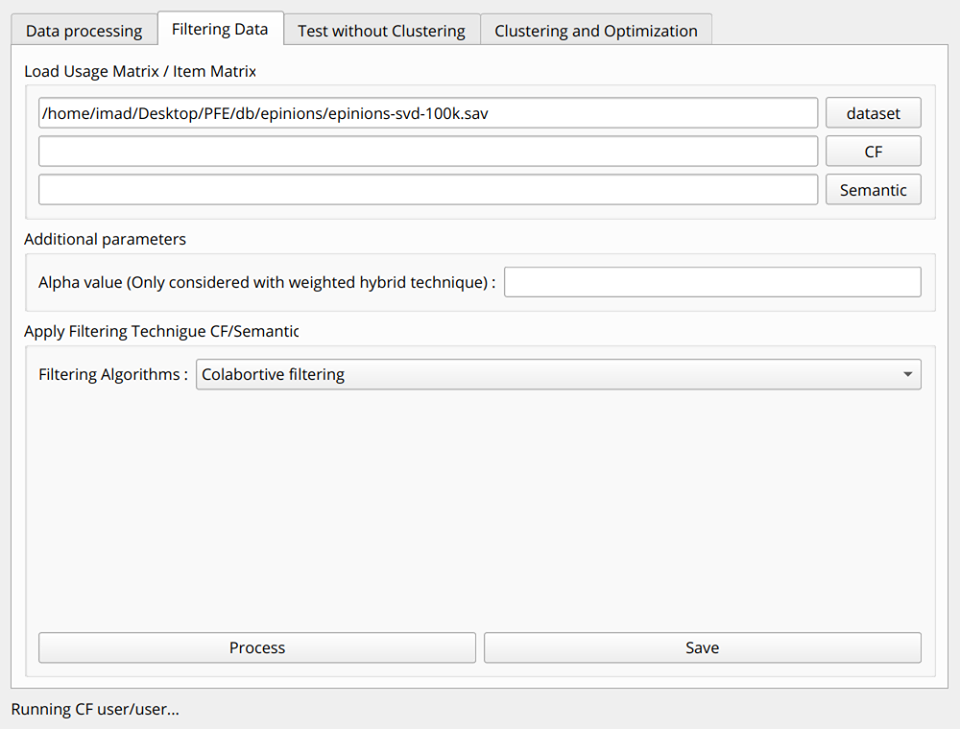
\includegraphics[width=\textwidth]{filter.PNG}
		\caption{Capture d'écran de l'onglet \textit{Filtering data}}
		\label{fig:filter}
	\end{figure}
	\item \textit{Test without classification}: comme expliqué dans le chapitre précédent, après avoir obtenu la matrice de distances qui est issue de l'un des types de filtrage on peut effectuer les prédictions des évaluations des items en utilisant un seuil qui permet la sélection des voisins des utilisateurs (ou les items pour le cas FC item-item).
	On commence par introduire le fichier prétraité d'un dataset, car il contient les évaluations des items donnés par les users, puis la matrice de distance du dataset pour la sélection des voisins des users. Le type de la matrice de distance qu'on introduit dépend des cas suivant:
	\begin{itemize}
		\item Si FC item-item alors introduire matrice de distance item-item calculée avec formule de Pearson.
		\item Si FC user-user alors introduire matrice de distance user-user calculée avec formule de Pearson.
		\item Si FSem alors introduire matrice de distance user-user calculée avec formule distance d'interet.
		\item Si filtrage hybride alors introduire matrice de distance hybride calculée avec formule Pearson et distance d'intérêt.
	\end{itemize}
	
	Après avoir importer les fichier du dataset prétraité et sa matrice de distance, on importe le fichier test qui contient les ratings des items pour effectuer les prédictions et vérifier la qualité de cette dernière avec les métriques RMSE et MAE vus dans le chapitre précédent et les affichées dans l'interface.
	
	\begin{figure}[H]
		\centering
		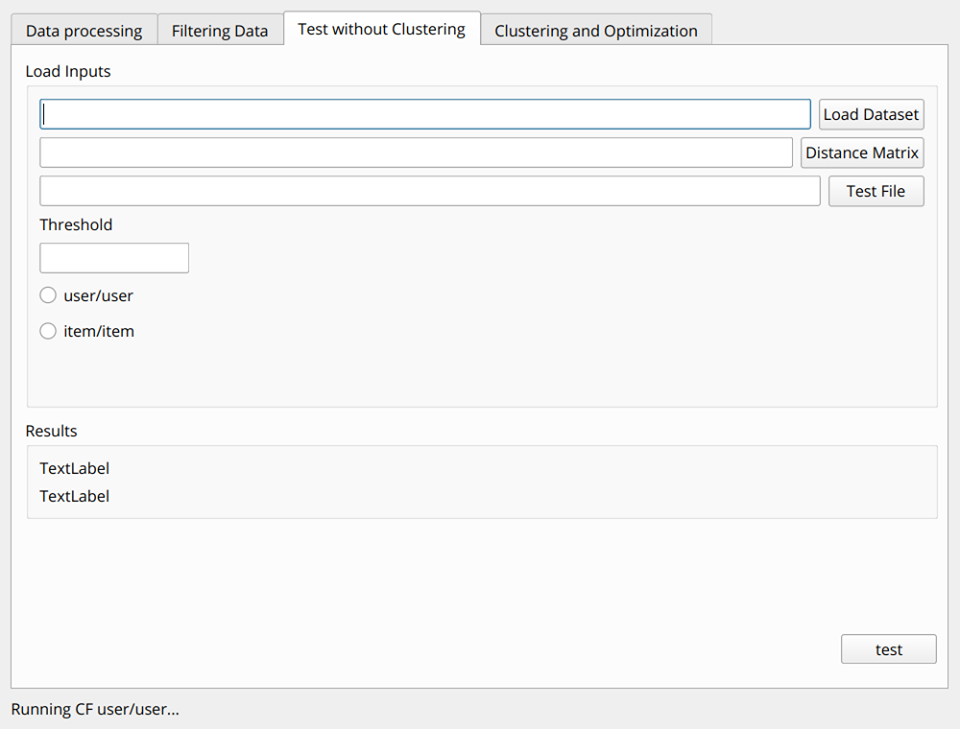
\includegraphics[width=\textwidth]{sansclus.PNG}
		\caption{Capture d'écran de l'onglet \textit{Test without classification}}
		\label{fig:sansclus}
	\end{figure}
	\item \textit{Classification and optimisation}: pour faire un filtrage avec classification ou classification optimisée,  les mêmes étapes de l'onglet \textit{test without clustering} sont reeffectuées sauf qu'au lieu d'introduire un seuil de sélection de voisins, on utilise un algorithme de classification sur la matrice de distances des users (respectivement des items pour le FC item-item avec classification).
	Après avoir introduit les fichiers contenant le dataset, la matrice de distances et les items de test, on entre les paramétrés selon la technique de classification voulue:
	
	\begin{itemize}
		\item K-medoids: le nombre K de cluster est requis pour lancer une classification avec K-medoids des utilisateurs.
		\item K-medoids optimisé: le nombre K de cluster à former et \textit{max iterations} qui est le nombre maximum d'itération à effectuer pour trouver une solution optimisée.
		\item K-NN: le nombre K de voisins à considérer pour les prédictions des ratings de chaque utilisateur.
		\item K-NN multiview: (le même paramètre que K-NN est requis pour exécuter K-NN multiview).
	\end{itemize} 
	Les résultats des évaluations des prédictions sera affiché après exécution des algorithmes dans l'interface est qui sont: RMSE, MAE, rappel, précision. 

\begin{figure}[H]
	\centering
	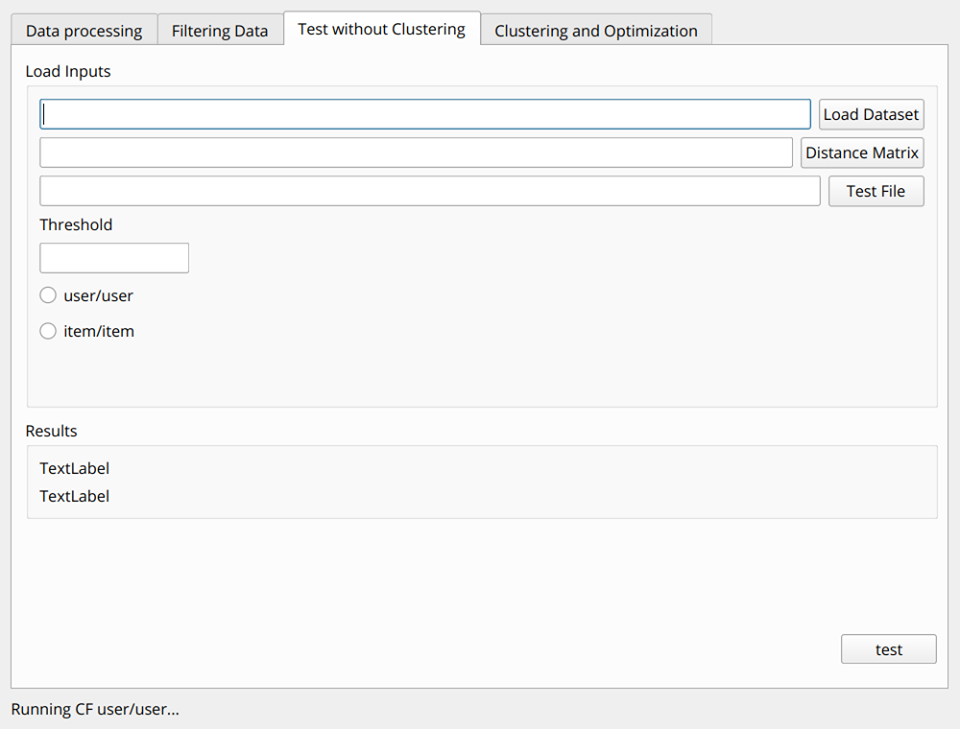
\includegraphics[width=\textwidth]{sansclus.PNG}
	\caption{Capture d'écran de l'onglet \textit{Classification and optimisation}}
	\label{fig:clasificationonglet}
\end{figure}


\end{itemize}



\section{Expérimentation}
\subsection{Dataset}
\begin{enumerate}[nosep,label=\textbf{\arabic*)}]
	%%\setcounter{enumi}{2}
	\item \textbf{Présentation de \textit{MovieLens}}
\end{enumerate}\mbox{} \indent GroupLens Research (un laboratoire de recherche de l’université du Minnesota) a mis à disposition un ensemble de données d’évaluation à partir du site Web MovieLens collectés sur différentes périodes.
On retrouve des jeux de données allant de 100 000 évaluations jusqu'à 20 millions, ce dernier est plus destinées à la recherche ou de grand moyens matériels sont souvent nécessaires.
Étant limité par le temps et par la puissance de calcul de nos machines, nous
opterons donc dans un premier temps pour des dataset de 100 000 évaluations afin d’effectuer nos tests.

\myparagraph{Architecture du dataset}Le dataset \textit{100K} de \textit{MovieLens} se présente sous la structure suivante :
\begin{itemize}
	\item Un fichier \textit{u.data}: de 100 000 lignes, contenant l’ensemble des évaluations (l’id de l’utilisateur, l’id de l’item, l’évaluation (de 1 à 5), la date d’évaluation).
	\item  Un fichier \textit{u.genre}: ou on peut retrouver les différent catégories des films présents sur la plate-forme.
	\item  Un fichier \textit{u.item}: ou sont indiqués tous les films avec l’ensemble des informations qui leurs sont relatives : date de sortie, genre etc ...
	\item Un fichier \textit{u.occupation}: indiquant les différentes professions des utilisateurs.
	\item  Un fichier \textit{u.user}: contenant les informations relatives à chaque utilisateur: age, sexe, profession etc ...
	\item  Un fichier \textit{u.base}: contient 80\%  des données \textit{u.data}, ce fichier est utilisé pour effectuer l'apprentissage (classification et construction de modèle).
	\item  Un fichier \textit{u.test}: contient 20\%  des données \textit{u.data}, ce fichier est utilisé pour effectuer les testes (prédiction et calcule d'erreur).
\end{itemize}
\subsubsection*{Exploitation du dataset}
Le processus de test et d’évaluation d’un algorithme nécessite deux ensembles de données : un ensemble d’apprentissage et un ensemble de test.
En effet, l’ensemble de données du fichier \textit{u.data} contient en tout 100 000 évaluations, nous prendrons donc \textit{u.base} qui contient 80 000 évaluations pour l’apprentissage et \textit{u.test} qui contient 20 000 évaluations pour la prédiction et le calcul des métriques.

\begin{enumerate}[nosep,label=\textbf{\arabic*)}]
	\setcounter{enumi}{1}
	\item \textbf{Présentation de \textit{RED}}
\end{enumerate}\mbox{} \indent Epinions.com était un un site général d'évaluation des consommateurs créé en 1999. Epinions a été acquis par Shopping.com (connu sous le nom de DealTime au moment de l'acquisition) en 2003, qui a ensuite été acquis par eBay en 2005. Chez Epinions, les visiteurs pouvaient lire nouvelles et anciennes critiques sur une variété d’articles pour les aider à effectuer leurs achats. Le 25 mars 2014, toutes les fonctionnalités de la communauté, ainsi que les fonctionnalités de soumission et de modification des avis, ont été désactivées. Par la suite, en mai 2018, le site a été complètement fermé et les URL du domaine epinions.com sont redirigées vers Shopping.com.

RED: (\textit{Rich Epinions Dataset for Recommender Systems}) est un jeu de données extrait d'Epinions et enrichi. Il contient des critiques d'utilisateurs sur les éléments, les valeurs de confiance entre les utilisateurs, la catégorie d'éléments, la hiérarchie des catégories et l'expertise des utilisateurs sur les catégories. Cet ensemble de données peut être utilisé pour évaluer divers systèmes de recommandation.

\myparagraph{Architecture du dataset}
Le dataset est une base de données relationnelle avec les tables suivantes:
\begin{itemize}
	\item Utilisateur: nom (pseudo et URL du profil), location, rang (peut être nul) et les visites de profil.
	\item Item: nom, catégorie et URL du profil.
	\item  Catégorie: nom, catégorie parent, url de description, lignage (chemin dans l'arborescence des catégories) et profondeur (dans l'arborescence des catégories).
	\item Critique: une critique associe un utilisateur à un élément, elle contient la note, entre 1 et 5, la note de la revue (moyenne de toutes les notes associées à cette critique) et la date de révision.
	\item Expertise: les utilisateurs experts dans une catégorie apparaissent ici avec l'expertise (responsable de la catégorie, examinateur principal, conseiller) associée à la catégorie considérée.
	\item Trust: Web de confiance, c’est-à-dire une valeur de confiance (-1 ou 1) d’un utilisateur à un autre, seules les valeurs de confiance positives apparaissent dans le jeu de données.
	\item Similarité: la similarité entre tous les couples d'utilisateurs avec la corrélation de coefficient de Pearson. 
\end{itemize}

\begin{figure}[H]
	\centering
	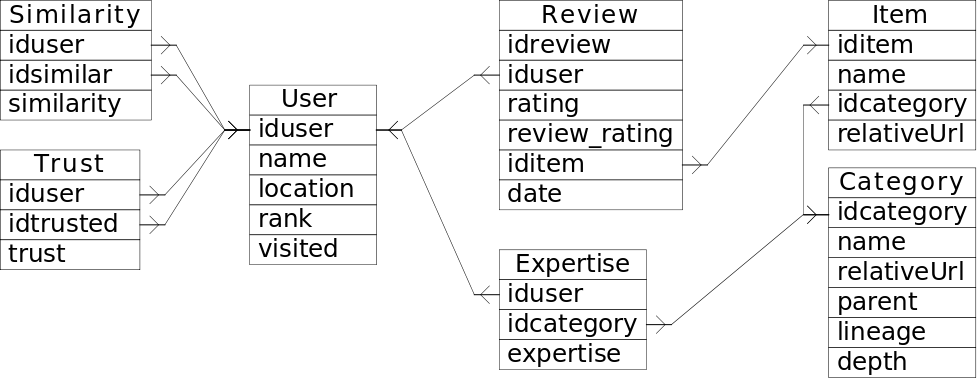
\includegraphics[width=\textwidth]{shemata.PNG}
	\caption{Architecture de la base de données RED}
	\label{fig:shemta}
\end{figure}
\subsubsection*{Exploitation du dataset}
Nous avons pris un échantillon du dataset RED, qui est formé de 100K ratings de 149 utilisateurs sur 5000 items, et nous avons divisé cette échantillon en deux ensemble de données, un ensemble d'apprentissage environ 80\% de l'échantillon et un ensemble de 20\% pour les testes. 
\subsection{Métriques d'évaluation}
Nous nous baserons sur deux métriques afin d’évaluer notre travail : MAE et RMSE cité dans le chapitre précédant (voir formule \ref{eq:1}), qui sont des métriques permettant de calculer la différence
entre deux variables continues. En effet, ces deux métriques restent les plus utilisées dans le domaine et les plus pertinentes quant à évaluer la qualité d’un système de recommandation.

\subsection{Résultats des évaluations}
Dans cette partie, nous réaliserons un ensemble de tests portant sur les performances de notre approche et nous comparerons nos résultats avec les résultats des approches existantes. 
\textbf{A) Évaluations avec MovieLens-100K}
\begin{enumerate}[nosep,label=\textbf{\arabic*)}]
	%%  \setcounter{enumi}{4}
	\item \textbf{Filtrage collaboratif}
\end{enumerate}
\subsubsection*{FC sans classification}
Dans cette phase d’expérimentations, nous allons évaluer la qualité de la recommandation lorsque celle-ci est basée sur un filtrage collaboratif standard (user-user, item-item, SVD). Nous ferons des expérimentations par rapport à la corrélation de Pearson, étant donné que celle-ci reste l’une des plus connues et des plus utilisées.
Nous avons évalué les algorithmes suivants:
\begin{itemize}
	\item  FC item-item avec un praitrétement la moyenne des évaluations des utilisateur 
	(FC-item-item-UA).
	\item  FC item-item avec un praitrétement la moyenne des évaluations des items (FC-item-item-IA).
	\item  FC item-item avec un praitrétement la méthode SVD (FC-item-item-SVD).
	\item FC item-item sans prétraitement (FC-item-item).
	\item  FC user-user avec un praitrétement la moyenne des évaluations des utilisateur (FC-user-user-UA).
	\item  FC user-user avec un praitrétement la moyenne des évaluations des items (FC-user-user-IA).
	\item  FC user-user avec un praitrétement la méthode SVD (FC-user-user-SVD).
	\item FC user-user sans prétraitement (FC-user-user).	
\end{itemize}
\begin{figure}[H]
	\centering
	\includegraphics[width=\textwidth]{MAEFC.PNG}
	\caption{Évaluation MAE du FC standard en fonction du seuil}
	\label{fig:FCMAE}
\end{figure}

\begin{figure}[H]
		\centering
	\includegraphics[width=\textwidth]{RMSEFC.PNG}
	\caption{Évaluation RMSE du FC standard en fonction du seuil}
	\label{fig:FCRMSE}
\end{figure}

\begin{center}\label{tab1}
	\begin{tabularx}{\textwidth}{|p{3.7cm}|l|l|l||p{3.65cm}|l|l|l|}
		\hline
		threshold & 0.258 & 0.345 & 0.301 & threshold & 0.073 & 0.109 & 0.256 \\ \hline
		MAE  (FC-item-UA) & 0.796 & 0.797 & 0.798 & MAE  (FC-user-IA) & 0.798 & 0.799 & 0.8 \\ \hline
		RMSE (FC-item-UA) & 1.067 & 1.067 & 1.068 & RMSE (FC-user-IA) & 1.069 & 1.07 & 1.07 \\ \hline\hline
		threshold & 0.284 & 0.227 & 0.17 & threshold & 0.4 & 0.6 & 0.5 \\ \hline
		MAE  (FC-user-SVD) & \textbf{0.73} & 0.736 & 0.75 & MAE  (FC-item-IA) & 0.775 & 0.78 & 0.782 \\ \hline
		RMSE (FC-user-SVD) & \textbf{1.001} & 1.007 & 1.023 & RMSE (FC-item-IA) & 1.064 & 1.066 & 1.07 \\ \hline\hline
		threshold & 0.454 & 0.606 & 0.53 & threshold & 0.151 & 0.227 & 0.303 \\ \hline
		MAE  (FC-user-ua) & 0.761 & 0.78 & 0.781 & MAE  (FC-user-user) & 0.795 & 0.81 & 1.022 \\ \hline
		RMSE (FC-user-ua) & 1.047 & 1.066 & 1.066 & RMSE (FC-user-user) & 1.079 & 1.111 & 1.492 \\ \hline\hline
		threshold & 0 & 0.105 & 0.158 & threshold & 0 & 0.1 & 0.2 \\ \hline
		MAE  (FC-item-SVD) & 0.923 & 0.93 & 0.94 & MAE  (FC-item-item) & 0.804 & 0.808 & 0.829 \\ \hline
		RMSE (FC-item-SVD) & 1.197 & 1.207 & 1.217 & RMSE (FC-item) & 1.076 & 1.085 & 1.133 \\ \hline
	\end{tabularx}	
	\captionof{table}{Récapitulatif des trois meilleurs résultats (MAE et RMSE) pour chaque FC sans classification} 
\end{center}
\subsubsection*{Discussion des résultats}
En analysant les deux figures ci-dessus, il est clair qu’au delà d’un certain seuil, environ 0.5, la qualité de la prédiction stagne pour les différent types de FC.

On remarque que lorsque le dataset n'est pas prétraité les résultats sont de qualité médiocre, ce qui confirme l'importance du prétraitement du dataset, les meilleures valeurs de MAE et RMSE sont au alentour de respectivement 0.80 et 1.2 dans le cas de FC user-user et FC item-item.

Les deux filtrages collaboratif user-user avec comme prétraitement la moyennes des items (FC-user-user-IA) et FC item-item avec  prétraitement la moyenne des users (FC-item-item-UA), donnent des résultat presque similaire environ  0.79 pour le meilleur MAE et 1.06 pour RMSE.
 
L'utilisation de la technique de SVD pour le prétraitement et l'application d'un FC item-item  par la suite (FC-item-item-SVD), donne de très mauvais résultats, donc cette technique est à exclure pour la suite des évaluations avec classification.

Le filtrage qui a donné les meilleures évaluations est FC user-user (FC-user-user-SVD) avec comme prétraitment SVD, et la meilleure valeur de MAE est égale à 0.73 et RMSE égale à 1.001, pour un seuil de 0.284, donc nous allons opté pour ce filtrage dans la suite des évaluations.

\subsubsection*{FC Avec classification}
Pour cette approche, nous ferons varier la valeur de k dans les algorithmes de FC avec classification, et essayer de déduire laquelle de ses valeurs nous permettra d’atteindre les meilleurs résultats.
Nous avons évalué les algorithmes suivants:
\begin{itemize}
	\item  FC user-user basé K-medoids (FC-user-user-Kmedoids).
	\item  FC user-user basé K-medoids et BSO (FC-user-user-Kmedoids-BSO).
	\item  FC user-user basé K-KNN (FC-user-user-KNN).
\end{itemize}

\begin{figure}[H]
		\centering
	\includegraphics[width=\textwidth]{MAEclassFC.PNG}
	\caption{Évaluation MAE du FC avec classification en fonction du seuil}
	\label{fig:MAEclassFC}
\end{figure}


\begin{figure}[H]
		\centering
	\includegraphics[width=\textwidth]{RMSEclassFC.PNG}
	\caption{Évaluation RMSE du FC avec classification en fonction du seuil}
	\label{fig:RMSEclassFC}
\end{figure}
\begin{table}[H]
	\centering
	\begin{tabular}{|l|l|l|l|}
		\hline
		threshold & 0.284 & 0.227 & 0.17 \\ \hline
		MAE  (FC-user-SVD) & \textbf{0.73} & 0.736 & 0.75\\ \hline
		RMSE (FC-user-SVD) & \textbf{1.001} & 1.007 & 1.023 \\\hline \hline
		K & 10 & 15 & 45 \\ \hline
		MAE(FC-kmedoids) & 0.733 & 0.732 & 0.734 \\ \hline
		RMSE(FC-svd-kmedoids) & 1.004 & 1.003 & 1.007 \\ \hline\hline
		K & 25 & 15 & 20 \\ \hline
		MAE(FC-kmedoids-bso) & \textbf{0.728} & 0.729 & 0.73 \\ \hline
		RMSE(FC-kmedoids-bso) & \textbf{1.001} & 1.001 & 1.001 \\ \hline\hline
		K & 50 & 40 & 30 \\ \hline
		MAE(FC-KNN) & 0.73 & 0.731 & 0.732 \\ \hline
		RMSE(FC-KNN) & 1.001 & 1.001 & 1.002 \\ \hline
	\end{tabular}
\captionof{table}{Récapitulatif des trois meilleurs résultats (MAE et RMSE) pour l'algorithme de FC avec classification}
\end{table}
\subsubsection*{Discussion des résultats}
Comme nous pouvons le constater sur les figures \ref{fig:MAEclassFC} et \ref{fig:RMSEclassFC} ci-dessus, la qualité de la prédiction évolue selon le nombre de voisins choisis. En prenant plus de 85 voisins la qualité semble diminuer pour les trois algorithme.

L'ajout du clustering au FC avec comme prétraiement SVD ne semble pas améliorer les résultats car la meilleure valeur de MAE obtenu est 0.733 pour FC basé Kmedoids alors que FC avec SVD elle était égale à 0.73, on suppose que le choix aléatoire des medoids est la cause de la non amélioration des évaluations, de ce fait une optimisation du choix des medoids est nécessaire pour voir l'apport de classification.

Nous pouvons constater que le FC basé Kmedoids-BSO améliore les résultats de FC basé K-medoids et FC standard, avec MAE égale à 0.728, ce qui confirme l'apport de l'optimisation sur le clustering et donc on peut dire que le clustering peut améliorer les résultats d'un FC standard si le jeu de teste est d'un volume plus important.

En ce qui concerne le FC basé K-NN, il n'améliore pas la qualité des évaluations du FC standard mais donne de résultats plus au moins stable avec MAE ne dépassant pas les 0.74 et RMSE les 1.005.

%%%%%%%%%%%%%%%%%%%%%%%FILTRAGE SEMANTIQUE%%%%%%%%%%%%%%%%%%%%%%%%%
\mbox{}\\
\begin{enumerate}[nosep,label=\textbf{\arabic*)}]
	 \setcounter{enumi}{1}
	\item \textbf{Filtrage sémantique standard}
	\end{enumerate}\mbox{} \indent Dans cette phase d’expérimentations, nous allons évaluer la qualité de la recommandation lorsque celle-ci est basée sur un filtrage sémantique. Nous ferons des expérimentations en utilisant la formule de distance d'intérêt entre utilisateur, et la distance de Jaccard entre les items car le dataset MovieLense ne possède pas une représentation sous forme d'ontologie des items.
Le prétraitement des valeurs manquantes est effectué avec la méthode SVD.

\subsubsection*{FSem sans classification}
Nous avons évalué l'algorithme FSem user-user.

\begin{figure}[H]
		\centering
	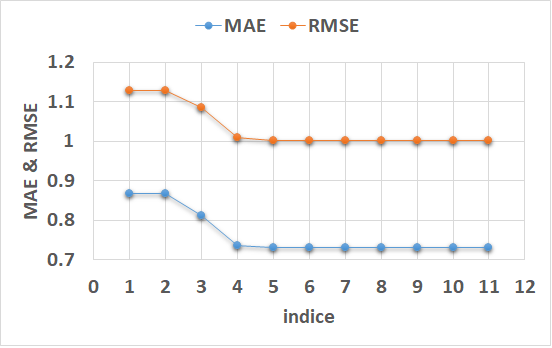
\includegraphics[width=0.8\textwidth]{semsvd.PNG}
	\caption{Évaluation MAE et RMSE du FSem en fonction du seuil de similarité}
	\label{fig:MAEsem}
\end{figure}

Afin de ne pas encombré le graphe ci-dessus (\ref{fig:MAEsem}) nous avons indexé les onze valeurs des seuils du FSem et nous les avons mis dans le tableau suivant:

\begin{table}[H]
	\centering
	\begin{tabular}{|l|l|}
		\hline
		indice & threshold \\ \hline
		1 & 0.6666666666666 564 \\ \hline
		2 & 0.6666666666666 592\\ \hline
		3 & 0.6666666666666 62 \\ \hline
		4 & 0.6666666666666 647 \\ \hline
		5 & 0.6666666666666 675 \\ \hline
		6 & 0.6666666666666 703 \\ \hline
		7 & 0.6666666666666 731 \\ \hline
		8 & 0.6666666666666 758 \\ \hline
		9 & 0.6666666666666 786 \\ \hline
	   10 & 0.6666666666666 814 \\ \hline
	   11 & 0.6666666666666 842 \\ \hline
	\end{tabular}
\captionof{table}{Les valeurs de seuils correspondant aux indices du graphes \ref{fig:MAEsem}}
\end{table}

\begin{center}
	\begin{tabularx}{\textwidth}{|p{5.1cm}|p{3.2cm}|p{3.2cm}|p{3.3cm}|}
		\hline
		indice& 5 & 6 & 9 \\ \hline
		MAE  (FSem-user-user) & \textbf{0.7297} & 0.7306 & 0.7303 \\ \hline
		RMSE (FSem-user-user) & \textbf{1.0012} & 1.0022 & 1.0020\\ \hline
	\end{tabularx}
\captionof{table}{Récapitulatif des trois meilleurs résultats (MAE et RMSE) pour l'algorithme de FSem sans classification}
\end{center}

\subsubsection*{Discussion des résultats}
En analysant la figure \ref{fig:MAEsem} ci-dessus, il est clair qu’au delà d’un certain seuil, plus précisément le seuil possédant l'indice 6, la qualité de la prédiction stagne au alentour de 0.73 pour MAE et 1.002 pour RMSE.

On constate que la meilleure valeur du seuil à choisir dans le FSem standard est le seuil possédant l'indice 5, qui à donné MAE égale à 0.729 et RMSE égale à 1.001.

\subsubsection*{FSem avec classification}
Pour cette approche, nous ferons varier la valeur de K dans les algorithme de FSem avec classification, et essayer de déduire laquelle de ses valeurs nous permettra d’atteindre les meilleurs résultats.
Nous avons évalué les algorithmes suivant:
\begin{itemize}
	\item  FSem user-user basé K-medoids (FSem-user-user-Kmedoids).
	\item  FSem user-user basé K-medoids et BSO (FSem-user-user-Kmedoids-BSO).
	\item  FSem user-user basé K-NN (FSem-user-user-KNN).
\end{itemize}
\begin{figure}[H]
	\centering
	\includegraphics[width=0.9\textwidth]{semMAEclass.PNG}
	\caption{Évaluation MAE avec les algorithmes de FSem basés classification}
	\label{fig:semMAEclass}
\end{figure}

\begin{figure}[H]
	\centering
	\includegraphics[width=0.9\textwidth]{RMSEclasssem.PNG}
	\caption{Évaluation RMSE avec les algorithmes de FSem basés classification}
	\label{fig:RMSEclasssem}
\end{figure}

\begin{center}\label{tab2}
	\begin{tabularx}{\textwidth}{|p{5.1cm}|p{3.2cm}|p{3.2cm}|p{3.3cm}|}
	\hline
	indice & 5 & 6 & 9 \\ \hline
	MAE  (FSem-user-user) & \textbf{0.7297} & 0.7306 & 0.7303 \\ \hline
	RMSE (FSem-user-user) & 1.0012 & 1.0022 & 1.0020\\ \hline	
	\hline
	k & 10 & 15 & 20 \\ \hline
	MAE  (FSem-user-user-kmedoids-bso) & 0.728 & 0.7292 & 0.7293 \\ \hline
	RMSE (FSem-user-user-kmedoids-bso) & 1.002 & 1.0012 & 1.005 \\ \hline\hline
	k & 55 & 65 & 60 \\ \hline
	MAE  (Fsem-user-user-KNN) & \textbf{0.7297} & 0.7299 & 0.7301 \\ \hline
	RMSE (Fsem-user-user-KNN) & \textbf{1.0007} & 1.0006 & 1.0003 \\ \hline\hline
	k & 15 & 25 & 10 \\ \hline
	MAE  (FSem-user-user-kmedoid) & 0.7301 & 0.7307 & 0.7309 \\ \hline
	RMSE (FSem-user-user-kmedoid) & 1.0012 & 1.0027 & 1.002 \\ \hline
\end{tabularx}
\captionof{table}{Récapitulatif des trois meilleurs résultats (MAE et RMSE) pour l'algorithme de FSem avec classification}
\end{center}

\subsubsection*{Discussion des résultats}
Comme nous pouvons le constater sur les figures \ref{fig:semMAEclass} et \ref{fig:RMSEclasssem} ci-dessus, la qualité de la prédiction évolue selon le nombre de voisins choisis. En prenant plus de 85 voisins la qualité semble diminuer pour les trois algorithme.

L'ajout du clustering au FSem avec comme prétraiement SVD ne semble pas améliorer les résultats car la meilleure valeur de MAE obtenu est 0.730 pour FSem basé Kmedoids, alors que le FSem standard avait donné MAE égale à 0.729, on suppose que le choix aléatoire des medoids est la cause de la non amélioration des évaluations, de ce fait une optimisation du choix des medoids est nécessaire pour voir l'apport de classification.

Après l'ajout de l'optimisation BSO au FSem basé K-medoids, cela a permis d'améliorer MAE de 0.001, cependant FSem standard reste mieux que FSem basé clustering optimisé.

Le FSem basé K-NN, ne semble pas apporter des améliorations au FSem standard car les deux possèdent des évaluations plus au moins égaux.

%%%%%%%%%%%%%%%%%%%%%%FILTRAGE HYBRIDE%%%%%%%%%%%%%%%%%%%%%%%%%%
\mbox{}\\
\begin{enumerate}[nosep,label=\textbf{\arabic*)}]
	\setcounter{enumi}{2}
	\item \textbf{Filtrage hybride}
\end{enumerate}
\mbox{} \indent Dans cette phase d’expérimentations, nous allons évaluer la qualité de la recommandation lorsque celle-ci est basée sur un filtrage hybride entre FC et FSem à savoir FHyb pondéré (FHyb-alpha), FHyb collaboratif basé sémantique (FHyb-FC-Sem) et FHyb sémantique basé collaboratif (FHyb-Sem-FC).
\subsubsection*{FHyb sans classification}
\begin{figure}[H]
	\centering
	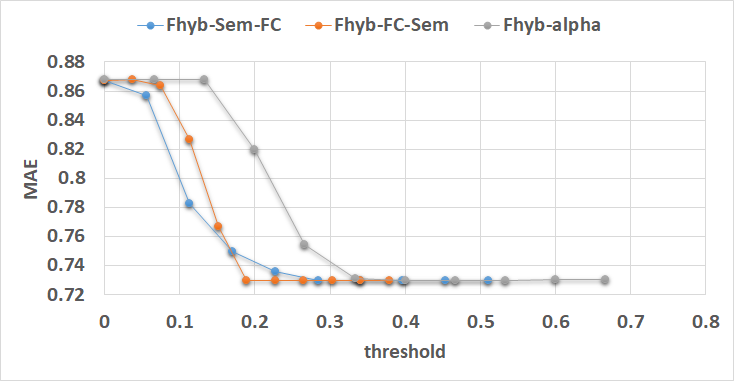
\includegraphics[width=0.9\textwidth]{hybsansclass.PNG}
	\caption{Évaluation MAE de l'hybridation sans classification des algorithmes FC et FSem}
	\label{fig:hybsansclassMAE}
\end{figure}

\begin{figure}[H]
	\centering
	\includegraphics[width=0.9\textwidth]{hybsansclassRMSE.PNG}
	\caption{Évaluation RMSE de l'hybridation sans classification des algorithmes FC et FSem}
	\label{fig:hybsansclassRMSE}
\end{figure}

Le tableau suivant présente les meilleures valeurs d'Alpha :
\begin{table}[H]
	\centering
	\begin{tabular}{|l|l|}
		\hline
		threshold & Best Alpha for threshold \\ \hline
		0 & 1 \\ \hline
		0.066666667 & 1 \\ \hline
		0.133333333 & 1 \\ \hline
		0.2 & 8 \\ \hline
		0.266666667 & 8 \\ \hline
		0.333333333 & 8 \\ \hline
		0.4 & 7 \\ \hline
		0.466666667 & 5 \\ \hline
		0.533333333 & 5 \\ \hline
		0.6 & 5 \\ \hline
		0.666666667 & 5 \\ \hline
	\end{tabular}
\captionof{table}{Tableau des differents seuils combiné à Alpha du FHyb pondéré}
\end{table}

Le tableau suivant \ref{tab:hyb} décrit les trois meilleures valeurs obtenues pour chaque algorithme en termes de MAE et RMSE.
\begin{table}[H]
	\centering
	\begin{tabular}{|l|l|l|l|}
		\hline
		threshold & 0.189 & 0.151 & 0.113 \\ \hline
		MAE  (FHyb-FC-Sem) & 0.73 & 0.767 & 0.827 \\ \hline
		RMSE (FHyb-FC-Sem) & 1.003 & 1.046 & \textbf{1.101} \\ \hline\hline
		threshold & 0.284& 0.227 & 0.17 \\ \hline
		MAE  (FHyb-Sem-FC) & 0.73 & 0.736 & 0.75 \\ \hline
		RMSE (FHyb-Sem-FC) & \textbf{1.001} & 1.007 & 1.023 \\ \hline\hline
		threshold & 0.466 & 0.533 & 0.6 \\ \hline
		Alpha & 0.5 & 0.5 & 0.5 \\ \hline
		MAE  (FHyb-alpha) & \textbf{0.7295} & 0.73 & 0.7301 \\ \hline
		RMSE (FHyb-alpha) & 1.0014 & 1.0018 & 1.002 \\ \hline
	\end{tabular}
	\captionof{table}{Récapitulatif des trois meilleurs résultats (MAE et RMSE) pour le FHyb pondéré}
	\label{tab:hyb}
\end{table}


\subsubsection*{Discussion des résultats}
Nous pouvons déduire de ces résultats que les trois hybridations donnent des résultats approximativement proches avec comme meilleure valeur de MAE égale à 0.73 et RMSE égale à 1.
Cependant, le FHyb pondéré à donnée la meilleurs valeurs de MAE qui est égale à 0.729 avec la valeur Alpha égales à 5.

\subsubsection*{FHyb avec classification}
Pour cette approche, nous ferons varier la valeur du nombre de clusters K dans les algorithmes suivants:
\begin{itemize}
\item FHyb pondéré K-NN (FHyb-alpha).
\item FHyb pondéré K-medoids (FHyb-alpha-Kmedoids).
\item FHyb collaboratif basé sémantique K-NN (FHyb-FC-Sem-KNN).
\item FHyb collaboratif basé sémantique K-medoids (FHyb-FC-Sem-Kmedoids).
\item FHyb collaboratif basé sémantique K-medoids et BSO (FHyb-FC-Sem-Kmedoids-BSO).
\item FHyb sémantique basé collaboratif K-NN (FHyb-Sem-FC-KNN).
\item FHyb sémantique basé collaboratif K-medoids (FHyb-Sem-FC-Kmedoids).
\item FHyb sémantique basé collaboratif K-medoids et BSO (FHyb-Sem-FC-Kmedoids-BSO).
\item FHyb Multivues K-NN (FHyb-Multiview-KNN).
\end{itemize}
\begin{figure}[H]
	\centering
	\includegraphics[width=0.9\textwidth]{hybclassMAE.PNG}
	\caption{Évaluation MAE des algorithmes hybrides basés classification}
	\label{fig:hybclassMAE}
\end{figure}


\begin{figure}[H]
	\centering
	\includegraphics[width=0.9\textwidth]{hybclassRMSE.PNG}
	\caption{Évaluation RMSE des algorithmes hybrides basés classification}
	\label{fig:hybclassRMSE}
\end{figure}

Le tableau suivant décrit les trois meilleures valeurs obtenues pour chaque algorithme en termes de MAE et RMSE.
\begin{table}[H]
	\centering
	\begin{tabular}{|l|l|l|l|}
		\hline
		k & 27 & 25 & 30 \\ \hline
		MAE(FHyb-FC-Sem-KNN) & \textbf{0.7171} &  0.7181 & 0.7185 \\ \hline
		RMSE(FHyb-FC-Sem-KNN)& \textbf{0.9946} &  0.9967 & 0.9950 \\ \hline\hline
		k & 15 & 45 & 30 \\ \hline
		MAE(FHyb-Sem-FC-KNN) & 0.7256& 0.7261& 0.7272 \\ \hline
		RMSE(FHyb-Sem-FC-KNN) & 1.003 & 1.0015 & 1.0030 \\ \hline\hline
		k & 65 & 55 & 45 \\ \hline
		MAE(FHyb-FC-Sem-Kmedoids-BSO) & 0.73001 & 0.7302 & 0.73064 \\ \hline
		RMSE(FHyb-FC-Sem-Kmedoids-BSO) & 1.0029 & 1.0029 & 1.0013 \\ \hline\hline
		k & 10 & 15 & 20 \\ \hline
		MAE(FHyb-Sem-FC-Kmedoids-BSO) & 0.7289 & 0.7309 & 0.7302 \\ \hline
		RMSE(FHyb-Sem-FC-Kmedoids-BSO) & 1.001 & 1.0034 & 1.0025 \\ \hline\hline
		k & 65 & 55 & 45 \\ \hline
		MAE(multiview\_knn\_svd) & 0.7300 & 0.7302 & 0.7306\\ \hline
		RMSE(multiview\_knn\_svd) & 1.0009 & 1.0017 & 1.0015 \\ \hline\hline
		k & 15 & 80 & 20 \\ \hline
		MAE(FHyb-Multiview-KNN) & 0.7294 & 0.7298 & 0.730\\ \hline
		RMSE(FHyb-Multiview-KNN) & 0.9994& 1.0015 & 0.9990 \\ \hline\hline
		k & 25 & 15 & 20 \\ \hline
		MAE(FHyb-Sem-FC-Kmedoids) & 0.7323 & 0.7324& 0.733 \\ \hline
		RMSE(FHyb-Sem-FC-Kmedoids) & 1.005& 1.004 & 1.0065 \\ \hline\hline
		k & 140 & 120 & 135 \\ \hline
		alpha & 0.1 & 0.4 & 0.6 \\ \hline
		MAE(FHyb-alpha-KNN) & 0.7287 & 0.7289 & 0.7289 \\ \hline
		RMSE(FHyb-alpha-KNN)& 0.9991 & 0.9991 & 0.9994\\ \hline\hline
		k & 15 & 20 & 10 \\ \hline
		alpha & 0.1 & 0.2 & 0.3 \\ \hline
		MAE(FHyb-alpha-Kmedoids) & 0.7300& 0.731 & 0.7312 \\ \hline
		RMSE(FHyb-alpha-Kmedoids) & 1.0015 & 1.0039 & 1.0021 \\ \hline
	\end{tabular}
\captionof{table}{Récapitulatif des trois meilleurs résultats (MAE et RMSE) pour les differents FHyb avec classification}
\end{table}
\subsubsection*{Discussion des résultats}
\myparagraph{FHyb pondéré} Pour ce filtrage l'ajout du clustering n'a pas amélioré les performances de la prédiction, car le Fhyb pondéré donne comme meilleure résultat 0.729 pour MAE et 1.001 pour RMSE, après l'ajout du clustering, MAE est passée à 0.730 et RMSE est restée presque la même.
Cependant l'ajout de la classification K-NN, a amélioré les performances de MAE qui est devenu 0.7287 et de RMSE qui est passé à 0.99.
 
\myparagraph{FHyb sémantique basé collaboratif} Après avoir incorporer le clustering K-medoids à ce filtrage, nous constatons que les évaluations ne se sont pas améliorées, car sans clustering MAE été égale à 0.73 et RMSE à 1.00, après l'ajout du clustering MAE est passée à 0.732 et RMSE est restée la même, donc on suppose que le choix des medoids d'une façon optimisée peut montrer l'apport du clustering, après avoir ajouté l'optimisation BSO, RMSE n'a pas changé mais MAE s'est améliorée et est passée à 0.728, donc le clustering optimisé est efficace sur ce filtrage.
Après l'ajout de la classification avec K-NN à ce filtrage, nous remarquons que MAE s'est améliorée et est devenu égale à 0.725, pour RMSE pas de changement à noter, donc la classification pour ce filtrage améliore la qualité de MAE seulement.

\myparagraph{FHyb collaboratif basé sémantique}
Ce filtrage sans classification a donnée comme meilleur résultat pour MAE=0.73 et RMSE=1.00, après l'ajout du clustering, MAE c'est améliorée et est passé à 0.729 et RMSE à 0.999 mais l'ajout de l'optimisation ne semble pas améliorer les performances de ces deux évaluations car elles ont passée respectivement à 0.73 et 1.00. Cependant l'ajout de la classification semble être la meilleure option à choisir pour ce filtrage car elle a fait passé MAE à 0.717 et RMSE à 0.994, donc elle est plus efficace que le clustering et le clustering optimisé.

\myparagraph{FHyb Multivues K-NN}
Ce filtrage utilise que la classification K-NN pour hybrider les deux vue sémantique et collaboratif, nous pouvons constaté qu'il a donné une valeur de 0.73 pour MAE et une valeur de 1.00 pour RMSE, donc pour cette base de donnée cette approche ne semble pas meilleure que les filtrages hybrides standard proposé ou avec classification car nous avons eu des performances mieux que celle-ci. 
Nous supposons que cette approche serait meilleure testée sur un autre dataset, de ce fait par la suite nous allons testé cette approche sur un autre jeu de données.

\subsubsection*{Comparaison des résultats avec d'autre méthodes utilisée sur MovieLens}
Pour voir si nos résultats sont de bonne qualité, nous avons décidé de les comparés à des méthodes déjà utilisé sur le dataset MovieLens 100k, les résultats peuvent être consultés sur le site \cite{ref42}.
Le tableau suivant est un récapitulatif de nos meilleurs résultats pour chaque approches développées:

\begin{table}[H]
	\centering
	\begin{tabular}{|l|l|l|}
		\hline
		& MAE & RMSE \\ \hline
		FC standard & 0.73 & 1.001 \\ \hline
		FC basé k-medoids & 0.733 & 1.004 \\ \hline
		FC basé k-medoids et BSO & 0.728 & 1.001 \\ \hline
		FC basé K-NN & 0.73 & 1.001 \\ \hline
		FSem standard & 0.729 & 1.002 \\ \hline
		FSem k-medoids & 0.730 & 1.001 \\ \hline
		FSem k-medoids et BSO & 0.728 & 1.002 \\ \hline
		FSem K-NN & 0.729 & 1.000 \\ \hline
		FHyb pondéré & 0.729 & 1.001 \\ \hline
		FHyb pondéré k-medoids & 0.730 & 1.001 \\ \hline
		FHyb pondéré K-NN & 0.728 & 0.991 \\ \hline
		FHyb Sem basé FC & 0.73 & 1.001 \\ \hline
		FHyb Sem basé FC k-medoids & 0.732 & 1.005 \\ \hline
		FHyb Sem basé FC k-medoids et BSO & 0.728 & 1.001 \\ \hline
		FHyb Sem basé FC K-NN & 0.725 & 1.003 \\ \hline
		FHyb FC basé Sem & 0.730 & 1.003 \\ \hline
		FHyb FC basé Sem k-medoids & 0.729 & 0.999 \\ \hline
		FHyb FC basé Sem k-medoids et BSO & 0.730 & 1.002 \\ \hline
		FHyb FC basé Sem K-NN & \cellcolor[HTML]{67FD9A}0.717 & \cellcolor[HTML]{67FD9A}0.994 \\ \hline
		FHyb mutivues K-NN & 0.730 & 1.000 \\ \hline
	\end{tabular}
\captionof{table}{Récapitulatif des meilleurs résultats (MAE et RMSE) pour touts les filtrages conçus}
 \label{tab:movie}
\end{table}
Le tableau suivant montre les résultats obtenu à partir du site \cite{ref42}.
Les deux méthodes utilisés sont SVDplusplus qui est une amélioration de la méthode SVD et UserKNNPearson qui est un filtrage collaboratif avec la corrélation de Pearson comme distance entre utilisateur et une classification des voisins des ces derniers avec l'algorithme K-NN.
\begin{table}[H]
	\centering
	\begin{tabular}{|l|l|l|}
		\hline
		& MAE & RMSE \\ \hline
		UserKNNPearson & 0.728 & 0.929 \\ \hline
		SVDPlusPlus version 1& 0.718 & 0.913 \\ \hline
		SVDPlusPlus  version 2& \cellcolor[HTML]{67FD9A} 0.713 & \cellcolor[HTML]{67FD9A}0.90829	\\ \hline
	\end{tabular}
\captionof{table}{Les meilleurs résultats (MAE et RMSE) trouvrer à partir de \cite{ref42} pour le dataset MovieLens 100k}
 \label{tab:mymedia}
\end{table}
Nous pouvons conclure que nos résultats sont dans les normes comparé avec ceux déjà développé ou part avant, de plus nous nous rapprochons avec notre méthode FHyb FC basé Sem et K-NN du résultat de SVDPlusPlus version 2 du tableau .
Sachant que la méthode de SVDPlusPlus prend beaucoup de temps pour s'exécutée, il serait possible d'opter pour notre approche qui est FHyb FC basé Sem et K-NN, qui s'exécutera plus rapidement que SVDPlusPlus, de plus notre approche est simple à implémenter et donne des résultats proches de la méthode SVDPlusPlus.\\


%%%%%%%%%%%%%%%%%%%%%%%%%%%%%%%%%%%%%%%%%%%%%%%%%%%%%%%%%%%%%
\textbf{B) Evaluations avec RED}\\
Afin de confirmer les résultats obtenus de nos approches sur le dataset MovieLens, nous avons décidé de refaire les testes sur un autre dataset qui est RED.
Nous avons choisi de refaire les testes que sur les approches qui ont donné de bons résultats, car nous somme limé par le temps et la puissance de calcul de nos machines.
\subsubsection*{Évaluations}
Dans cette partie, nous réaliserons un ensemble de tests portant sur les performances de notre approche et nous comparerons nos résultats avec les résultats des approches existantes. \\

\begin{enumerate}[nosep,label=\textbf{\arabic*)}]
	%%  \setcounter{enumi}{4}
	\item \textbf{Filtrage collaboratif avec classification et classification optimisée}
\end{enumerate}\mbox{}\indent{} Dans cette phase d’expérimentations, nous allons évaluer la qualité de la recommandation lorsque celle-ci est basée sur un FC basé K-medoids, FC basé K-medoids et BSO et FC basé K-NN. Nous ferons des expérimentations par rapport à la corrélation de Pearson, étant donné que celle-ci reste l’une des plus connues et des plus utilisées, et comme prétraitement du dataset nous avons opté pour la méthode SVD vu son efficacité d'après les testes précédent.
\begin{figure}[H]
	\centering
	\includegraphics[width=\textwidth]{epFCMAE.PNG}
	\caption{Évaluation MAE du FC avec classification sur RED}
	\label{fig:epFCMAE}
\end{figure}

\begin{figure}[H]
	\centering
	\includegraphics[width=\textwidth]{epFCRMSE.PNG}
	\caption{Évaluation RMSE du FC avec classification sur RED}
	\label{fig:epFCRMSE}
\end{figure}
Le tableau suivant décrit les trois meilleures valeurs obtenues en termes de MAE et RMSE.
\begin{table}[H]
	\centering
	\begin{tabular}{|l|l|l|l|}
		\hline
		k & 5 & 17 & 11 \\ \hline
		MAE(FC-user-user-KNN) & 0.7744 & 0.779 & 0.7798 \\ \hline
		RMSE(FC-user-user-KNN) & 1.066& 1.0709 & 1.0712 \\ \hline\hline
		k & 17 & 36 & 64 \\ \hline
		MAE(FC-user-user-Kmedoids-BSO) & \textbf{0.7677} & 0.7697  & 0.7684 \\ \hline
		RMSE(FC-user-user-Kmedoids-BSO) &\textbf{1.060} & 1.0697  & 1.07534 \\ \hline\hline
		k & 19 & 23 & 48 \\ \hline
		MAE(FC-user-user-Kmedoids) & 0.7751& 0.7753 & 0.7785\\ \hline
		RMSE(FC-user-user-Kmedoids) & 1.0659 & 1.06989 & 1.0814 \\ \hline
	\end{tabular}
\captionof{table}{Récapitulatif des trois meilleurs résultats (MAE et RMSE) pour le FC avec classification du dataset RED}
\end{table}
\subsubsection*{Discussion des résultats}
D'après le tableau récapitulatif et les graphes ci-dessus, nous constatons que l'approche qui donne les meilleurs résultats est le FC basé K-medoids et BSO avec MAE égale à 0.767 et RMSE égale à 1.060, ce qui confirme l'apport de l'optimisation sur le clustering.\\


%%%%%%%%%%%%%%%%%%%EP SEM%%%%%%%%%%%%%%%%%%%%%%%%%%%%%%
\begin{enumerate}[nosep,label=\textbf{\arabic*)}]
	\setcounter{enumi}{1}
	\item \textbf{Filtrage sémantique  avec classification et classification optimisée}
\end{enumerate}\mbox{} \indent Dans cette partie, nous allons évalué la qualité de la recommandation lorsque celle-ci est basée sur un FSem basé K-medoids, FSem basé K-medoids et BSO et FSem basé K-NN.  Nous ferons des expérimentations en utilisant la formule de distance d'intérêt entre utilisateur, et la distance de Wu and Palmer entre les items car le dataset RED possède une représentation sous forme d'ontologie des items.
Le prétraitement des valeurs manquantes est effectué avec la méthode SVD.
\begin{figure}[H]
	\centering
	\includegraphics[width=\textwidth]{epsemMAE.PNG}
	\caption{Évaluation MAE du FSem avec classification sur RED}
	\label{fig:epsemMAE}
\end{figure}

\begin{figure}[H]
	\centering
	\includegraphics[width=\textwidth]{epsemRMSE.PNG}
	\caption{Évaluation RMSE du FSem avec classification sur RED}
	\label{fig:epsemRMSE}
\end{figure}
La tableau suivant décrit les trois meilleures valeurs en termes de MAE et RMSE.
\begin{table}[H]
	\centering
	\begin{tabular}{|l|l|l|l|}
		\hline
		k & 12 & 32 & 46 \\ \hline
		MAE(FSem-user-user-Kmedoids) & 0.7765& 0.7771 & 0.7779\\ \hline
		RMSE(FSem-user-user-Kmedoids) & 1.0753 & 1.0775 & 1.0823 \\ \hline\hline
		k & 8 & 7 & 6 \\ \hline
		MAE(FSem-user-user-KNN) & 0.7778 & 0.7812 & 0.7832 \\ \hline
		RMSE(FSem-user-user-KNN) & 1.0790 & 1.0806 & 1.0834 \\ \hline\hline
		k & 43 & 20 & 46 \\ \hline
		MAE(FSem-user-user-Kmedoids-BSO) & \textbf{0.7637} & 0.7664 & 0.7664 \\ \hline
		RMSE(FSem-user-user-Kmedoids-BSO) & \textbf{1.064} & 1.0681 & 1.0750 \\ \hline
	\end{tabular}
\captionof{table}{Récapitulatif des trois meilleurs résultats (MAE et RMSE) pour le FSem avec classification du dataset RED}
\end{table}
\subsubsection*{Discussion des résultats}
D'après le tableau récapitulatif et les graphes ci-dessus, nous constatons que l'approche qui donne les meilleurs résultats est le FSem basé K-medoids et BSO avec MAE égale à 0.763 et RMSE égale à 1.064, ce qui confirme l'apport de l'optimisation sur le clustering.\\


%%%%%%%%%%%%%%%%%EP HYB%%%%%%%%%%%%%%%%%%%%%%%%%%%%%%%%%%%
\begin{enumerate}[nosep,label=\textbf{\arabic*)}]
	  \setcounter{enumi}{2}
	\item \textbf{Filtrage hybride avec classification et classification optimisée}
\end{enumerate}\mbox{}\indent Dans cette partie, nous allons évalué la qualité de la recommandation lorsque celle-ci est basée sur un FHyb basé K-medoids, FHyb basé K-medoids et BSO et FHyb basé K-NN.  Nous ferons des expérimentations par rapport à la corrélation de Pearson, étant donné que celle-ci reste l’une des plus connues et des plus utilisées, et comme prétraitement du dataset nous avons opté pour la méthode SVD vu son efficacité d'après les testes précédent.

\begin{figure}[H]
	\centering
	\includegraphics[width=\textwidth]{ephybMAE.PNG}
	\caption{Évaluation MAE du filtrage hybride avec classification sur RED}
	\label{fig:ephybMAE}
\end{figure}


\begin{figure}[H]
	\centering
	\includegraphics[width=\textwidth]{ephybRMSE.PNG}
	\caption{Évaluation RMSE du filtrage hybride avec classification sur RED}
	\label{fig:ephybRMSE}
\end{figure}
Le tableau suivant décrit les trois meilleurs valeurs obtenues pour chaque algorithme en termes de MAE et RMSE.
\begin{table}[H]
	\centering
	\begin{tabular}{|l|l|l|l|}
		\hline
		k & 10 & 8 & 11 \\ \hline
		MAE(FHyb-FC-Sem-KNN) & 0.7791 & 0.7812 & 0.7818 \\ \hline
		RMSE(FHyb-FC-Sem-KNN) & 1.0728 & 1.07503 & 1.07846 \\ \hline\hline
		k & 9 & 7 & 8 \\ \hline
		MAE(FHyb-Multiview) & \textbf{0.7657}& 0.7744 & 0.7744 \\ \hline
		RMSE(FHyb-Multiview) & \textbf{1.0703}& 1.0781 & 1.0812\\ \hline\hline
		k & 34 & 10 & 6 \\ \hline
		MAE(FHyb-FC-Sem-Kmedoids) & 0.784 & 0.7852 & 0.7865 \\ \hline
		RMSE(FHyb-FC-Sem-Kmedoids) & 1.0850 & 1.0762 & 1.07503 \\ \hline\hline
		k & 38 & 13 & 17 \\ \hline
		MAE(FHyb-FC-Sem-Kmedoids-BSO) & 0.7798 & 0.78053 & 0.7812 \\ \hline
		RMSE(FHyb-FC-Sem-Kmedoids-BSO) & 1.0825 & 1.0765 & 1.0769 \\ \hline
	\end{tabular}
\captionof{table}{Récapitulatif des trois meilleurs résultats (MAE et RMSE) pour le FHyb avec classification du dataset RED}
\end{table}

\subsubsection*{Discussion des résultats}
D'après le tableau récapitulatif et les graphes ci-dessus, nous constatons que l'approche qui donne les meilleurs résultats dans le cas d'un filtrage hybride est le FHyb multivues K-NN avec MAE égale à 0.765 et RMSE égale à 1.070, c'est l'approche inspiré du travail de \cite{ref30}.

\subsubsection*{Comparaison des résultats avec d'autre méthodes utilisée sur RED}
Pour voir si nos résultats sont de bonne qualité et dans les normes, nous avons décidé de les comparés à des méthodes déjà utilisé sur le dataset RED, les résultats peuvent être consultés sur le site \cite{ref43}.
Le tableau suivant est un récapitulatif de nos meilleurs résultats pour chaque approches développées:

\begin{table}[H]
	\centering
	\begin{tabular}{|l|l|l|}
		\hline
		             & MAE & RMSE \\ \hline
		FC basé K-NN & 0.774 & 1.065 \\ \hline
		FC basé k-medoids & 0.775 & 1.065 \\ \hline
		FC basé k-medoids et BSO & 0.767 & 1.060 \\ \hline
		FSem basé K-NN & 0.778 & 1.079 \\ \hline
		FSem basé k-medoids & 0.776 & 1.075 \\ \hline
		FSem basé k-medoids et BSO & \cellcolor[HTML]{67FD9A}0.763 & \cellcolor[HTML]{67FD9A}1.064 \\ \hline
		FHyb collaboratif basé sémantique K-NN & 0.779 & 1.072 \\ \hline
		FHyb collaboratif basé sémantique  et k-medoids & 0.784 & 1.085 \\ \hline
		FHyb collaboratif basé sémantique et k-medoids-BSO & 0.779 & 1.082 \\ \hline
		FHyb multivues & 0.765 & 1.070 \\ \hline
	\end{tabular}
\captionof{table}{Récapitulatif des meilleurs résultats (MAE et RMSE) pour les differents filtrage conçu et testés sur RED}
\end{table}
Sur le site \cite{ref43}, le meilleur résultat de MAE est de 0.804, et 1.047 pour RMSE avec la méthode SVD. En comparant nos résultats avec celui du site, nous pouvons dire que nous avons amélioré nettement MAE avec notre approche qui est FSem basé K-medoids et BSO avec MAE égale à 0.763, pour RMSE il n'y a pas une grande différence entre notre approche et SVD. Par conséquent nous avons prouvé l'efficacité de notre méthode comparé aux méthodes déjà appliqué sur le dataset RED.

\section{Récapitulatif des différents résultats des évaluations}
Dans cette partie nous allons récapituler les différents résultats obtenus pour chaque filtrage réalisé, en termes  d'hybridation, de classification et de classification optimisée sur les deux dataset utilisés.
\begin{enumerate}[nosep,label=\textbf{\arabic*)}]
	%%\setcounter{enumi}{2}
	\item Filtrage collaboratif
\end{enumerate}\mbox{} \indent
Pour le filtrage collaboratif standard, le clustering optimisé avec l'algorithme K-medoids et BSO a amélioré les résultats du FC standard.
En utilisant la classification avec K-NN sur le FC standard, cela n'a pas apporté d'amélioration. Donc pour le FC le meilleur filtrage est le FC basé K-medoids et BSO, il a pu donner des résultats très proches à ceux des algorithmes déjà appliqués sur MovieLens, d'environ 0.015 de différence pour MAE et de 0.092 pour RMSE.\\

\begin{enumerate}[nosep,label=\textbf{\arabic*)}]
	\setcounter{enumi}{1}
	\item \ Filtrage sémantique
\end{enumerate}\mbox{} \indent
Le FSem standard n'a pas pu être amélioré ni par la classification avec K-NN et ni par le clustering optimisé. Mais ses résultats restent dans les normes comparé aux résultats données par d'autres méthodes appliquées sur le dataset MovieLens, avec MAE égale à 0.7297 et RMSE égale à 1.0012.
En appliquant le FSem basé K-medoids, le FSem basé K-medoids-BSO et le FSem basé K-NN sur le dataset RED, nous avons obtenus de très bons résultats comparé à ceux du site \cite{ref43}.\\

\begin{enumerate}[nosep,label=\textbf{\arabic*)}]
	\setcounter{enumi}{2}
	\item Filtrage hybride
\end{enumerate}\mbox{} \indent
L'approche que nous avons conçue et qui a donné les meilleures performances sur le dataset MovieLens est le FHyb collaboratif basé sémantique et K-NN, ce résultat et très proche des meilleurs performance existantes de ce dataset (voir les deux tableaux \ref{tab:mymedia} et \ref{tab:movie}).

\subsubsection*{Comparaison entre les résultats de MovieLens et RED}
En rajoutant la classification et classification optimisée aux trois types de filtrages et après les avoirs testés sur le dataset RED, nous avons obtenu de très bons résultat comparé a ceux du site \cite{ref43}, et nous pouvons ainsi conclure et dire qu'il y'a un apport lors de l'ajout de la classification et la classification optimisée aux  différent types de filtrage conçus, car cela nous a permis de nous rapprocher des meilleurs résultats déjà existants dans le cas du dataset MovieLens, et de surpasser les performances des algorithmes déjà existants en utilisant le dataset RED.
\section{Conclusion}
Dans ce chapitre que nous clôturons, nous avons pu tester différents algorithmes
de recommandation que nous avons réalisé sur les datasets MovieLens 100k et RED.
En effet, ces expérimentations nous ont permis de faire des comparaison entre les différents filtrages conçus, et de conclure en disant que les filtrages conçus se sont montrés très efficace sur le dataset RED. Nous avons pu nous rapprocher des résultats déjà existants sur le dataset MovieLens avec notre approche (FHyb collaboratif basé sémantique et K-NN) qui est simple et plus rapide que SVDPlusPlus.  

\newpage
\input{annex}


\newpage
\newpage
\addcontentsline{toc}{chapter}{Bibliographie} 

\begin{thebibliography}{100}
	%%auteur1, auteur2, auteur3 (sinon auteur1 and all ida kano plus de 3). Le titre complet. Page. Année
\pagenumbering{Roman}
\bibitem{ref1} Haydar, Charif Alchiekh. Les systèmes de recommandation à base de confiance. Diss. Université de Lorraine, 2014.


\bibitem{ref2}Benouaret, Idir. Un système de recommandation contextuel et composite pour la visite personnalisée de sites culturels. Diss. Université de Technologie de Compiègne, 2017.

\bibitem{ref3} CHARU, C. AGGARWAL. Recommender Systems: The Textbook. Springer, 2018.

\bibitem{ref4}  Balabanović, Marko, and Yoav Shoham. "Fab: content-based, collaborative recommendation." Communications of the ACM 40.3 (1997): 66-72.

\bibitem{ref5} Rao, K. Nageswara. "Application domain and functional classification of recommender systems—a survey." DESIDOC Journal of Library \& Information Technology 28.3 (2008): 17-35.

\bibitem{ref6} Les systèmes de recommandation : une catégorisation. [en ligne], \url{https://interstices.info/les-systemes-de-recommandation-categorisation/} Page consultée le 11/06/2019.

\bibitem{ref7} Recommender systems-How they works and their impacts. [en ligne], \url{http://findoutyourfavorite.blogspot.com/2012/04/content-based-filtering.html} Page consultée le 11/06/2019.


\bibitem{ref8} Sulieman, Dalia. Towards semantic-social recommender systems. Diss. Cergy-Pontoise, 2014.

\bibitem{ref9} Esslimani, Ilham, Armelle Brun, and Anne Boyer. "Behavioral similarities for collaborative recommendations," 2008.

\bibitem{ref10} Berrut, Catherine, and Nathalie Denos. "Filtrage collaboratif." 2003.

\bibitem{ref11} Belloui, Amokrane. "Lusage Des Concepts Du Web Smantique Dans Le Filtrage Dinformation Collaboratif." Institut National dInformatique Alger, 2008.

\bibitem{ref12} Burke, Robin. "Hybrid recommender systems: Survey and experiments." User modeling and user-adapted interaction 12.4 (2002): 331-370.

\bibitem{ref13} Gruber, Thomas R. "A translation approach to portable ontology specifications." Knowledge acquisition 5.2 (1993): 199-220.

\bibitem{ref14} Petrakis, Euripides GM, et al. "X-similarity: Computing semantic similarity between concepts from different ontologies." Journal of Digital Information Management 4.4, 2006.

\bibitem{ref15}  Rada, Roy, et al. "Development and application of a metric on semantic nets." IEEE transactions on systems, man, and cybernetics 19.1 (1989): 17-30. 

\bibitem{ref16} Resnik, Philip. "Using information content to evaluate semantic similarity in a taxonomy." arXiv preprint cmp-lg/9511007, 1995.

\bibitem{ref17} Seco, Nuno, Tony Veale, and Jer Hayes. "An intrinsic information content metric for semantic similarity in WordNet." Ecai. Vol. 16. 2004.

\bibitem{ref18}Lin, Dekang. "An information-theoretic definition of similarity." Icml. Vol. 98. No. 1998. 1998.

\bibitem{ref19} Jiang, Jay J., and David W. Conrath. "Semantic similarity based on corpus statistics and lexical taxonomy." arXiv preprint cmp-lg/9709008, 1997.

\bibitem{ref20} Bouzeghoub, Mokrane, and Dimitre Kostadinov. "Personnalisation de l'information: aperçu de l'état de l'art et définition d'un modèle flexible de profils." CORIA 5, 2005 : 201-218.


\bibitem{ref21} Brusilovsky, Peter. "Adaptive educational hypermedia." International PEG Conference. Vol. 10. 2001.

\bibitem{ref22} 
Les algorithmes de recommandation
By Mathieu [en ligne], \url{https://www.podcastscience.fm/dossiers/2012/04/25/les-algorithmes-de-recommandation/}, Page consultée le 11/06/2019


\bibitem{ref23} Bouneffouf, Djallel. DRARS, a dynamic risk-aware recommender system. Diss. 2013.


\bibitem{ref24} Salton, Gerard, Anita Wong, and Chung-Shu Yang. "A vector space model for automatic indexing." Communications of the ACM 18.11, 1975 : 613-620.


\bibitem{ref25} Picot-Clémente, Romain, Cécile Bothorel, and Philippe Lenca. "Towards Intention, Contextual and Social Based Recommender System." Advanced Approaches to Intelligent Information and Database Systems. Springer, Cham, 2014. 3-13.

\bibitem{ref26} Daoud, Mariam, et al. "Construction des profils utilisateurs à base d'une ontologie pour une recherche d'information personnalisée." francophone en Recherche d'Information et Applications (CORIA 2008). 2008.


\bibitem{ref27} Zemirli, Nesrine, and Shrooq Alsenan. "PERSO-Retailer: Toward a Web Content Management System Based on a Personalized Marketing Recommender System for Retailers." 2015 International Conference on Cloud Computing (ICCC). IEEE, 2015.


\bibitem{ref28} Sieg, Ahu, Bamshad Mobasher, and Robin Burke. "Web search personalization with ontological user profiles." Proceedings of the sixteenth ACM conference on Conference on information and knowledge management. ACM, 2007.

\bibitem{ref29} 
Difference between Taxonomy and Ontology [en ligne], \url{http://www.differencebetween.info/difference-between-taxonomy-and-ontology}, Page consultée le 11/06/2019


\bibitem{ref30} Guo, Guibing, Jie Zhang, and Neil Yorke-Smith. "Leveraging multiviews of trust and similarity to enhance clustering-based recommender systems." Knowledge-Based Systems 74, 2015 : 14-27.

\bibitem{ref31} 
Introduction to Recommender System. Part 1 (Collaborative Filtering, Singular Value Decomposition) [en ligne], \url{https://hackernoon.com/introduction-to-recommender-system-part-1}, Page consultée le 11/06/2019.

\bibitem{ref31} Ujjin, Supiya, and Peter J. Bentley. "Particle swarm optimization recommender system." Proceedings of the 2003 IEEE Swarm Intelligence Symposium. SIS'03 (Cat. No. 03EX706). IEEE, 2003.

\bibitem{ref32} 
Introduction à l’algorithme K Nearst Neighbors (K-NN) [en ligne], \url{https://mrmint.fr/introduction-k-nearest-neighbors},  Page consultée le 11/06/2019.

\bibitem{ref33} Han, Jiawei, Jian Pei, and Micheline Kamber. Data mining: concepts and techniques. Elsevier, 2011.


\bibitem{ref34}
Drias, Habiba, Souhila Sadeg, and Safa Yahi. "Cooperative bees swarm for solving the maximum weighted satisfiability problem." International Work-Conference on Artificial Neural Networks. Springer, Berlin, Heidelberg, 2005.

\bibitem{ref35} Bellahmer Meziane. Recommandation par filtrage collaboratif basé sur un clustering optimisé, mémoire de fin d'étude. 2018.


\bibitem{ref36} Shambour, Qusai, and Jie Lu. "A hybrid multi-criteria semantic-enhanced collaborative filtering approach for personalized recommendations." Proceedings of the 2011 IEEE/WIC/ACM International Conferences on Web Intelligence and Intelligent Agent Technology-Volume 01. IEEE Computer Society, 2011.

\bibitem{ref37} Wu, Zhibiao, and Martha Palmer. "Verbs semantics and lexical selection." Proceedings of the 32nd annual meeting on Association for Computational Linguistics. Association for Computational Linguistics, 1994.

\bibitem{ref38} Shet, K. C., and U. Dinesh Acharya. "A new similarity measure for taxonomy based on edge counting." arXiv preprint arXiv:1211.4709, 2012.

\bibitem{ref39} What is Python?[en ligne], \url{https://www.python.org/doc/essays/blurb/}, Page consultée le 11/06/2019.

\bibitem{ref40} What is Linux?[en ligne], \url{https://www.computerhope.com/jargon/l/linux.htm}, Page consultée le 11/06/2019.


\bibitem{ref41} Visual Studio Code[en ligne], \url{https://code.visualstudio.com/docs}, Page consultée le 11/06/2019.

\bibitem{ref42} MyMediaLite: Example Experiments[en ligne], \url{http://www.mymedialite.net/examples/datasets.html}, Page consultée le 11/06/2019.

\bibitem{ref43} LibRec Examples on Real Data Sets[en ligne], \url{https://librec.net/release/v1.3/example.html}, Page consultée le 11/06/2019.
\end{thebibliography}
\newpage
\thispagestyle{empty}
\begin{center}
	\textbf{\LARGE Résumé}
\end{center}

Le présent projet de fin d’études de master propose une approche de recommandation hybride, qui combine le Filtrage collaboratif (FC) et le filtrage sémantique (Fsem) selon différentes hybridations. Notre approche considère plusieurs méthodes du FC (basé utilisateur, AVG user, AVG Item, SVD) ; différentes mesures de similarité pour le FSem (Jacquard, Wu \& Palmer) ; et différentes hybridations (Filtrage pondéré, FC basé sémantique et FSem basé collaboratif). De plus, afin d’améliorer les performances de nos algorithmes nous avons utilisé des techniques de classification, supervisé (KNN) et non supervisé (Kmedoids) avec les différents algorithmes. Pour avoir le meilleur partitionnement, nous avons intégré l’algorithme d’optimisation BSO avec l’algorithmes de clustering BSO. Finalement, nous avons proposé une hybridation multi-vues basée sur KNN afin d’amélioré cette classification, en utilisant les deux vues collaborative et sémantique.
Les résultats des évaluations en utilisant deux bases différentes : la base MovieLens et la base RED ont montré que les algorithmes de filtrages basés sur la classification et la classification optimisée ont donné de bonnes performances sur la base RED, et ont donné des résultats très proches à ceux déjà existantes sur la base MovieLens.
\thispagestyle{empty}
\begin{center}
	\textbf{\LARGE 
		Abstract}
\end{center}
This master thesis project proposes a hybrid recommendation approach, which combines Collaborative Filtering (FC) and semantic filtering (Fsem) according to different hybridizations. Our approach considers several FC methods (user based, AVG user, AVG Item, SVD); different measures of similarity for the FSem (Jacquard, Wu \& Palmer); and different hybridizations (weighted filtering, semantic-based FC and collaborative-based FSem). Moreover, in order to improve the performances of our algorithms we used classification, supervised (KNN) and unsupervised (Kmedoids) techniques with the preciously mentioned algorithms. To have the best partitioning, we integrated the Bee Swam Optimiazation (BSO) algorithm with the different implemented clustering algorithms. Finally, we proposed a KNN-based multi-view hybridization to improve this classification, using both collaborative and semantic views.
The results of the evaluations using the two different databases: the MovieLens database and the RED database have shown that the classification and optimized classification filtering algorithms have given good performances on the RED database, and have given results very similar to those already existing on the database MovieLens.
\newpage


\end{document}